\documentclass[a4paper,11pt,hidelinks]{scrartcl}

% packages
\usepackage[ngerman]{babel}
\usepackage{graphicx}
\usepackage{subcaption}
\usepackage{url}
\usepackage{hyperref}
\usepackage{apacite}
\usepackage{tabularx}
\usepackage{makecell}
\usepackage{listings}
\usepackage{fontspec}
    \setmainfont{Vollkorn}
    \setsansfont{Lato}
    \setmonofont{Inconsolata}
\usepackage[htt]{hyphenat}
\usepackage{multicol}
\usepackage{amssymb}
\usepackage{amsmath}
\usepackage{tabto}
\usepackage[left=«,right=»]{dirtytalk}
\usepackage{float}
\usepackage{metalogo}

% global options
\renewcommand{\baselinestretch}{1.25}
\pagestyle{headings}

% macro definitions
\newcommand{\secref}[1]{{\ref{#1} \textit{\nameref{#1}}}, Seite \pageref{#1}}
\newcommand{\imgref}[1]{{Abbildung \ref{#1}, Seite \pageref{#1}}}
\newcommand{\tblref}[1]{{Tabelle \ref{#1}, Seite \pageref{#1}}}

% list of equations
\newfloat{equation}{H}{for}
\floatname{equation}{Formel}

% listings
\lstset{basicstyle=\ttfamily}

\begin{document}

\author{Patrick P. Bucher and  Christopher J. Christensen}
\title{OAuth 2}
\subtitle{Computer Science Hot Topics}
\date{\today}
\maketitle

\section*{Abstract}

OAuth 2 is a delegation protocol that lives within the context of HTTP. It is mainly used to connect websites to one another and to secure APIs exposed to the web. OAuth 2 enables resource owners to delegate (limited) access to clients without sharing their credentials. OAuth 2 is neither an authentication nor an authorization protocol, but it defines the mechanisms to build such protocols. It does not define any cryptographic mechanisms, but leaves those decisions open for the implementation. The authorization server plays a key role in every web application that is secured through the means of OAuth 2. This paper gives an overview of the components and mechanisms involved in an OAuth 2 secured web application. Furthermore, a demo OAuth 2 application is presented as a case study to elucidate the role of and communication between different components involved in an OAuth 2 deployment. The JWT token format and common vulnerabilities of OAuth 2 are the subject of additional chapters.

\newpage

\section*{Abstract}
\addcontentsline{toc}{section}{Abstract}

Die rheumatoide Arthritis ist eine Autoimmunerkrankung, bei der Gelenke angegriffen und irreversibel geschädigt werden. Die Erosion des Gelenkgewebes wird durch medizinisches Fachpersonal anhand von Röntgenbildern ermittelt, was pro Patient mehrere Minuten in Anspruch nimmt.

In einer Vorarbeit haben Janick Rohrbach (ZHAW), Tobias Reinhard (Seantis GmbH), Beate Sick (Universität Zürich) und Oliver Dürr (HTWG Konstanz) diesen Vorgang mithilfe von \textit{Deep Convolutional Neuronal Networks} automatisiert, wodurch eine gleichbleibende Bewertungsqualität gewährleistet wird. Das Ma\-chine-Learn\-ing-Modell wurde mit zehntausenden von klassifizierten Gelenken aus der SCQM-Datenbank (\textit{Swiss Clinical Quality Management in Rheumatic Disease}) trainiert, validiert und getestet.

Die vorliegende Arbeit beschreibt, wie auf Basis dieses und zweier weiterer Ma\-chine-Learn\-ing-Modelle (Erkennung von Körperteilen und Extraktion von Gelenken auf Röntgenbildern) ein Webservice erstellt wird, womit das automatische Scoring von Gelenken anderen Anwendungen zur Verfügung gestellt werden kann. Der resultierende Prototyp ist eine verteilte Anwendung, welche die bestehenden Ma\-chine-Learn\-ing-Modelle mithilfe von Messaging zu einem lose gekoppelten System zusammenfügt. Diese Architektur erlaubt es, mehrere Instanzen pro Modell auszuführen, wodurch die Röntgenbilder schnell und zuverlässig verarbeitet werden können.

Die Qualität des Gesamtsystems wird mit verschiedenen Metriken evaluiert. Damit können Qualitätsverbesserungen des Gesamtsystems beurteilt werden, wenn einzelne Ma\-chine-Learn\-ing-Komponenten durch neuere, verbesserte Versionen ersetzt werden. 

Im Ausblick wird behandelt, welche weiteren Schritte notwendig wären, um das System beim Auftraggeber in den Produktiveinsatz überführen zu können.

\newpage

\tableofcontents
\newpage

\section{Problemstellung}
\label{sec:Problemstellung}

Bei der rheumatoiden Arthritis handelt es sich um eine Autoimmunerkrankung, bei der sich das Gelenkgewebe entzündet. Halten diese Entzündungen über längere Zeit an, werden die betroffenen Gelenke dadurch irreversibel geschädigt.

Die Erosion des Gelenkgewebes wird durch Fachpersonal anhand von Röntgenbildern eingestuft. Hierzu wird die Ratingen-Score verwendet, die das Fortschreiten der Erosion auf einer Skala von 0\% (gesundes Gelenk) bis bis 100\% (Gelenkgewebe vollständig erodiert) abbildet. Diese Einschätzung wurde bisher manuell vorgenommen, was pro Röntgenbild mehrere Minuten dauert. Dieser Vorgang wird als \textit{Scoring} bezeichnet.

Im Rahmen einer Bachelorarbeit an der ZHAW \cite{rohrbach2017} und in einem Folgeprojekt im Rahmen einer Masterarbeit (nicht öffentlich verfügbar) haben sich Janick Rohrbach (Zürcher Hochschule für Angewandte Wissenschaften), Tobias Reinhard (Seantis GmbH), Beate Sick (Universität Zürich) und Oliver Dürr (HTWG Konstanz) mit der Automatisierung des Scorings befasst \cite{rohrbach2019}. Dadurch soll der Vorgang einerseits beschleunigt werden, andererseits soll auch eine gleichbleibende Bewertungsqualität gewährleistet werden. Diese Verbesserungen dürften sich gerade bei umfassenden und langfristigen Studien als hilfreich erweisen.

Die automatische Auswertung von Bildern mit klassischen Machine-Learning-Metho\-den gestaltete sich bisher als schwierig. Mithilfe von \textit{Deep Convolutional Neuronal Networks}, die geeignete Merkmale von Bildern selbständig herausarbeiten, konnten auf diesem Gebiet in den letzten Jahren grosse Fortschritte erzielt werden.

Auf Basis von Röntgenbildern aus der SCQM\footnote{\url{https://www.scqm.ch/ueber-uns/} (abgerufen am 10.05.2020)}-Datenbank konnte ein entsprechendes Modell mit zehntausenden klassifizierten Gelenken trainiert, validiert und getestet werden. Hierbei stellte die Unausgeglichenheit der Testdaten ‒ ca. zwei Drittel der Röntgenbilder zeigen gesunde Gelenke ‒ eine grosse Herausforderung dar. Dennoch konnte ein Ergebnis erzielt werden, das sich sehen lässt: So stimmen die Bewertungen des automatischen Modells besser mit denjenigen von menschlichen Bewertungen überein, als die menschlichen Bewertungen untereinander.

Das Modell, bzw. die verschiedenen Modelle, die für den Scoring-Vorgang zum Einsatz kommen ‒ Erkennung von Körperteilen, Extraktion von Gelenken, Scoring von Gelenken ‒ beschränkt sich dabei auf linke Hände, bzw. auf zwei Arten von Gelenken: die Fingermittelgelenke zwischen dem ersten und zweiten Fingerglied jedes Fingers (proximale Interphalangealgelenke) und die Gelenke zwischen den Mittelhandknochen und dem ersten Fingerglied (Metacarpophalangealgelenke). Die Gelenke, jeweils von 1 (Daumen) bis 5 (kleiner Finger) nummeriert, sind auf \imgref{fig:xray-left-hand-annotated} eingezeichnet.

\begin{figure}
    \centering
    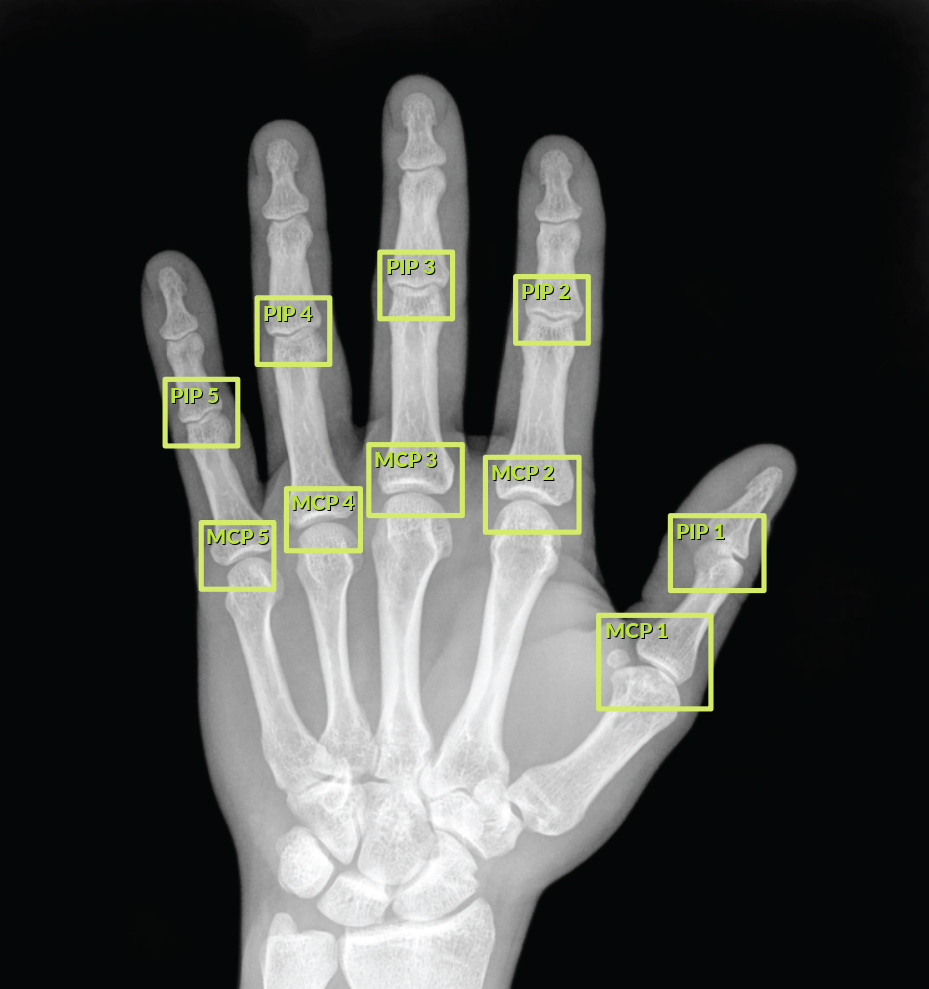
\includegraphics[width=\linewidth]{pics/xray-left-hand-annotated.png}
    \caption{Röntgenbild einer linken Hand mit markierten Metacarpophalangealgelenken (MCP) und proximalen Interphalangealgelenken (PIP), Quelle: \textit{OpenStax Anatomy and Physiology}, gefunden unter \url{https://commons.wikimedia.org/wiki/File:01_16_X-ray_of_Hand.jpg} (Lizenz: CC BY 4.0); Beschriftungen d.A.}
    \label{fig:xray-left-hand-annotated}
\end{figure}

Mit dem trainierten, validierten und erfolgreich getesteten Modell und dem dazu publizierten Fachartikel \textit{Bone Erosion Scoring for Rheumatoid Arthritis with Deep Convolutional Neural Networks}, \cite{rohrbach2019} ist der wissenschaftliche Grundstein für den produktiven Einsatz der automatischen Bewertung von Gelenken gemäss der Ratingen-Score gelegt. Bis dahin gibt es aber noch Einiges zu tun: Die erstellten Modelle müssen über einen Webservice zur Verfügung gestellt werden, damit sie in der Forschung zum Einsatz kommen können. Diese Aufgabe ist Gegenstand der vorliegenden Bachelorarbeit.

Geht es in der erwähnten Publikation \cite{rohrbach2019} v.a. um die Aspekte des Scorings im Bereich Machine Learning, liegt der Schwerpunkt in dieser Folgearbeit im Engineering-Bereich. Zunächst müssen die erstellten Modelle zu einer Software kombiniert werden, die als Web-Anwendung ansprechbar ist. Weiter muss sichergestellt werden, dass das automatische Scoring in nützlicher Frist durchgeführt werden kann ‒ gerade wenn das System unter hoher Last steht. Hierzu empfiehlt sich die Parallelisierung des Vorgangs: Die Röntgenbilder werden auf verschiedene Ausführungseinheiten verteilt. Dort wird das dargestellte Körperteil erkannt, es werden die relevanten Gelenke extrahiert und auf der Ratingen-Skala gescored. Am Schluss werden die ermittelten Scores als Gesamtergebnis zurückgeliefert.

Zudem sollen die Machine-Learning-Modelle austauschbar gemacht werden, sodass Verbesserungen auf diesem Gebiet schnell und einfach in den Produktivbetrieb einfliessen können. Hierbei ist es wichtig, dass die Qualität und Leistungsfähigkeit verschiedener Versionen miteinander verglichen werden können.

Das Ergebnis der Arbeit soll ein Prototyp für einen Webservice sein, der in bestehende Software eingebunden werden kann, um so ein automatisiertes, schnelles und präzises Scoring von Gelenken zu ermöglichen. Dadurch soll der Krankheitsverlauf von rheumatoider Arthritis besser nachverfolgt werden können, was etwa bei der Durchführung von Medikamentenstudien hilfreich sein kann.

\subsection{Projektauftrag}
\label{sec:projektauftrag}

Ziel der Arbeit ist es, den \textit{Proof of Concept}, der für die wissenschaftliche Publikation erstellt worden ist \cite{rohrbach2019}, für die Anwendung in der Praxis tauglich zu machen. Auf Basis der bestehenden Modelle, bzw. auf Basis des Codes zum Erstellen derselben, ist ein Deployment zu entwerfen und umzusetzen, das den Anforderungen des produktiven Betriebs genügt.

Die bestehenden Modelle sind in verschiedenen Versionen von TensorFlow umgesetzt worden. Zwar sollen die Modelle im Rahmen der vorliegenden Arbeit nicht auf eine aktuelle Version von TensorFlow migriert werden, es soll aber Teil der Arbeit sein, aufzuzeigen, was hierzu nötig wäre.

\subsubsection{Vorgaben}

Sämtliche Modelle, die für das Scoring eines Röntgenbildes benötigt werden, sind gegeben und vortrainiert. Sie erfüllen Minimum-Standars was ihre Performance betrifft.

\subsubsection{Erwartetes Resultat}
\label{sec:erwartetes-resultat}

Neben den für jede Bachelorarbeit zwingenden Resultate ‒ Schlussbericht (vorliegendes Dokument), Zwischen- und Schlusspräsentation, Web-Abstract, Einführungsvideo ‒ werden folgende Resultate vom Projekt erwartet:

\begin{enumerate}
    \item Stand der Technik zur Industrialisierung (Evaluation, Testing) von ML-Modellen
    \item Vorschlag für ein generisches Format von Modellen zum Exportieren aus ML-Frame\-works und zum Importieren zur Ausführung
    \item Vorschlag für geeignete Metriken zum Vergleich von Modellen
    \item Aufzeigen, was für eine Vereinheitlichung der Codebasis gemacht werden muss
    \item Lauffähiger Protoyp
    \begin{enumerate}
        \item Automatisierte Evaluation und Testing von neuen Modellen mit Vergleich zu alten Modellen und Minimum-Standards
        \item Visualisierung und Reporting der Performanz neuer Modelle
        \item API zum Ausführen des Modelles (Verteilen über mehrere GPUs)
        \item Load Balancing, Messaging Systems
        \item Nahtloses Austauschen von alten Modellen mit neuen Versionen
    \end{enumerate}
\end{enumerate}

\subsubsection{Abgrenzung}

Das Trainieren der Modelle ist nicht Teil der Arbeit. Die Modelle können als Blackbox betrachtet werden. Dementsprechend genügt es, sie aus einer High-Level-Sicht zu beschreiben.

Die effektive Integration in die Produktivumgebung von Seantis, sprich die Plattform \textit{HealthData.ai}\footnote{\url{https://www.healthdata.ai/en} (abgerufen am 27.05.2020)}, ist nicht Teil der Arbeit. Die hierzu notwendigen Schritte sollen jedoch beschrieben werden.

\subsection{Projektrisiken}
\label{sec:projektrisiken}

Im Folgenden werden verschiedene Projektrisiken und mögiche Mitigationsmassnahmen für diese aufgelistet:

\begin{description}
    \item[Keine lauffähigen Modelle] Die verschiedenen Modelle wurden teils vor mehreren Jahren entwickelt und trainiert. Ob sie tatsächlich funktionieren, und ob die Modelldaten noch in einem konsistenten Zustand auffindbar sind, ist zu Beginn des Projekts nicht klar.
        \begin{description}
            \item[Risiko] Eines oder mehrere Modelle sind nicht funktionstüchtig oder gar verloren.
            \item[Mitigation] Anhand von bestehendem Quellcode kann versucht werden, die Modelle neu zu erstellen. Scheitert dies, müssten fehlende Modelle durch Platzhalter (Mocks) ersetzt werden, die Predictions und ein bestimmtes Laufzeitverhalten simulieren.
        \end{description}
    \item[Aktualisierung der Modelle] Die zugrundeliegenden Modelle sind teils schon etwas älter und in unterschiedlichen Versionen bzw. mit unterschiedlichen Frameworks entwickelt worden.
        \begin{description}
            \item[Risiko] Die Modelle können nicht mit aktuellen Versionen der zugrundeliegenden Frameworks importiert werden.
            \item[Mitigation] Die Modelle werden mittels geeigneter Massnahmen (Container, virtuelle Umgebung) isoliert, sodass sie in ihrer ursprünglichen «Trainigsumgebung» ausgeführt werden können.
        \end{description}
    \item[Schlechte Performance (Prediction)] Da verschiedene Modelle zum Einsatz kommen, die bisher nie dem produktiven Betrieb ausgesetzt gewesen sind, kann es sein, dass deren Performance im Bezug auf die Qualität der Predictions schlecht ist.
        \begin{description}
            \item[Risiko] Eines oder mehrere Modelle weisen eine schlechte Prediction-Performance auf.
            \item[Mitigation] Dieses Risiko muss getragen werden. Die Prediction-Performance des Gesamtsystems ist durch das schwächste Modell nach oben begrenzt.
        \end{description}
    \item[Schlechte Performance (Laufzeit)] Für ein Scoring eines Röntgenbildes sind verschiedene Modelle in mehreren Schritten involviert.
        \begin{description}
            \item[Risiko] Die Laufzeit-Performance könnte so schwach ausfallen, dass ein produktiver Betrieb dadurch inpraktikabel wird.
            \item[Mitigation] Mit geeigneten architektonischen Massnahmen (parallele Abarbeitung, Ausführung auf GPUs) kann die Laufzeit-Performance erhöht werden. Genügt dies nicht, muss auf ein synchrones Ansprechen des Gesamtsystems zugunsten einer anderen, d.h. asynchronen Lösung verzichtet werden.
        \end{description}
    \item[Hoher Arbeitsspeicherverbrauch] Da mehrere Modelle für das Scoring eines Röntgenbildes benötigt werden, kann dies zu einem hohen Arbeitsspeicherverbrauch führen.
        \begin{description}
            \item[Risiko] Die Modelle und ihre umgebende Laufzeitumgebung können nicht gleichzeitig in den Arbeitsspeicher  eines Systems geladen werden.
            \item[Mitigation] Der Prototyp kann auf einem stärker bestückten System (etwa bei einem Cloud-Anbieter) ausgeführt oder über mehrere Systeme verteilt werden.
        \end{description}
\end{description}

\newpage

\section{Stand der Praxis, Forschung und Technik}

In diesem Kapitel geht es um den gegenwärtigen Stand der Praxis, der Forschung und der Technik.

Im Praxisteil werden die bereits bestehenden Machine-Learning-Modelle (siehe \secref{sec:bestehende-modelle}) betrachtet und in ihrer Funktionsweise beschrieben.

Was die Forschung betrifft, werden Metriken zur Evaluation von Machine-Learning-Modellen vorgestellt und dabei im Bezug auf ihre Eignung für das vorliegende Problem besprochen (siehe \secref{sec:evaluationsmetriken}).

Der Technikteil umfasst für diese Arbeit im Engineering-Bereich mehrere Themen: Zunächst soll untersucht werden, was mit dem Begriff des Webservices genau gemeint ist (siehe \secref{sec:web-services}). Anschliessend wird auf verschiedene Varianten eingegangen, wie verschiedene Komponenten zu einem funktionierenden Gesamtsystem kombiniert werden können (siehe \secref{sec:integrationsvarianten}). Konkrete Vorschläge für eine Systemarchitektur werden auf dieser Basis erst im Folgekapitel (siehe \secref{sec:architekturvarianten}) besprochen. Zum Schluss werden verschiedene Formate für Machine-Learning-Modelle untersucht und bewertet (siehe \secref{sec:modellformate}).

\subsection{Bestehende Modelle}
\label{sec:bestehende-modelle}

Für das Ermitteln der Ratingen-Score anhand eines Röntgenbildes sind mehrere Schritte nötig.

Zunächst muss das auf dem Röntgenbild abgebildete Körperteil erkannt werden. Hierfür ist das Modell \texttt{body\_part} zuständig.\footnote{Die Namen der Modelle in diesem und in den weiteren Kapiteln wurden der Verzeichnisstruktur entnommen, in der die entsprechenden Daten abgelegt worden waren.} Dieses Modell kann verschiedene Körperteile erkennen, u.a. Hände, Füsse (jeweils mit links/rechts-Unterscheidung) und Becken.

Im nächsten Schritt werden aus dem Röntgenbild die relevanten Gelenke extrahiert. Das Modell (bzw. die Modellsammlung) \texttt{joint\_detection} kann neben den proximalen Interphalangealgelenken (PIP) und den Metacarpophalangealgelenken (MCP) auch das Karpalgelenk (vulgo: «Handgelenk») auf einem Röntgenbild erkennen und extrahieren.

Im dritten und letzten Schritt wird das Scoring für ein bestimmtes Gelenk auf einem entsprechenden Bildausschnitt vorgenommen. Hierfür ist das Modell \texttt{ratingen\_score} zuständig.\footnote{Dieser Name wurde nicht anhand einer Verzeichnisstruktur, sondern anhand der Funktionalität des Modells ausgesucht.} Dieses Modell unterstützt nur das Scoring der PIP- und MCP-Gelenke der linken Hand.

Die Menge der möglichen Inputs wird somit in dieser Kette von Modellen wie ein Trichter verengt: Können zu Beginn Hände, Füsse, Becken usw. erkannt werden, ist das Scoring am Schluss nur für zehn Gelenke (PIP 1-5 und MCP 1-5) der linken Hand möglich. 

Dadurch verkommt das recht mächtige Modell \texttt{body\_part} im Rahmen dieser Arbeit zu einer blossen Validierungsengine: Zeigt das Röntgenbild eine linke Hand? Wenn ja, kann der Prozess weitergeführt werden. Wenn nein, kann auf weitere Schritte verzichtet werden, denn ein Scoring wird damit nicht funktionieren.\footnote{Rein technisch könnten erkannte rechte Hände gespiegelt und an die Extraktion weitergeleitet werden. Auch wäre es möglich, etwa Röntgenbilder von Füssen an die Extraktion weiterzuleiten, in der Hoffnung, darauf entsprechende Gelenke zu erkennen. Solche Versuche sollen im Rahmen dieser Arbeit kategorisch unterlassen werden, da das Modell \texttt{ratingen\_score} ausschliesslich mit Gelenken von linken Händen trainiert, evaluiert und getestet worden ist.} Diese Restriktion kann möglicherweise zu einem späteren Zeitpunkt aufgehoben werden, sollten die Downstream-Modelle \texttt{joint\_extraction} und \texttt{ratingen\_score} entsprechend erweitert werden.

\subsubsection{Erkennung von Körperteilen: \texttt{body\_part}}
\label{sec:modell-body-part}

Das Modell \texttt{body\_part} kann, wie bereits beschrieben, auf Röntgenbildern verschiedene Körperteile erkennen. Im Kontext dieser Arbeit ist jedoch nur relevant, ob ein Röntgenbild (Input) eine linke Hand darstellt oder nicht.

Der Input für das Modell ist eine Liste monochromer Bilder von 144 mal 144 Pixeln. Technisch gesprochen ist dies ein NumPy-Array mit der Dimension \texttt{(n, 144, 144, 1)}, wobei \texttt{n} für die Anzahl der Bilder in der Liste steht.

Im Code zum Trainieren des Modells werden verschiedene Röntgenbilder zunächst auf die entsprechende Auflösung reduziert, d.h. gestaucht. Dieser Schritt ist für den produktiven Einsatz mit Sicherheit nötig, soll der Benutzer Bilder in verschiedenen Auflösungen verwenden können. Eine Seitenverhältnis von 1:1 (quadratische Form) dürfte dabei hilfreich sein, da das Bild ansonsten gestaucht werden muss.

Der Output des Modells ist eine Liste von Wahrscheinlichkeiten ‒ bzw. eine Liste davon, denn für \texttt{n>1} werden mehrere Bilder in einem Prediction-Schritt verarbeitet. Die innere Liste ist ein NumPy-Array mit Fliesskommazahlen im Bereich $[0..1]$. Diese beschreiben, mit welcher Wahrscheinlichkeit ein Bild ein bestimmtes Körperteil zeigt.

Da im Rahmen der vorliegenden Arbeit nur linke Hände von Belang sind, kann das Element mit dem Index 6 (\texttt{left hand} in der Label Map) extrahiert werden. Ein bestimmter Threshold für die Wahrschienlichkeit könnte nachgelagert geprüft werden.

Das Modell wurde mit den Libraries \texttt{tensorflow} (Version 0.12.1) und \texttt{tflearn} (Version 0.2.1) erstellt und im \texttt{tflearn}-Format abgespeichert. Weiter kommt \texttt{scikit-image} in einer dazu kompatiblen Version zum Einsatz. Es ist mit einem Docker-Image basierend auf dem Image \texttt{python:3.6} lauffähig.

\subsubsection{Extraktion von Gelenken: \texttt{joint\_detection}}
\label{sec:modell-joint-detection}

Wie in der Kapitelanleitung bereits erwähnt, handelt es sich bei \texttt{joint\_detection} um eine ganze Reihe von Modellen, elf an der Zahl: für die zehn Gelenke MCP 1-5 und PIP 1-5, sowie für das Karpalgelenk (Handgelenk). Letzteres ist für die vorliegende Arbeit nicht relevant.

Das Modell extrahiert aus einem Röntgenbild (JPEG-Format), welches über das Dateisystem zur Verfügung gestellt wird, ein bestimmtes Gelenk. Der Gelenkname muss dabei als Parameter mitgegeben werden, z.B. \texttt{mcp3} oder \texttt{pip5}. Der Output ist eine JPEG-Datei der Grösse 150 mal 150 Pixel.\footnote{Strenggenommen hat das Modell zwei Outputs: erstens eine Reihe sogenannter \textit{Boxes}, die je durch vier Gleitkommazahlen definiert sind; zweitens eine Reihe von \textit{Confidences}, bestehend aus je zwei Gleitkommazahlen. Auf die genaue Bedeutung dieser Werte soll hier nicht weiter eingegangen werden, zumal die Modelle nur aus einer High-Level-Sicht zu beschreiben sind (siehe \secref{sec:erwartetes-resultat}). Diese Boxes und Confidences könnten evtl. später auch dazu verwendet werden, die detektieren und gescorten Gelenke auf dem Bild grafisch hervorzuheben (siehe \secref{sec:weitere-ideen}).}

Es wird somit pro Gelenk eine Datei extrahiert. Hierbei fällt auf, dass das Upstream-Modell \texttt{body\_part} mit Bildern von 144 mal 144 Pixeln für das ganze Röntgenbild arbeitet, während in den \texttt{joint\_detection}-Modellen jedes der zehn zu detektierenden Elemente mit einer Auflösung von 150 mal 150 Pixeln ausgegeben wird. Der initiale Bild-Input sollte also möglichst hochauflösend sein.

Die \texttt{joint\_detection}-Modelle wurden ebenfalls mit \texttt{tensorflow} Version 0.12.1 erstellt und im \texttt{tflearn}-Format abgelegt. Als weitere Libraries kommen \texttt{Pillow} (Version 3.4.2) und \texttt{scipy} (Version 0.18.1) zum Einsatz. Das verwendete Docker-Image basiert wiederum auf dem Image \texttt{python:3.6}.

\subsubsection{Scoring von Gelenken: \texttt{ratingen\_score}}
\label{sec:modell-ratingen-score}

Das Modell \texttt{ratingen\_score}, welches für das eigentliche Scoring zuständig ist, wurde nicht bei Seantis entwickelt, sondern im Rahmen einer Bachelorarbeit \cite{rohrbach2017}. Es ordnet einem extrahierten Bild eines Gelenkes eine Score von 0 bis 5 zu. Ein gesundes Gelenk hat die Score 0. Ein Gelenk mit der Score 1 weist eine Gewebeerosion von maximal 20\% auf. Jede höhere Score deckt einen weiteren Bereich von 20\% ab, sodass eine Score von 5 einer Erosion von 80\% bis 100\% gleichkommt \cite[S. 10]{rohrbach2017}.\footnote{Gelenke mit einer derart starken Schädigung machten einen extrem geringen Teil des Trainingssets aus. Das Problem ist nicht etwa, dass es keine solchen Fälle mit beinahe komplett erodiertem Gelenkgewebe gebe, sondern weil betreffende Patienten kaum ihre Hand flach ausbreiten können, sodass derart erodierte Gelenke auf den Röntgenbildern praktisch nicht auszumachen sind.}

Neben der Ratingen-Score gibt es noch eine weitere Score: die Rau-Score. Beschreibt die Ratingen-Score die Schädigung eines bestimmten Gelenkes, geht es bei der Rau-Score um eine umfassendere Einschätzung: Neben den zehn MCP- und PIP-Gelenken beider Hände werden auch die Karpalgelenke beider Hände sowie fünf Gelenke beider Füsse berücksichtigt. Janick Rohrbach hat das Berechnen dieser Score in seiner Bachelorarbeit beschrieben \cite[S. 10]{rohrbach2017}.

Als Input nimmt das Modell ein NumPy-Array bestehend aus einem oder mehreren RGB-Bildern mit der Auflösung 150 mal 150 Pixel entgegen. Technisch gesprochen sind dies NumPy-Arrays mit der Dimension \texttt{(n, 150, 150, 3)}, wobei \texttt{n} für die Anzahl Bilder steht.

Der Output ist ein NumPy-Array, bei dem jeder Eintrag die Wahrscheinlichkeit für eine bestimmte Score eines Gelenkbildes repräsentiert. So wäre beispielsweise \texttt{[0.68 0.21 0.08 0.02 0.01 0.00]} ein Eintrag mit der Score 0 (höchste Wahrscheinlichkeit), ein Output wie \texttt{[0. 0.12 0.73 0.15 0. 0.]} stünde für einen Eintrag mit der Score 2.

Das Modell wurde mit einer neueren Version von TensorFlow (1.4.0) erstellt. Weitere zur Ausführung benötigte Libraries sind \texttt{pandas}, \texttt{Pillow}, \texttt{h5py}, \texttt{scikit-learn} und \texttt{keras-utils}. Abgespeichert ist es im \texttt{.h5}-Format. Es basiert auf dem Inception-V3-Modell von François Chollet.\footnote{\url{https://github.com/fchollet/deep-learning-models} (abgerufen am 01.05.2020)}

Im Gegensatz zu den bisher beschriebenen Modellen musste das Scoring-Modell neu trainiert werden, da die Modelldaten weder bei Seantis noch auf dem GitHub-Repository\footnote{\url{https://github.com/janickrohrbach/arthritis-net} (abgerufen am 01.05.2020)} der Bachelorarbeit von Janick Rohrbach vorhanden waren. Da auf dem GPU-Server von Seantis (\texttt{perses.seantis.ch}) eine ältere Python-Version (3.5) im Einsatz ist, wurde diese Version auch für den Container verwendet, in dem das Modell ausführbar ist. Da das Scoring-Modell aus technischen Gründen\footnote{CUDA war nach dem Aktualisieren des Grafikkartentreibers nicht mehr funktionstüchtig und erforderte einen Neustart des Servers. Aufgrund einer darauf eingerichteten Volume-Verschlüsselung kann ein solcher Neustart nur vor Ort durchgeführt werden, was aufgrund von verordnetem Home-Office (Covid-19-Krise) nicht sofort möglich war. Nach einem Neustart vor Ort funktionierte CUDA wieder einwandfrei.} nicht auf dem Systsem von Seantis zu Ende trainiert werden konnte, wurde eine GPU-Instanz bei Exoscale verwendet, auf welcher die Linux-Distribution Debian Stretch installiert ist. Aus diesem Grund dient \texttt{python:3.5-stretch} als Base-Image für die Ausführung des Scoring-Modells.

\subsection{Webservices}
\label{sec:web-services}

Der zu erstellende Prototyp soll als Webservice umgesetzt werden (siehe Kapitel \secref{sec:Problemstellung}). Für den Begriff \textit{Webservice} gibt es verschiedene Definitionen, wovon hier drei exemplarisch erwähnt sind ‒ in der Reihenfolge, in der sie bei der Google-Suche nach «Definition Web Service» beim Autor erschienen sind:

\begin{enumerate}
\item \say{\textit{A web service is an application or data source that is accessible via a standard web protocol (HTTP or HTTPS). Unlike web applications, web services are designed to communicate with other programs, rather than directly with users.\footnote{Ein Webservice ist eine Applikation oder Datenquelle, die über Standard-Web-Protokolle (HTTP oder HTTPS) erreichbar ist. Im Gegensaz zu Web-Anwendungen sind Webservices dafür ausgelegt mit anderen Programmen zu kommunizieren, nicht direkt mit den Benutzern. (Übersetzung des Autors)}}} \cite{techterms-webservice}
\item \say{\textit{A Web service is a software service used to communicate between two devices on a network. More specifically, a Web service is a software application with a standardized way of providing interoperability between disparate applications. It does so over HTTP using technologies such as XML, SOAP, WSDL, and UDDI.\footnote{Ein Webservice ist ein Software-Service, der verwendet wird um zwischen zwei Geräten in einem Netzwerk zu kommunizieren. Genauer gesagt ist ein Webservice eine Software-Anwendung mit einer standardisierten Art um Interoperabilität zwischen verschiedenartigen Anwendungen anzubieten. Dies wird über HTTP mithilfe von Technologien wie XML, SOAP, WSDL und UDDI erreicht. (Übersetzung des Autors)}}} \cite{techopedia-webservice}
\item \say{\textit{Il s'agit d'une technologie permettant à des applications de dialoguer à distance via Internet, et ceci indépendamment des plates-formes et des langages sur lesquelles elles reposent. Pour ce faire, les services Web s'appuient sur un ensemble de protocoles Internet très répandus (XML, HTTP), afin de communiquer. Cette communication est basée sur le principe de demandes et réponses, effectuées avec des messages XML.\footnote{Es handelt sich um eine Technologie, die es Anwendungen ermöglicht über das Internet zu kommunizieren, und zwar unabhängig von Plattformen und Sprachen, auf denen sie basieren. Um dies zu erreichen, stützen sich Webservices auf eine Menge weit verbreiteter Internet-Protokolle (XML, HTTP) für die Kommunikation. Diese Kommunikation basiert auf dem Anfrage-Antwort-Prinzip, was mithilfe von XML-Nachrichten bewerkstelligt wird. (Übersetzung des Autors)}}} \cite{les-services-web}
\end{enumerate}

Die Auflistung könnte beliebig weitergeführt werden. Allen Definitionen ist gemeinsam, dass HTTP(S) als Protokoll verwendet wird. Erwähnte Technologien wie XML und SOAP sind dabei schon länger auf dem Rückzug und werden zusehends von REST und JSON verdrängt \cite{infoq-soap-rest}.

Für den zu erstellenden Protoyp soll somit eine RESTful-API (via HTTP) angeboten werden. Genauer soll der Protoyp \textit{gegen aussen} eine RESTful-API anbieten. Ob REST auch für die interne Kommunikation zwischen den Komponenten (siehe \secref{sec:bestehende-modelle}) eine gute Wahl ist, soll in der Architekturdiskussion im Folgekapitel (siehe \secref{sec:architekturvarianten}) untersucht werden.

\subsection{Integrationsvarianten}
\label{sec:integrationsvarianten}

Die gängigsten Methoden zum Integrieren von Anwendungen sind \textit{File Transfer}, \textit{Shared Database}, \textit{Remote Procedure Invocation} und \textit{Messaging} \cite[Introduction, S. xxx]{enterprise-integration-patterns} ‒ und, ergänzend wie gerade besprochen, RESTful-APIs.\footnote{Der Begriff REST und das Konzept der RESTful-APIs sind zwar spätestens seit dem Jahr 2000 bekannt \cite[Kapitel 6]{fielding2000}. Weite Verbreitung fand das Konzept jedoch erst später, gerade mit dem Siegeszug von \textit{Microservices} ‒ ein Begriff, der erst seit dem Jahr 2011 geläufig ist \cite{leanix-microservices}. RESTful-APIs waren beim Erscheinen des erwähten Standardwerks im Jahr 2004 zwar schon bekannt, aber nicht weit verbreitet.} Aufgrund des synchronen Modus können REST und HTTP in diesem Kontext am ehesten mit Remote Procedure Invocation (RPC) verglichen werden, wobei HTTP an Ressourcen und RPC an Funktionen orientiert ist.

Die genannten Arten der Integration bauten aufeinander auf und stellten jeweils eine Verbesserung gegenüber ihrem Vorgänger dar, was jedoch jeweils eine erhöhte Komplexität zur Folge habe \cite[S. 41-42]{enterprise-integration-patterns}. Die einfachste Variante sei der Verzicht auf eine Integration von Anwendungen, indem man sich auf eine einzelne, zusammenhängende (d.h. monolithische) Applikation beschränkt, die gar keine Integration erfordert \cite[S. 39]{enterprise-integration-patterns}. Dies ist oftmals nicht möglich oder nicht sinnvoll, wie z.B. im vorliegenden Projekt, bei dem zueinander inkompatible Laufzeitumgebungen zum Einsatz kommen, die sich nicht in eine monolithische Applikation zwängen lassen. 

Die Vor- und Nachteile der genannten Integrationsvarianten lassen sich folgendermassen zusammenfassen:

\begin{description}
    \item[File Transfer] Die Dateiübertragung sei die wohl einfachste Integrationsvariante, denn praktisch alle Betriebssysteme unterstützten Dateien und deren Austausch mit anderen Systemen oder Prozessen. Diese Einfachheit bezahle der Entwickler jedoch damit, dass er sich um viele Aspekte der Integration selber kümmern muss: Konventionen für Dateinamen und Verzeichnisse und das Sicherstellen deren Eindeutigkeit; das Löschen alter Dateien und das Feststellen für dessen Notwendigkeit; Sperrmechanismen zum Sicherstellen, dass nicht zwei Anwendungen gleichzeitig auf eine Datei zugreifen; Übertragung der Dateien über ein geeignetes Protokoll auf ein passendes Medium. Ein Hauptproblem stellten dabei die verschiedenen Bedürfnisse der beteiligten Anwendungen für die Synchronisierung der Dateien dar: Manche Applikationen benötigten Aktualisierungen in Sekundenschnelle, während für andere eine nächtliche, wöchentliche oder monatliche Aktualisierung ausreiche. Solche Unterschiede könnten oft zu Inkonsistenzen führen, die sich desto schwerer beheben liessen, je weiter ihr Auftreten von ihrer Kenntnissnahme entfernt sei. \cite[S. 43-46]{enterprise-integration-patterns}
    \item[Shared Database] Gegenüber der Dateiübertragung biete eine gemeinsame Datenbank einige Vorteile. Zeitliche Lücken träten kaum mehr auf, denn jede Applikation habe stets Zugriff auf den aktuellen Stand. Mithilfe einer Datenbank sei es zudem einfacher, ein bestimmtes Datenformat sicherzustellen. Dank des Transaktionssystems von Datenbanksystemen seien die Daten stets konsistent. Zwar müsse man viel Aufwand betreiben, um bei den verschiedenen Applikationen mit gleicher Datenbank ein Schema auszuarbeiten, mit dem alle Applikationen umgehen können; es sei jedoch besser, diese Probleme direkt anzugehen, statt  ihnen auszuweichen, um sich in der anschliessenden Integrationsphase wieder davon einholen zu lassen. Alle beteiligten Applikationen auf einen gemeinsamen Nenner zu bringen sei jedoch manchmal so schwierig, dass das Ergebnis dieser Übung unbefriedigend ausfalle, und in einem Datenschema resultiere, mit dem nur schwer umzugehen ist. Solche Konflikte könnten dazu führen, dass sich Trennungen aufdrängten.\footnote{Siehe auch Conway's Law: \textit{«Any organization that designs a system (defined broadly) will produce a design whose structure is a copy of the organization's communication structure.»} \cite{conway1968committees}} Der Zugriff von mehreren Applikationen auf eine gemeinsame Datenbank mit dem damit einhergehenden wiederholten Lesen und Schreiben der gleichen Daten könne dazu führen, dass die Datenbank zum Flaschenhals werde, oder dabei gar Deadlocks aufträten. \cite[S. 47-49]{enterprise-integration-patterns}
    \item[Remote Procedure Invocation] Die beiden genannten Ansätze \textit{File Transfer} und \textit{Shared Database} haben gemeinsam, dass sie Daten verschiedener Applikationen integrieren, nicht aber deren Funktionalität. \cite[S. 49]{enterprise-integration-patterns} Einer der mächtigsten Mechanismen zur Strukturierung von Software sei die Kapselung mittels Funktionen. Mittels \textit{Remote Prodecure Invocation} (RPI) oder \textit{Remote Procedure Call} (RPC) könnten auch zwischen Applikationen Funktionen aufgerufen werden. Daten werden dabei als Funktionsparameter übertragen. Die internen Datenstrukturen der einzelnen Applikationen können dabei frei gestaltet und zu einem späteren Zeitpunkt verändert werden, ohne dass eine andere Applikation davon betroffen sei. Weiter könnten Anwendungen mittels RPI mehrere Schnittstellen auf die gleichen Daten anbieten.\footnote{Dies ist eine Ähnlichkeit zu HTTP, das verschiedene Methoden (\texttt{GET}, \texttt{POST} usw.) bietet, um auf die gleichen Ressourcen zuzugreifen.} Der Funktionsaufruf sei ein für alle Programmierer geläufiges Modell, was einerseits ein Vorteil ist, andererseits problematisch sein kann, zumal sich die Performance zwischen einem lokalen und einem entfernten Funktionsaufruf um mehrere Grössenordnungen unterscheiden kann. Ausserdem verleitet RPI dazu, eine verteilte Applikation wie eine einzelne, zusammenhängende zu gestalten, was zu einer engen Kopplung führe, sich aber angesichts der Performanceeinbussen nicht so anfühle. \cite[S. 50-52]{enterprise-integration-patterns}
    \item[Messaging] Die grösste Herausforderung bei der Integration von Anwendungen bestehe oft darin, den Zeitverlust beim Austausch zwischen Systemen so gering wie möglich zu halten, ohne die Anwendungen dabei eng aneinander zu koppeln, oder dabei die Weiterentwicklung oder das Laufzeitverhalten der Anwendungen zu beeinträchtigen. Hierzu benötige es einen ähnlichen Mechanismus wie \textit{File Transfer}, womit Datenpakete schnell produziert und einfach transferiert werden können ‒ und darüber hinaus den Empfänger informiere, dass ein Datenpaket zur Verarbeitung anstehe, sowie einen Retry-Mechanismus für gescheiterte Übertragungen biete. Im Gegensatz zur \textit{Shared Database} soll das interne Datenschema einer Anwendung veränderbar bleiben. Im Gegensatz zur \textit{Remote Procedure Invocation} soll die Übertragung asynchron ablaufen, sodass der Aufrufer nicht blockierend auf die Antwort warten muss. Weiter sollen auch Nachrichten verschickt werden können, ohne dass die Gegenseite zu dieser Zeit bereit sein muss. \textit{Messaging} erfülle alle diese Anforderungen, und biete darüber hinaus noch verschiedene Verteilungsmechanismen wie Broadcasting zu allen oder Routing zu verschiedenen Empfängern, oder verschiedene Topologien. Da Nachrichten zeitnah verarbeitet werden können, fallen die Synchronisationsprobleme von \textit{File Transfer} weg. Diese Vorteile erkaufe sich der Entwickler mit einer steilen Lernkurve und einer Reihe neuer Herausforderungen, von denen der Rest des Buches grösstenteils handelt. \cite[S. 53-59]{enterprise-integration-patterns}
\end{description}

\textit{Messaging} ist somit die mächtigste, aber auch komplizierteste Variante. Wie sich die beschriebenen Machine-Learning Modelle (siehe \secref{sec:bestehende-modelle}) integrieren lassen, ist Thema des nächsten Kapitels (siehe \secref{sec:architekturvarianten}).

\subsection{Evaluation von Modellen}
\label{sec:evaluation-von-modellen}

Der Projektauftrag erwähnt den \textit{Vorschlag für geeignete Metriken zu Vergleich von Modellen} als erwartetes Resultat (siehe \secref{sec:erwartetes-resultat}). Hierbei soll es nicht um die Evaluation der einzelnen verwendeten Modelle gehen, sondern um eine Evaluation des Gesamtsystems, das zu diesem Zweck wie ein grosses, zusammenhängendes Modell betrachtet wird. Zu einem späteren Zeitpunkt, an dem einzelne, verbesserte Modelle in das System einfliessen, können verschiedene Versionen des Gesamtsystems im Bezug auf ihre Performance miteinander verglichen werden.

\subsubsection{Verschiedene Datentypen}
\label{sec:verschiedene-datentypen}

Um eine passende Art der Evaluation zu finden, muss man sich zuerst vergegenwärtigen, mit welcher Art von Prediction (Output) man es zu tun hat. Hierbei fällt auf, dass in Wissenschaft und Praxis von verschiedenen Arten von Daten die Rede ist.

Einen guten Überblick über die Thematik bietet der Artikel \textit{7 Data Types: A Better Way to Think about Data Types for Machine Learning} \cite{7-data-types}. So werde im Machine-Learning-Bereich teilweise nur zwischen numerischen und kategorischen Daten unterschieden. Diese Unterscheidung greife aber zu kurz und lasse sich weiter verfeinern und erweitern. Die elf [sic.\footnote{Die ursprünglichen sieben Datentypen wurden in einer späteren Version des Artikels um vier weitere ergänzt.}] Datentypen lassen sich folgendermassen zusammenfassen:

\begin{description}
    \item[Useless] Daten, oft zufällige und eindeutige wie z.B. eine Kontonummer, die zwar als Identifikation von Datensätzen, aber nicht zum Trainieren eines Modells verwendet werden können.
    \item[Nominal] Diskrete Werte ohne numerische Beziehung zwischen den Werten, wie z.B. Arten von Tieren, auf die sich keine statistischen Operationen wie mean und median anwenden lassen.
    \item[Ordinal] Diskrete Werte, die rangiert und sortiert werden können, wobei der Abstand zwischen zwei Zahlen unbekannt ist.
    \item[Binary] Diskrete Werte, welche in die beiden Kategorien null und eins eingeteilt werden können, und so einen Spezialfall von Nominal-, Ordinal- und/oder Intervalldaten darstellen.
    \item[Count] Diskrete, positive Zahlen, die eine Anzahl wiedergeben, und auf die statistische Operationen wie mean und median sinnvollerweise angewendet werden können.
    \item[Time] Zyklische, sich wiederholende, kontinuierliche Daten, die sich auf verschiedene Perioden (Jahr, Monat, Tag usw.) beziehen können.
    \item[Interval] Daten, bei denen benachbarte Zahlen die gleichen Abstände voneinander haben, aber kein zeitliches Muster repräsentieren.
    \item[Image] Zweidimensionale Bilder, wie z.B. Röntgenbilder.
\end{description}

Die drei weiteren vorgeschlagenen Kategorien, die für die vorliegende Arbeit nicht releant sind, lauten: Video, Audio und Text.

\subsubsection{Datentypen der Modelle}

Bei den verschiedenen Modellen kommen unterschiedliche Arten von Daten zum Einsatz. Die Einteilung nach der gerade aufgestellten Taxonomie ist dabei nicht immer klar und eindeutig:

\begin{description}
    \item[\texttt{body\_part}] Für ein Röntgenbild wird eine Reihe von Wahrscheinlichkeiten erstellt, die beschreiben, welche Art von Körperteil es abbildet. Hierbei handelt es sich um Intervalldaten, denn eine Wahrscheinlichkeit von 0.8 kann als doppelt so wahrscheinlich wie eine Wahrscheinlichkeit von 0.4 interpretiert werden. Für die vorliegende Arbeit ist jedoch nur ein Körperteil (die linke Hand) und somit nur deren Wahrscheinlichkeit relevant (siehe \secref{sec:modell-body-part}), welche mithilfe eines passenden Schwellenwertes zu einer Binärklassifikation regrediert. Ob die Interpretation der Prediction anhand dieses Schwellenwerts Teil der Modellkomponente oder zu den Aufgaben des Aufrufers gehört, oder gar weggelassen werden kann, ist eine Architekturfrage.
    \item[\texttt{joint\_detection}] Aus einem Röntgenbild einer linken Hand werden bis zu zehn Gelenke extrahiert. Sowohl Input wie Output sind Bilddaten. Für die Evaluation des Modells sind Bilddaten jedoch ungeeignet, da die Definition der Testdaten und der Vergleich mit den Predictions aufwändig (Vergleich von 2D-Matritzen) und fehleranfällig (Verschiebung um einzelne Pixel) ist. Für die Evaluation ist es sinnvoller, die Frage zu stellen, ob ein betreffendes Gelenk (PIP 1, MCP 3, usw.) gefunden worden ist oder nicht, was mit einer Binärklassifikation pro Gelenk bewerkstelligt werden kann. Da pro Bild zehn Gelenke gefunden oder nicht gefunden werden können, ist eine Zählung (Count) im Bereich null bis zehn der geeignete Datentyp, sofern die zehn Extraktionsvorgänge konzeptuell als ein übergeordneter Vorgang betrachtet werden sollen.
    \item[\texttt{ratingen\_score}] Bei der Ratingen-Score handelt es sich um Intervalldaten von null bis hundert Prozent. In der SCQM-Datenbank werden die einzelnen Gelenkscores als Anteil des geschädigten Gelenkgewebes mit diskreten Prozentzahlen und einer Auflösung von 5\% abgespeichert. Das entsprechende Modell teilt diese Score jedoch in sechs Kategorien ein, wobei die Kategorien 1 bis 5 jeweils für eine Bandbreite von 20\% stehen. Ein Spezielfall ist die Kategorie 0, die für ein gesundes Gelenk mit 0\% Erosion steht. Die Prediction hat damit sowohl Aspekte einer nominalen Kategorisierung als auch von Intervalldaten. Durch die Vermischung der Nominalzahl (Kategorie 0) mit Intervalldaten (Kategorien 1-5) liegen unterschiedlich grosse Abstände zwischen den Kategorien vor, wodurch die Kategorien als Ordinalzahlen betrachtet werden können. Für die Evaluation des Gesamtsystems ist weiter zu beachten, dass pro Vorgang nicht nur eines, sondern (bis zu) zehn Gelenke gescored werden. Die Anzahl der Übereinstimmungen von Prediction und tatsächlichem Wert könnten gezählt werden, also z.B. acht von zehn Gelenken wurden korrekt gescored. Besser ist eine Prozentangabe (Intervalldaten), welche die Anzahl der korrekt gescorten Gelenke der Anzahl vorhandener Gelenke gegenüberstellt, zumal diese Metrik auch bei fehlenden Gliedmassen oder unerkannten Gelenken eine sinnvolle Aussage macht.\footnote{Auf den Röntgenbildern sind statt Gelenke oftmals Metallgegenstände zu sehen, welche im fortgeschrittenen Krankheitsstadium eher als Ersatz denn als Reparatur eines Gelenks zu verstehen sind.}
\end{description}

Betrachtet man die drei Modelle als Gesamtsystem, besteht der Output aus einer Reihe (null bis zehn) Scores im Intervall $[0..5]$. Zwar sind für die Performance des Gesamtsystems alle drei Modelle ausschlaggebend, der Evaluation stehen jedoch nur die Scores des letzten Modells zur Verfügung.

Für die Evaluation des Gesamtsystems kann pro Vorgang (Röntgenbild) eine Menge von Ordinalzahlen (Output, $[0..5]$) mit einer Reihe von Intervalldaten (Testdaten, $[0..100]$) verglichen werden (im Sinne von \textit{Matching}), wobei auch die Grösse dieser Menge (Intervallzahl, $[0..10]$) aussagekräftig ist.

\subsubsection{Mögliche Evaluationsmetriken}
\label{sec:evaluationsmetriken}

Für die ermittelten Datentypen gibt es verschiedene Evaluationsmetriken. Die ermittelten Scores für die Gelenke eines oder mehrerer Vorgänge könnten zusammengefasst und auf ihre Genauigkeit (Accuracy) geprüft werden \cite[S. 8]{zheng2015}:

\begin{equation}
    $$ \text{Global Accuracy} = \frac{\text{Total Correct Predictions}}{\text{Total Predictions}} $$
    \caption{Global Accuracy}
    \label{equ:global-accuracy}
\end{equation}

Eine solche Klassifikation behandle jedoch alle Klassen gleich, was gerade in medizinischen Anwendungen oft problematisch sein könne, zumal \textit{false positives} (gesunden Patient als krank eingestuft) und \textit{false negatives} (kranken Patient als gesund eingestuft) oft stark unterschiedliche Konsequenzen hätten.\footnote{Da der zu erstellende Prototyp nicht in der Diagnostik, sondern für die langfristige Erforschung einer Krankheit eingesetzt wird, ist das genannte Problem für die vorliegende Arbeit weniger relevant.} Eine \textit{Confusion Matrix} schaffe hier Abhilfe, und wäre für die binäre Klassifikation und somit für das Modell \texttt{body\_part} eine sinnvolle Metrik.\footnote{Sofern die Interpretation eines Schwellenwerts Teil des Modells sein soll.} \cite[S. 8]{zheng2015}

Da bei der Evaluation des Gesamtsystems Scores von sechs verschiedenen Klassen relevant sind, und da die einzelnen Klassen mit stark unterschiedlicher Häufigkeit auftreten \cite[S. 16-17]{rohrbach2017}, ist die \textit{Per-Class Accuracy} eine weitere mögliche Metrik. Für Klassen mit kleinen Datenbeständen könne die Varianz jedoch sehr hoch ausfallen, und die Evaluation darum wenig aussagekräftig werden \cite[S. 9]{zheng2015}:

\begin{equation}
    $$ \text{Per-Class Accuracy}_{\text{Class n}} = \frac{\text{Correct Predictions}_\text{Class n}}{\text{Total Predictions}_\text{Class n}} $$
    \caption{Per-Class Accuracy}
    \label{equ:per-class-accuracy}
\end{equation}

Die Kosten von \textit{false positives} kommen mit der \textit{Precision} zum Tragen. Die Precision ist definiert als \cite{precision-recall-f1}:

\begin{equation}
    $$ \text{Precision}=\frac{\text{True Positive}}{\text{True Positive} + \text{False Positive}}$$
    \caption{Precision (berücksichtigt die Kosten von \textit{false positives})}
    \label{equ:precision}
\end{equation}

Möchte man die Kosten von \textit{false negatives} abbilden, ist der \textit{Recall} eine geeignete Metrik. Der Recall ist definiert als \cite{precision-recall-f1}:

\begin{equation}
$$ \text{Recall}=\frac{\text{True Positive}}{\text{True Positive} + \text{False Negative}} $$
    \caption{Recall (berücksichtigt die Kosten von \textit{false negatives})}
    \label{equ:recall}
\end{equation}

Die beiden Metriken Precision und Recall lassen sich mittels \textit{F1 Score} zu einer einzigen Metrik kombinieren, die gegenüber der Accuracy den Vorteil hat, dass sie die «Kosten» von \textit{false positives} und \textit{false negatives} berücksichtigt \cite{precision-recall-f1}:

\begin{equation}
    $$ \text{F1} = 2 \times \frac{\text{Precision} \times \text{Recall}}{\text{Precision} + \text{Recall}} $$
    \caption{F1 Score (bildet die Kosten von \textit{false positives} und \textit{false negatives} ab)}
    \label{equ:f1score}
\end{equation}

\textit{Log-Loss} ist eine Metrik, die sich bei der Klassifikation mit Wahrscheinlichkeiten einsetzen lässt. Ihr Vorteil gegenüber der einfachen \textit{Accuracy} bei der Binärklassifikation ist, dass sie \textit{near misses} («knapp daneben») weniger stark bestraft als grobe Abweichungen der Predictions vom eigentlichen Wert \cite[S. 9-10]{zheng2015}. Diese Metrik liesse sich sinnvollerweise zur Evaluation des Modells \texttt{body\_part} einsetzen (sofern dieses eine Wahrscheinlichkeit und keine interpretierte Binärklassifikation liefert), jedoch nicht für das Gesamtsystem.

Mithilfe einer \textit{AUC}-Metrik (\textit{Area under the curve}) liesse sich die Sensitivität eines Klassifikators grafisch aufzeigen, indem die Rate der \textit{true positives} zu der Rate der \textit{false positives} geplottet werde (\textit{ROC}-Kurve, \textit{receiver operating characteristic curve}). Dadurch liesse sich zeigen, wie viele korrekte Klassifikationen erzielt werden können, wenn man mehr \textit{false positives} zulasse. \textit{ROC}-Kurven lassen sich grafisch vergleichen. Mithilfe der berechneten \textit{Area under the curve} lassen sich die verschiedenen Kurven auch einfach numerisch vergleichen. Diese Metrik ist v.a. für die Binärklassifikation geeignet. Dies gilt auch für \textit{Precision Recall}, die nächste vorgeschlagene Metrik, die auch bei der Evaluation von Rankings hilfreich ist \cite[S. 10-14]{zheng2015}.

Für die Evaluation von Scores, die den Output des Gesamtsystems ausmachen, sind Regressionsmetriken sinnvoller. Diese unterscheiden nicht nur zwischen richtig und falsch, sondern gewichten Abweichungen anhand derer betraglichen Verfehlung, sodass grössere Abweichungen stärker bestraft werden als kleinere Abweichungen. 

\textit{RMSE} (\textit{root-mean-square error}) bzw. \textit{RMSD} (\textit{root-mean-square deviation}) ist eine häufig verwendete Metrik, und ist definiert als die Quadratwurzel des Durchschnitts der quadrierten Distanzen zwischen dem tatsächlichen Wert $y_i$ und der Prediction $\hat{y}_i$:

\begin{equation}
    $$ \text{RMSE}=\sqrt{\frac{{\sum_i(y_i-\hat{y}_i})^2}{n}}  $$
    \caption{Root-Mean-Square Error (RMSE)/Root-Mean-Square Deviation (RMSD)}
    \label{equ:rmse}
\end{equation}

Da diese Metrik auf dem arithmetischen Mittel basiert, sei sie anfällig für sogenannte \textit{Outliers} \cite[S. 15]{zheng2015}. Dies ist für das Scoring der Gelenke unproblematisch, zumal dieses in sechs Klassen erfolgt, und daher keine \textit{Outliers} möglich sind. Es ist dennoch sinnvoll, eine Metrik beizuziehen, die auf dem Median basiert, um ein ausgewogeneres Gesamtbild zu erhalten. Die \textit{median absolute percentage} (\textit{MAPE}) wäre eine solche Metrik:

\begin{equation}
    $$ \text{MAPE}=\text{median}\Bigg(\Big\lvert \frac{y_i-\hat{y}_i}{y_i} \Big\rvert\Bigg) $$
    \caption{Median Absolute Percentage (MAPE)}
    \label{equ:mape}
\end{equation}

Diese Metrik gebe ein relatives Mass des typischen Fehlers an \cite[S. 15]{zheng2015}. Eine der einfachsten Metrik sei es, die relative Abweichung der Predictions vom eigentlichen Wert in Prozent anzugeben. Die akzeptable Abweichung in Prozent sei dabei von der Natur des jeweiligen Problems abhängig \cite[S. 15]{zheng2015}.

Beim Scoring von Gelenken ist es möglich, dass eine Einschätzung (z.B. 80\% des Gelenkgewebes erodiert) gerade auf die Schwelle zwischen zwei Klassen (4 und 5) fällt. Da es sich um menschliche Einschätzungen, und nicht um präzise, maschinelle Messungen handelt, sei eine Abweichung um eine Klasse nicht als Fehler zu werten \cite[Abschnitt 3.3, S. 476 ff.]{rohrbach2019}. Bei insgesamt sechs Klassen können Predictions als korrekt gewertet werden, die innerhalb eines Fehlers von $16\frac{2}{3}\%$ liegen \cite[S. 16]{zheng2015}:

\begin{equation}
    $$ \Bigg(\Big\lvert \frac{y_i-\hat{y}_i}{y_i} \Big\rvert\Bigg) < 0.1\overline{6}$$
    \caption{Almost Correct}
    \label{equ:almost-correct}
\end{equation}

Die genannten Metriken gewichten alle Klassen gleich. Dies sei problematisch, wenn es ein Ungleichgewicht zwischen den einzelnen Klassen gäbe, weil die Metrik dann von der Klasse mit den meisten Datenpunkten dominiert werde \cite[S. 17]{zheng2015}, was im vorliegenden Kontext der Fall ist. Eine Kombination verschiedener Metriken sei darum angebracht, um ein möglichst genaues Bild von der Performance zu erhalten \cite[Abschnitt 3.3, S. 476 ff.]{rohrbach2019}.

In der genannten Quelle werden weitere problemspezifische Evaluationsmetriken besprochen, welche eine Prediction mit einer zuvor ermittelten Score vergleichen. Diese Metriken hätten allesamt kein befriedigendes Ergebnis geliefert. Stelle man jedoch mithilfe von \textit{Cohen's Kappa} die Übereinstimmung des Modells mit den durch Menschen ermittelten Scores gegenüber, erhalte man dadurch eine aussagekräftige Metrik, welche zudem das Problem der Unausgewogenheit angemessen behandle \cite[Abschnitt 3.3.3, S. 477]{rohrbach2019}:

\begin{equation}
    $$ \kappa = \frac{p_{\text{obs}} - p_{\text{chance}}}{1 - p_{\text{chance}}} = 1 - \frac{q_{\text{obs}}}{q_{\text{chance}}} $$
    \caption{Cohen's Kappa}
    \label{equ:cohens-kappa}
\end{equation}

Dabei steht $p_{\text{obs}}$ für die beobachtete Übereinstimmung und $p_{\text{chance}}$ für die Übereistimmung, die von einem Zufallsprozess zu erwarten ist. Diese Zahlen erhalte man von der Confusion Matrix, indem man die Zeilen- mit den Spaltenrändern multipliziere. \textit{Cohen's Kappa} sei gerade dann von Vorteil, wenn die Performance der einzelnen Scorer fraglich ist \cite{interrater-reliability}.

Da die zufällige Übereistimmung von der abgeschätzen Häfugkeit der Klasse abhängig ist, hängt \textit{Cohen's Kappa} auch von der Unausgeglichenheit der Klassen ab.

Um zusätzlich noch grössere Abweichungen stärker zu bestrafen als kleinere, kann \textit{Cohen's Quadratic Kappa} verwendet werden \cite[ebd.]{rohrbach2019}:

\begin{equation}
    $$ \kappa_{\text{squared}} = 1 - \frac{\sum^k_{i=1} \sum^k_{j=1} \big((i-j)^2 \cdot n_{\text{obs}_{ij}} \big)}{\sum^k_{i=1} \sum^k_{j=1} \big((i-j)^2 \cdot n_{\text{chance}_{ij}} \big)} $$
    \caption{Cohen's Quadratic Kappa}
    \label{equ:cohens-quadratic-kappa}
\end{equation}

Dadurch steige die Bestrafung für Fehler quadratisch mit dem Betrag der Verfehlung. Dabei sind $n_{ij}$ Elemente in der Confusion Matrix, die \textit{nicht} auf der Diagonalen liegen, d.h. die Fehler.

Mithilfe der \textit{Interclass Correlation} könne man das feststellen, wie gross die Übereinstimmung zwischen verschiedenen Scorern ist. Da es sich bei der Ratingen-Score um eine menschliche Einschätzung und nicht um eine mit mathematisch reproduzierbarer Exaktheit ermittelte Grösse handelt, ist die Übereinstimmung zwischen der Modell-Vor\-her\-sage mit den menschlichen Scorern einerseits mit der Übereinstimmung der menschlichen Scorern untereinander andererseits ein gutes Mass für die Performance des Modells \cite[ebd.]{rohrbach2019}. Diese Art der Evaluierung benötige jedoch mehrere unabhängige menschlich ermittelte Scores, welche im Rahmen dieses Projekts nicht zur Verfügung stehen (siehe \secref{sec:evaluationsdaten}).

\subsection{Modellformate}
\label{sec:modellformate}

Für das Abspeichern von (trainierten) Machine-Learning-Modellen gibt es eine Vielzahl an Formaten. Im vorliegenden Projekt werden beispielsweise das \texttt{tflearn}-Format (für die Modelle \texttt{body\_part} und \texttt{joint\_detection}) und das \texttt{h5}-Format (für das Modell \texttt{ratingen\_score}) verwendet. 

Für neuere Versionen von TensorFlow hat sich das \textit{SavedModel}-Format etabliert \cite[Kapitel 19]{géron2019}. Die Modelle lassen sich dabei nicht ohne weiteres von einem Format in ein anderes übertragen, zumal Modelle, die in älteren Versionen von TensorFlow erstellt worden sind, sich mit neueren Versionen nicht laden lassen.\footnote{Zahlreiche Versuche sind für das Modell \texttt{body\_part} unternommen worden ‒ und gescheitert.} Somit ist die Wahl des Modellformats eine wichtige Fragestellung, gerade im Hinblick auf Vorwärtskompatibilität für künftige Releases von TensorFlow, Keras oder anderer Frameworks und APIs.

Anstrengungen zur Vereinheitlichung von Modellformaten werden im Rahmen der ONNX-Initiative unternommen \cite{onnx}. ONNX ist ein neuer, offener Standard für die Interoperabilität von Machine Learning. Mithilfe von \texttt{tf2onnx}\footnote{\url{https://github.com/onnx/tensorflow-onnx} (abgerufen am 01.05.2020)} können bestehende TensorFlow-Modelle zu ONNX konvertiert werden. Die ONNX-Initiative wird u.a. von Microsoft, Amazon, Facebook, IBM und Intel getragen ‒ sprich \textit{«alle ausser Google»} \cite{linuxjournal-onnx}. Ende 2019 ist das ONNX-Projekt zudem unter den Schirm der Linux Foundation gekommen \cite{heise-onnx}. Das Projekt ist auf GitHub jedoch weiterhin auf dem Microsoft-Account gehostet.\footnote{\url{https://github.com/microsoft/onnxruntime} (abgerufen am 01.05.2020)} Seit Herbst 2019 liegt eine Runtime für ONNX von Microsoft in Version 1.0 vor \cite{cloudblogs-onnx}. Mit dem \textit{ONNX Model Zoo} werden Entwicklern fertige Modelle angeboten, auf denen diese ihre Projekte entwickeln können.\footnote{\url{https://github.com/onnx/models} (abgerufen am 01.05.2020)}

Ob sich ONNX als offener Standard durchsetzen ‒ und sich gegen das SavedModel-Format von TensorFlow (bzw. Google) behaupten kann, ist Stand Frühling 2020 schwer abzuschätzen. Die Unterstützung von ONNX auf Azure, und die Tatsache, dass Google ONNX nicht unterstützt, dürfte eher als Kampfansage von Microsoft an Google verstanden werden, denn als Schritt hin zur Vereinheitlichung von Modellformaten. ONNX wird zwar mit der MIT-Lizenz als OpenSource-Projekt auf GitHub gehostet.\footnote{\url{https://github.com/onnx/onnx} (abgerufen am 01.05.2020)} Bei der Hauptprogrammiersprache des Projekts (PureBasic\footnote{42.7\% Anteil des Codes, Stand 29. April 2020}), handelt es sich jedoch um eine kommerzielle Programmiersprache. Diese ist plattformunabhängig (Windows, Linux, macOS) und \textit{«begrenzt auf kleinere Programme»} frei verfügbar \cite{purebasic}. Für OpenSource-Entwickler dürfte diese Einschränkung ein Hindernis darstellen, zumal das ONNX-Projekt mit seinem Umfang kaum unter die Kategorie \textit{«kleinere Programme»} fallen dürfte.

Im Rahmen des vorliegenden Projekts sind die beiden Kandidaten ‒ Saved\-Model und ONNX ‒ von geringer Relevanz, da die Modelle in ihrem aktuellen Zustand übernommen werden sollen. Für die Weiterentwicklung der beschriebenen Modelle jenseits der Bachelorarbeit sollte die Entwicklung jedoch im Auge behalten werden (siehe auch \secref{sec:aktualisierung-auf-aktuelle-versionen}).

\newpage

\section{Ideen und Konzepte}
\label{sec:ideen-und-konzepte}

In diesem Kapitel wird aufgezeigt, wie sich die im vorherigen Kapitel erarbeiteten technischen Grundlagen zu einem Design für einen Prototyp zusammenfügen lassen. Hierzu sollen verschiedene Architekturvarianten aufgezeigt und miteinander verglichen werden, von der dann die geeignetste für die Umsetzung vorgeschlagen wird.

\subsection{Architekturvarianten}
\label{sec:architekturvarianten}

Soll für die Schnittstelle nach aussen HTTP verwendet werden (siehe \secref{sec:web-services}), gibt es für die interne Kommunikation zwischen den Komponenten keine expliziten Einschränkungen. Die äussere Schnittstelle gibt jedoch einen Rahmen vor.

Ein wichtiges Merkmal von HTTP ist, dass Anfragen atomar sind, d.h. nur als Ganzes beantwortet werden können: Zu jedem Request gibt es genau eine Response, und jede Response hat genau einen Status-Code, der über den Erfolg bzw. Misserfolg der Anfrage Auskunft gibt.\footnote{Auch wenn ein Status-Code wie \texttt{206 Partial Content} auf die Unvollständigkeit der Antwort hinweist, muss für den Zugriff auf die weiteren Antwortteile wieder ein neuer Request abgesetzt werden \cite[Kapitel 4.1]{RFC7233}.}

Da HTTP ein synchrones Protokoll ist, sollten Anfragen schnell beantwortet werden, d.h. eher in Sekunden (besser Millisekunden) als in Minuten. Dauert eine Anfrage zu lange, wird diese von einem «ungeduldigen» Client abgebrochen. Zwar kann diese Zeitspanne mittels Keep-Alive-Header ausgedehnt werden \cite[Anhang 1.2]{RFC7230}. Dies stellt jedoch Anforderungen an den Client, wessen Konfiguration sich der Hoheit des zu erstellenden Prototyps entzieht.

Eine Batch-Verarbeitung, bei der mehrere Bilder mit einer Anfrage zum Scoring in Auftrag gegeben werden, ist aus diesen beiden Grüden ‒ Atomizität und synchrone Kommunikation ‒ nicht sinnvoll, und soll deshalb nicht angeboten werden. Die RESTful-API soll darauf ausgelegt werden, nur ein Bild pro Request zu verarbeiten. Weiter soll der Prototyp den Anspruch haben, dass einzelne Bilder trotz der vielschichtigen Verarbeitung in einer für einen synchronen Client nützlichen Frist verarbeitet werden.

Die äussere Schnittstelle schliesst somit eine Batch-Verarbeitung aus. Der Protoyp erhält jeweils ein Bild pro Anfrage und soll damit mit einem möglichst vollständigen Scoring antworten, d.h. mit zehn Scores für die einzelnen Gelenke MCP 1-5 und PIP 1-5, sofern es sich beim Bild um eine Röntgenaufnahme einer linken Hand handelt.

Kann das Bild nicht oder nur teilweise verarbeitet werden ‒ sei es aufgrund eines falschen Bildes (keine Röntgenaufnahme oder Röntgenaufnahme eines anderen Körperteils), aufgrund einer schlechten Bildqualität der Röntgenaufnahme, oder aufgrund einer mangelhaftgen Prediction-Performance der involvierten Modelle ‒ sollen zumindest alle ermittelten Scores oder entsprechende Fehlermeldungen zurückgegeben werden.\footnote{Die Wahl der geeigneten HTTP-Status-Codes ist Teil der Implementierung und soll an dieser Stelle nicht weiter besprochen werden.}

Auf Basis der vorgängig diskutierten Integrationsvarianten (siehe \secref{sec:integrationsvarianten}) werden im Folgenden verschiedene Architekturen für die Umsetzung des Prototyps vorgestellt. Dabei wird jeweils von einem Client ausgegangen, der synchron per HTTP mit dem zu erstellenden System (\textit{DeepXRay}) kommuniziert.

\subsubsection{Variante 1: HTTP, synchron}

Die erste Variante (\textit{HTTP, synchron}) verwendet vier verschiedene Komponenten. Dies sind einerseits Komponenten basierend auf den bereits beschriebenen Machine-Learning-Mo\-dellen \texttt{body\_part}, \texttt{joint\_detection} und \texttt{ratingen\_score}.\footnote{Diese Bezeichnungen werden im Folgenden sowohl für die eigentlichen Modelle als auch für die \textit{Modellkomponenten} verwendet, die das jeweilige Modell beinhalten, dieses aber um Integrationscode erweitern. Ob das Modell oder die Modellkomponente gemeint ist, ergibt sich dabei aus dem Kontext.} Andererseits kommt der sogenannte \texttt{orchestrator} hinzu, der für die Kommunikation mit dem Client verantwortlich ist, und die Arbeit der Modellkomponenten koordiniert.

\begin{figure}[tbh]
    \centering
    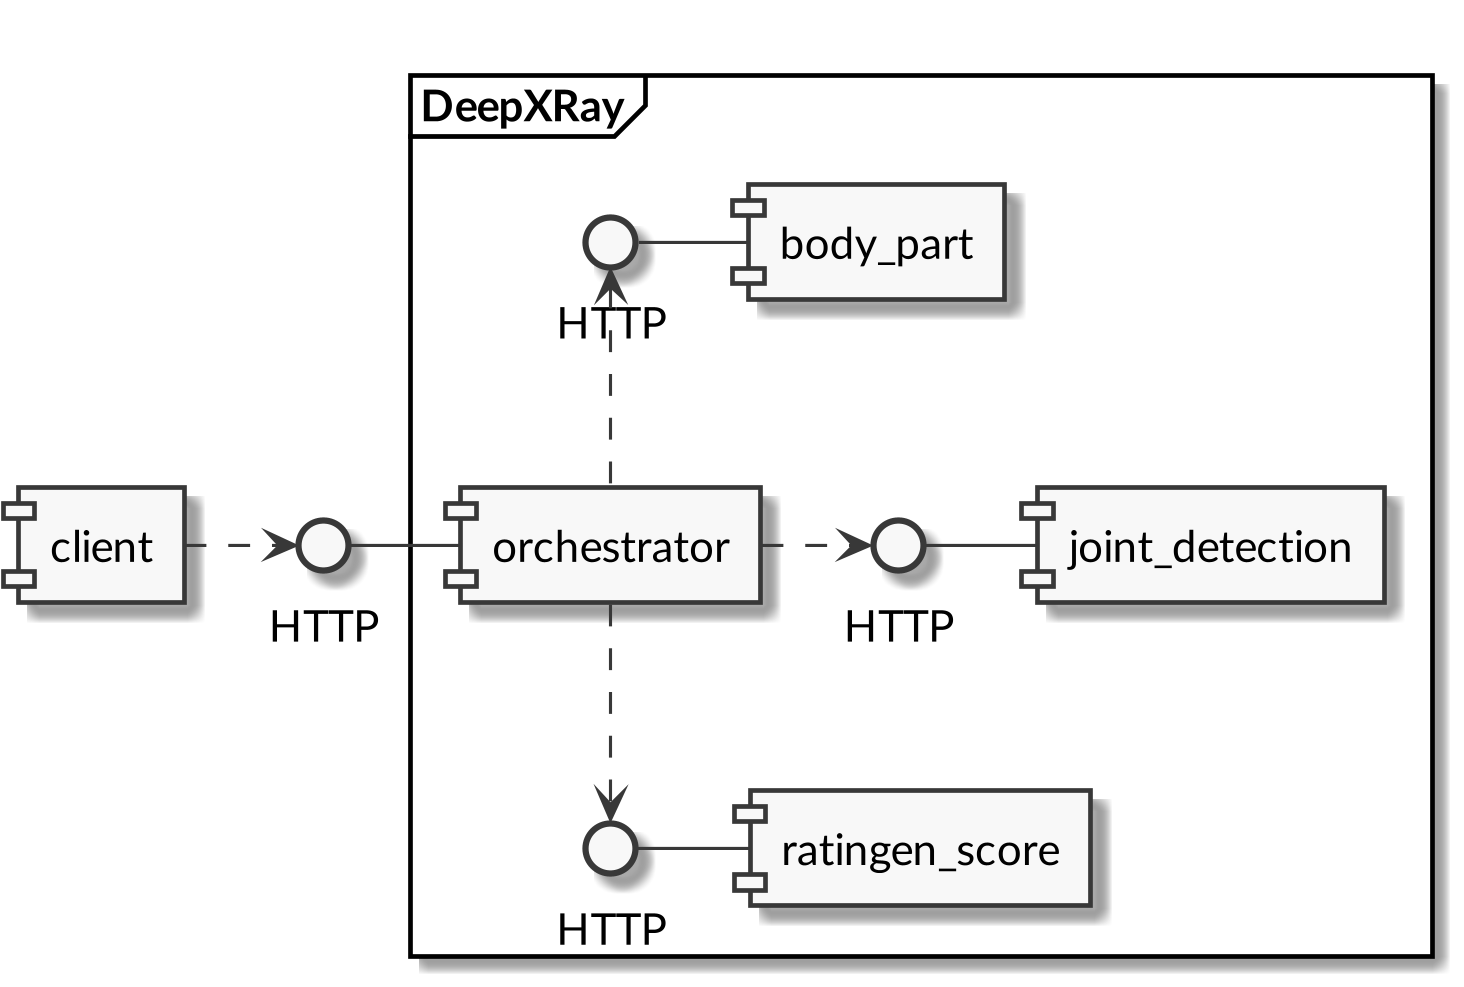
\includegraphics[width=\linewidth]{pics/architektur-variante-http.png}
    \caption{Komponentenarchitektur der Varianten 1 und 2 (HTTP, synchron und synchron/asynchron). Die Modellkomponenten bieten eine HTTP-Schnittstelle an, die vom \texttt{orchestrator} angesprochen wird. (Komponentendiagramm)}
    \label{fig:architektur-variante-http}
\end{figure}

Die Komponentenarchitektur dieser Variante ist auf \imgref{fig:architektur-variante-http} (Komponentendiagramm) ersichtlich. Die drei Modellkomponenten bieten jeweils eine interne HTTP-Schnittstelle an, die vom \texttt{orchestrator} angesprochen werden kann. Zwischen den Modellkomponenten findet keine Kommunikation statt.

\begin{figure}[tbh]
    \centering
    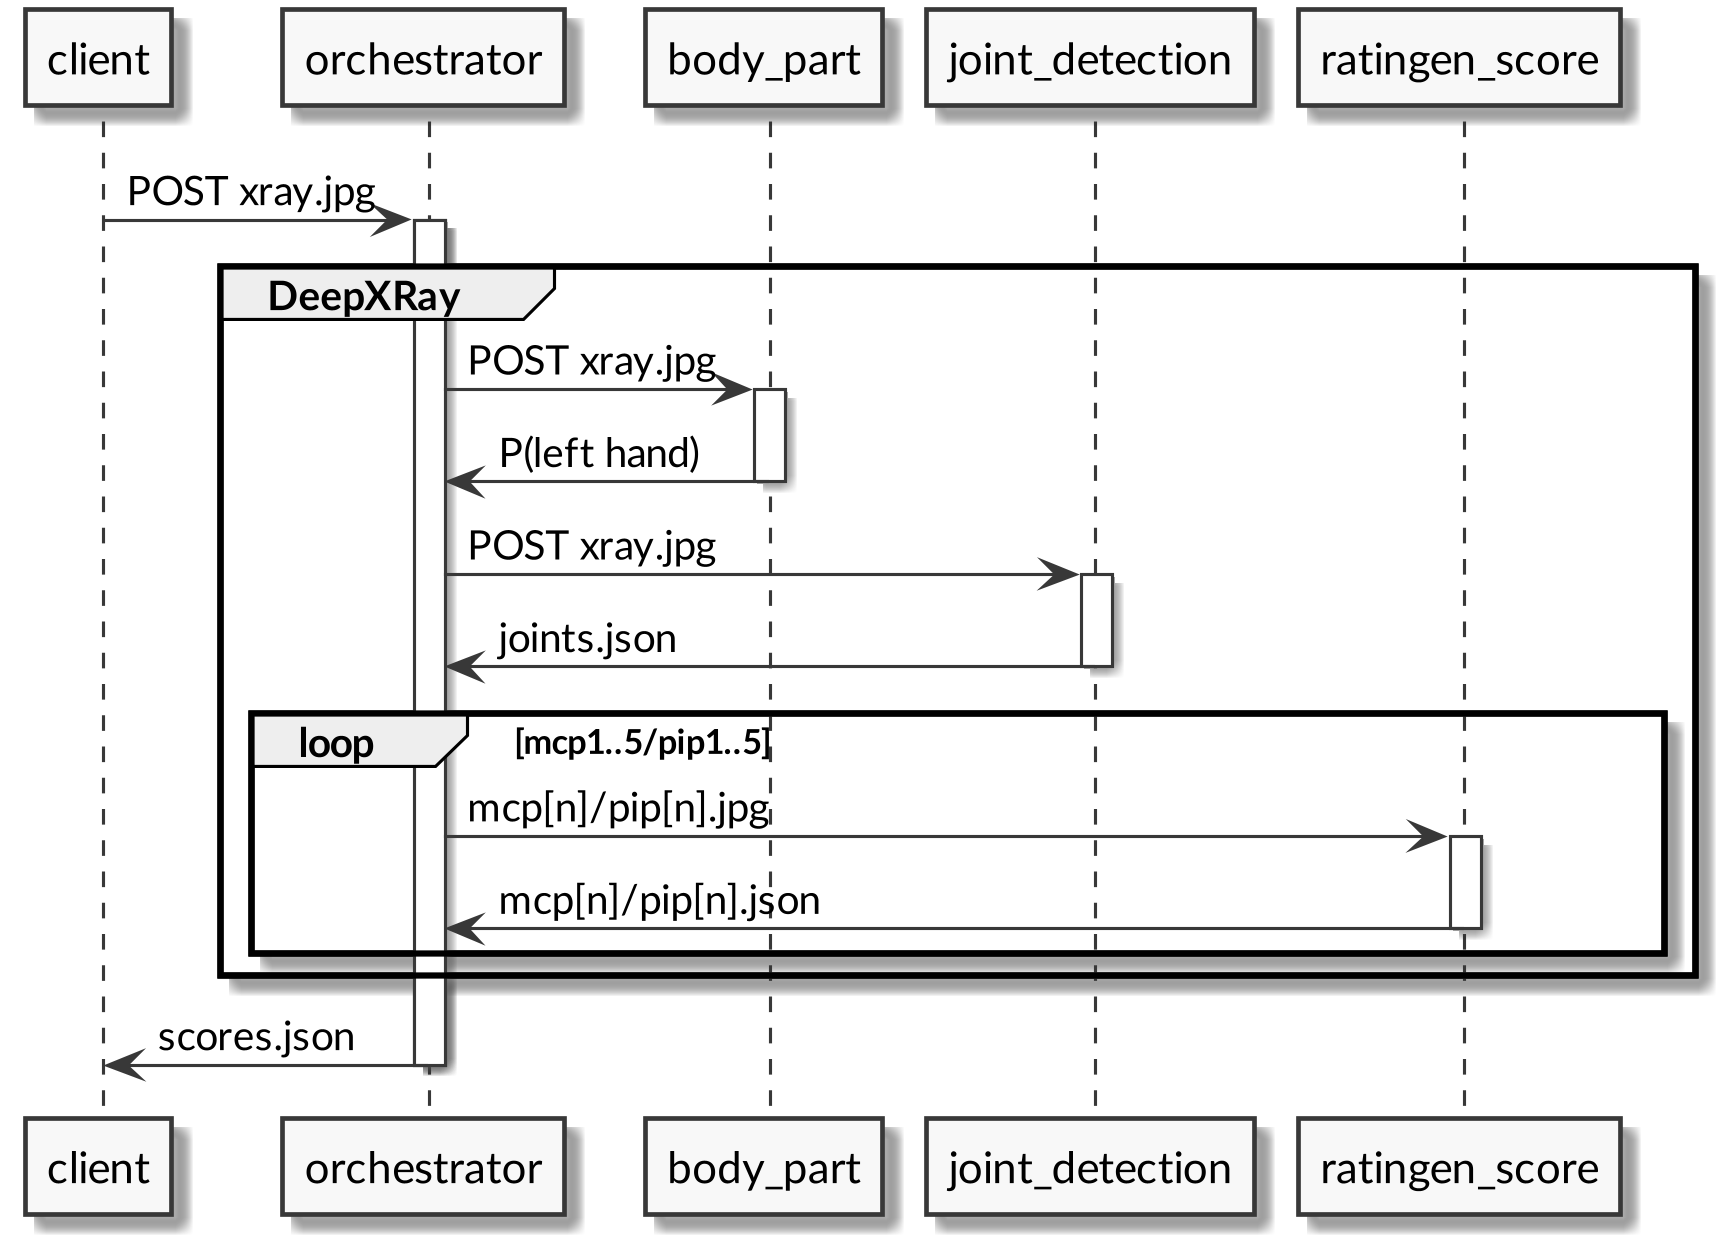
\includegraphics[width=\linewidth]{pics/datenfluss-variante-http-1.png}
    \caption{Datenfluss der Variante 1 (HTTP, synchron). Die einzelnen Modellkomponenten werden streng synchron aufgerufen und sequenziell abgearbeitet. (Sequenzdiagramm)}
    \label{fig:datenfluss-variante-http-1}
\end{figure}

Das Sequenzdiagramm \imgref{fig:datenfluss-variante-http-1} veranschaulicht den Ablauf. Zunächst stellt der \texttt{client} eine HTTP-\texttt{POST}-Anfrage an den \texttt{orchestrator}, welche ein Röntgenbild (\texttt{xray}) enthält. Der \texttt{orchestrator} leitet das Bild weiter zu \texttt{body\_part}. Diese Komponente antwortet mit einer Wahrscheinlichkeit, mit der es sich beim dargestellten Körperteil um eine linke Hand handelt.

Fällt diese Wahrscheinlichkeit genügend hoch aus, um eine Weiterverarbeitung zu rechtfertigen, wird das Röntgenbild weiter an die Komponente \texttt{joint\_detection} gesendet.\footnote{Auf Negativfälle wird in diesem Kapitel nur eingegangen, wo sie für die Konzeption der Architektur ausschlaggebend sind. Ansonsten wird zugunsten der Übersichtlichkeit auf deren Besprechung verzichtet. Negativfälle werden im Kapitel \secref{sec:realisierung} behandelt.} Dort werden die zehn relevanten Gelenke extrahiert und als Bildausschnitte in einem geeigneten Format\footnote{z.B. base64-codiert in einem JSON-Payload} an den \texttt{orchestrator} zurückgeliefert.

Der \texttt{orchestrator} sendet diese extrahierten Bildausschnitte der Reihe nach an die Komponente \texttt{ratingen\_score}, welche das Scoring der dargestellten Gelenke vornimmt. Die Score wird wiederum in einem geeigneten Format an den \texttt{orchestrator} zurückgesendet.

Am Schluss sammelt der \texttt{orchestrator} diese Scores, fasst sie in einer Datenstruktur zusammen, und sendet sie dem Client in einem geeigneten Format (JSON) zurück.

Diese Variante hat folgende Vor- und Nachteile:

\begin{description}
    \item[Vorteile] Die Variante ist sehr einfach umzusetzen. Da HTTP als externe Schnittstelle bereits gesetzt ist, können die internen Schnittstellen den gleichen Ansatz verwenden, wodurch nur eine Art von Schnittstelle benötigt wird.
    \item[Nachteile] Die Extraktion der Gelenke muss abgewartet werden, bis zum Scoring derselben übergegangen werden kann. Das Scoring findet streng sequenziell statt und ist daher langsam. Zu einem bestimmten Zeitpunkt kann jeweils nur eine Instanz der Modellkomponenten genutzt werden.
\end{description}

\subsubsection{Variante 2: HTTP, synchron und asynchron}

Die zweite Variante geht von der gleichen Komponentenarchitektur aus wie die erste Variante, siehe \imgref{fig:architektur-variante-http} (Komponentendiagramm). Im Gegensatz zur ersten Variante soll die zweite Variante jedoch nicht streng synchron arbeiten. Hierzu ändert sich die interne Arbeitsweise der \texttt{orchestrator}-Komponente und die Schnittstelle zur Komponente \texttt{joint\_detection}.

\begin{figure}[tbh]
    \centering
    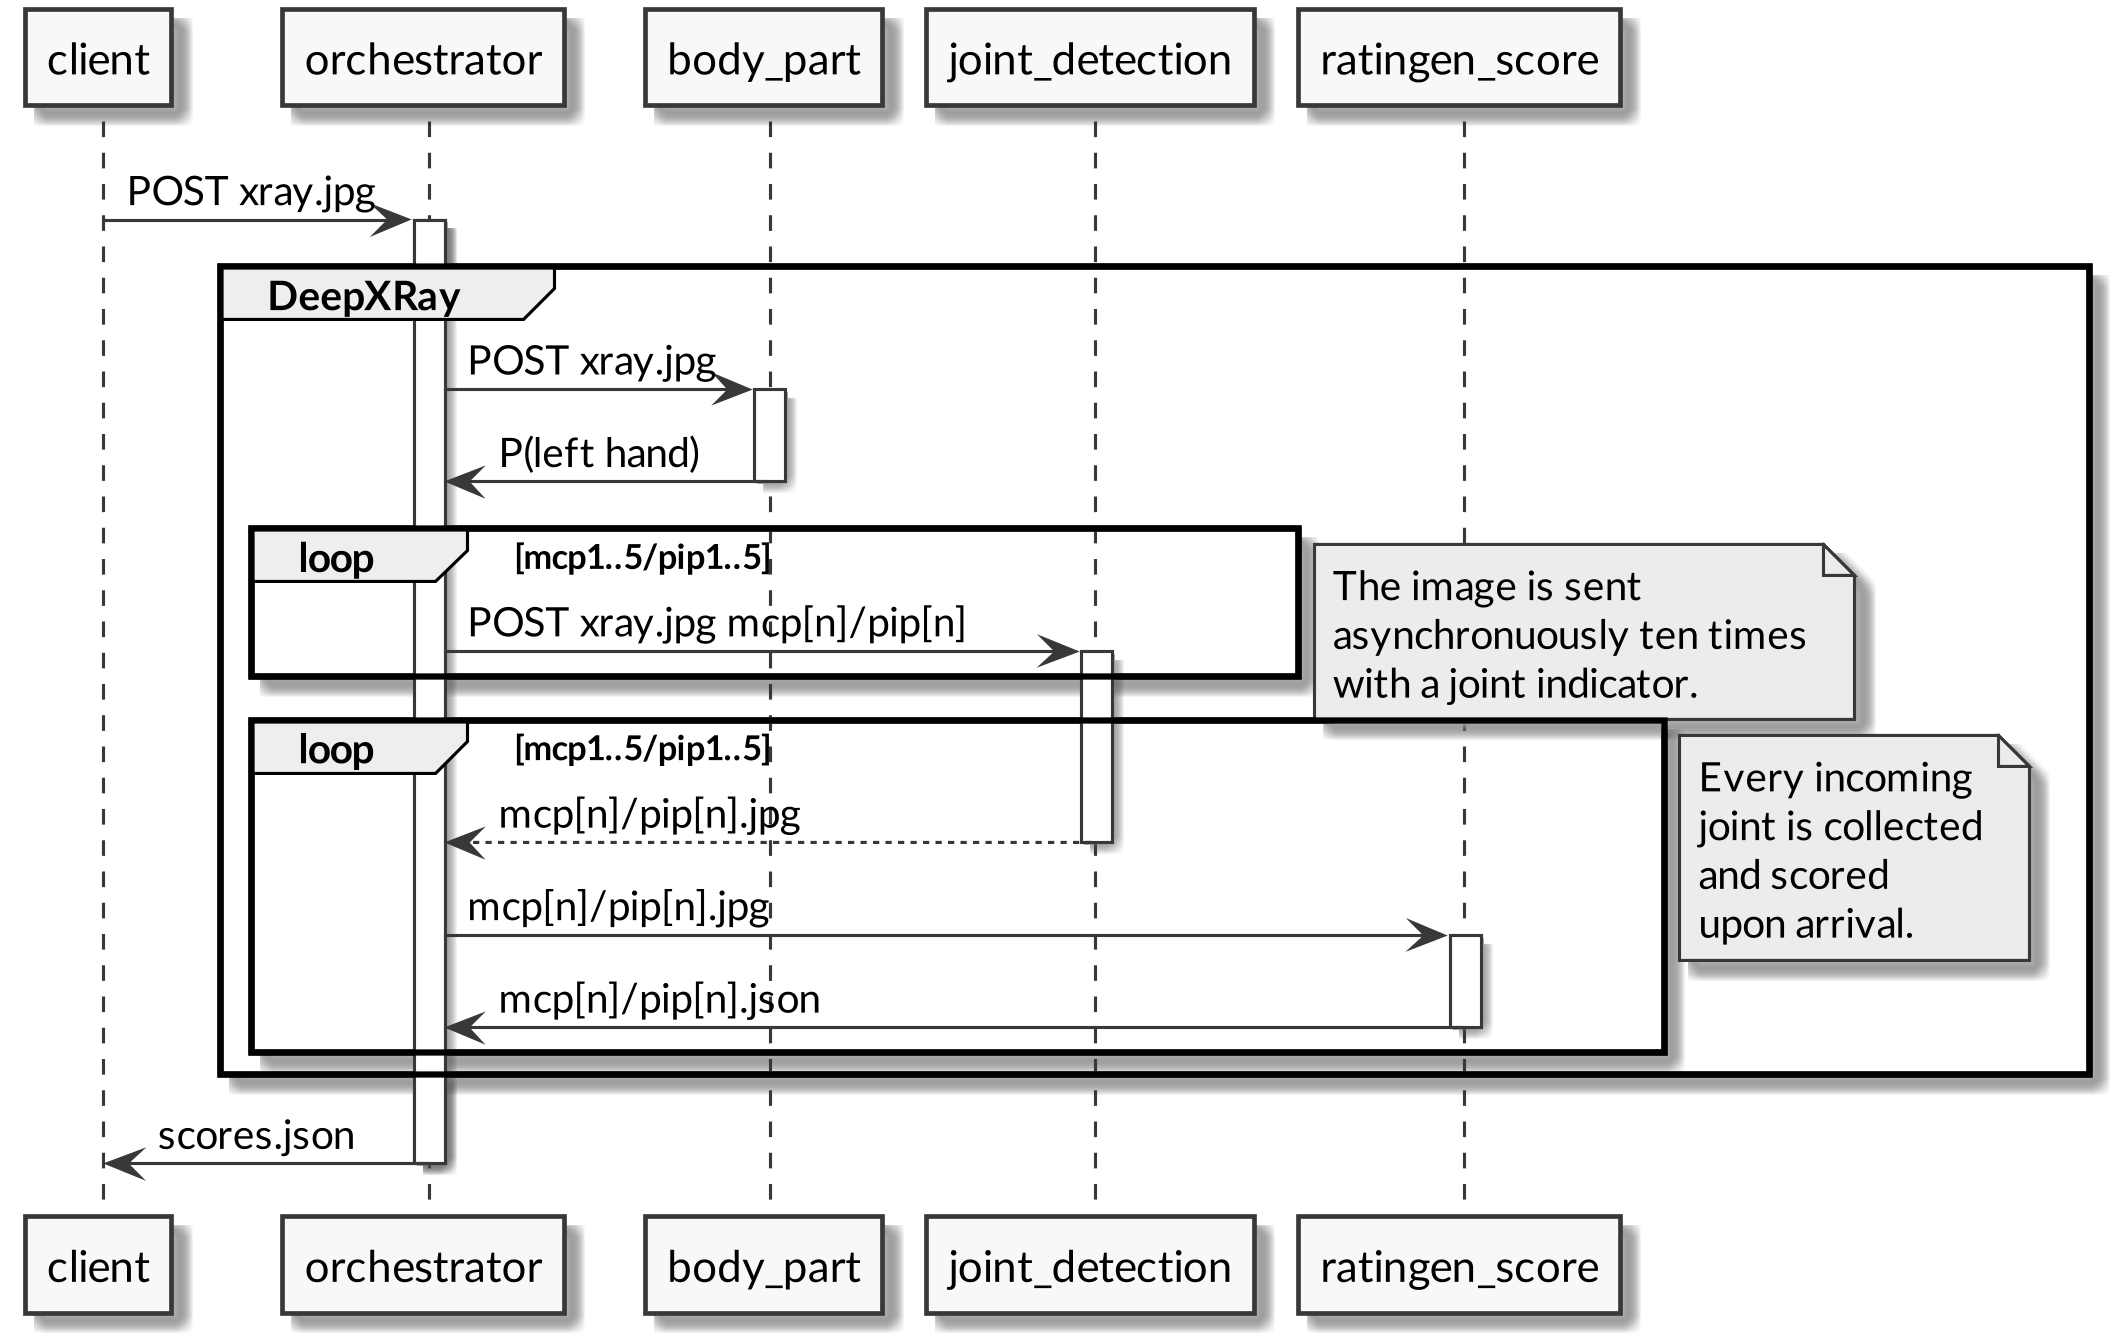
\includegraphics[width=\linewidth]{pics/datenfluss-variante-http-2.png}
    \caption{Datenfluss der Variante 2 (HTTP, synchron und asynchron). Es wird bereits mit dem Scoring begonnen, wenn das erste Gelenk extrahiert ist. (Sequenzdiagramm)}
    \label{fig:datenfluss-variante-http-2}
\end{figure}

Der geänderte Ablauf ist auf \imgref{fig:datenfluss-variante-http-2} ersichtlich. Die Erkennung des Körperteils auf dem Röntgenbild erfolgt wiederum über eine synchrone HTTP-\texttt{POST}-Anfrage an \texttt{body\_part}.

Die Extraktion der Gelenke bei der \texttt{joint\_detection}-Komponente erfolgt jedoch nicht mehr mit einer einzigen Anfrage, deren Antwort synchron abgewartet wird, sondern über eine Anfrage \textit{pro Gelenk}, d.h. es werden zehn Anfragen an \texttt{joint\_detection} gestellt: jeweils mit einem Röntgenbild und dem zu extrahierenden Gelenk. Diese Anfragen werden nebenläufig in einem Unterprozess pro Gelenk abgeschickt.

Sobald ein Unterprozess ein extrahiertes Gelenk von \texttt{joint\_detection} als Antwort erhält, kann damit eine Anfrage für das Scoring an die Komponente \texttt{ratingen\_score} gestellt werden, auf deren Antwort in jedem Unterprozess synchron gewartet wird.

Sind alle zehn Scores eingetroffen, können diese zu einer Antwort für den Client zusammengestellt und an diesen zurückgeschickt werden.

Diese hybride Variante (HTTP asynchron/synchron gemischt) hat Vorteile gegenüber der streng synchronen Variante, löst aber nicht alle Probleme:

\begin{description}
    \item[Vorteile] Es kann bereits mit dem Scoring der Gelenke begonnen werden, wenn das erste Gelenk extrahiert worden ist. So können \texttt{joint\_detection} und \texttt{ratingen\_score} gleichzeitig arbeiten, wodurch die Anfrage des Clients schneller bedient werden kann.
    \item[Nachteile] Das Röntgenbild wird zehnmal statt nur einmal an \texttt{joint\_detection} geschickt. Die Koordination nebenläufiger HTTP-Anfragen ist anspruchsvoller. Ohne zusätzlichen Load-Balancer ist weiterhin nur eine Instanz pro Komponente einsetzbar.
\end{description}

\subsubsection{Variante 3: Messaging zwischen Modellkomponenten}
\label{sec:variante-3-messaging}

Soll die Verarbeitung von Röntgenbildern mit mehreren Instanzen pro Komponente, d.h. parallel vonstatten gehen, wäre mit HTTP ein Load-Balancer pro Komponente nötig. Eine Alternative hierzu stellt das Messaging dar, welches in Abschnitt \secref{sec:integrationsvarianten} vorgestellt worden ist.

Dabei wird die Arbeit nicht an die einzelnen Komponenten erteilt wie bei HTTP (Push), sondern von den einzelnen Komponenten (bzw. deren Instanzen) von einer Queue selbständig abgeholt (Pull). Dies ermöglicht eine parallele Abarbeitung, indem sich die unbeschäftigen Instanzen einer Komponente jeweils neue Arbeit nach dem Round-Robin-Verfahren von der Queue abholen.

\imgref{fig:architektur-variante-queue-1} zeigt eine mögliche Komponentenarchitektur, bei der intern nicht HTTP, sondern Messaging zum Einsatz kommt.\footnote{Hier fällt auf, dass die einzelnen Komponenten jeweils eine Queue \textit{verwenden}, diese aber von keiner der involvierten Komponenten zur Verfügung gestellt wird. Tatsächlich werden die Queues in der Regel von einem \textit{Message-Broker} zur Verfügung gestellt, der aus Gründen der Übersichtlichkeit nicht dargestellt ist. Andererseits gibt es auch Messaging-Lösungen, die ohne Message-Broker-Komponente auskommen, z.B. ZeroMQ.} Bei dieser Variante werden die Komponenten der Reihe nach jeweils paarweise mit einer Queue verbunden, wodurch ein geschlossener Kreis entsteht. Über eine Error-Queue kann der Ablauf im Fehlerfall abgebrochen und als entsprechende Fehlermeldung an den \texttt{orchestrator} weitergegeben werden.

\begin{figure}[tbh]
    \centering
    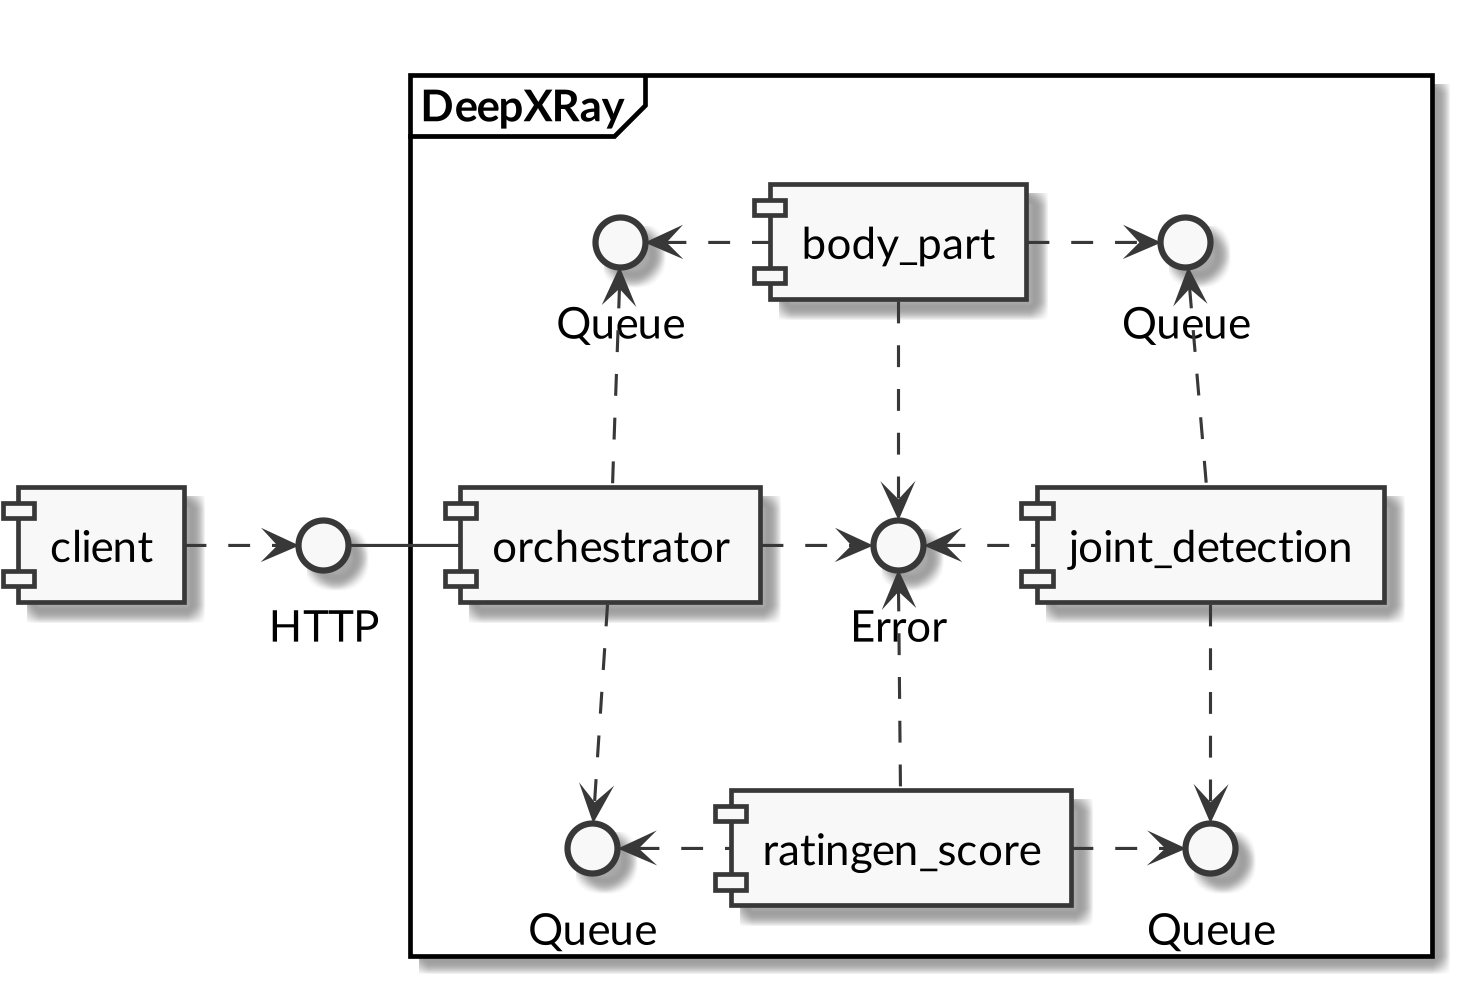
\includegraphics[width=\linewidth]{pics/architektur-variante-queue-1.png}
    \caption{Komponentenarchitektur der Variante 3 (Messaging zwischen den Modellkomponenten). Mithilfe von Message-Queues werden die Komponenten paarweise miteinander verbunden, und bilden so einen Kreis.}
    \label{fig:architektur-variante-queue-1}
\end{figure}

Gegenüber den ersten beiden Varianten (HTTP rein synchron und hybrid, d.h. asynchron/synchron) ändert sich der Ablauf grundlegend (siehe \imgref{fig:datenfluss-variante-queue-1}). Der \texttt{orchestrator} empfängt wiederum das Röntgenbild per HTTP vom Client. Er reicht dieses über eine Queue weiter an die Komponente \texttt{body\_part}. Hier gibt der \texttt{orchestrator} die Kontrolle über die Weiterverarbeitung ab.

Wird auf dem Röntgenbild eine linke Hand erkannt, reicht \texttt{body\_part} das Röntgenbild zur Extraktion der Gelenke an \texttt{joint\_detection} weiter, wiederum über eine Queue. Hier werden die zehn Gelenke der Reihe nach extrahiert. Jedes extrahierte Gelenk wird sogleich über eine weitere Queue an \texttt{ratingen\_score} weitergegeben. Es kann wiederum mit dem Scoring begonnen werden, wenn die Extraktion der Gelenke noch in Gang ist.

Die Scores werden von \texttt{ratingen\_score} über eine Queue an den \texttt{orchestrator} weitergereicht. Treten bei der Extraktion oder beim Scoring Fehler auf, werden diese über eine Error-Queue an den \texttt{orchestrator} gemeldet. Dieser braucht pro ursprünglich eingegangenem Request (Röntgenbild) zwei Queues zu beobachten: Die ermittelten Scores und die gemeldeten Fehler. Insgesamt müssen pro Vorgang zehn Nachrichten beim \texttt{orchestrator} eingehen, seien dies Scores oder Fehlermeldungen. Sind diese alle eingetroffen, kann der Client bedient werden.

\begin{figure}[tbh]
    \centering
    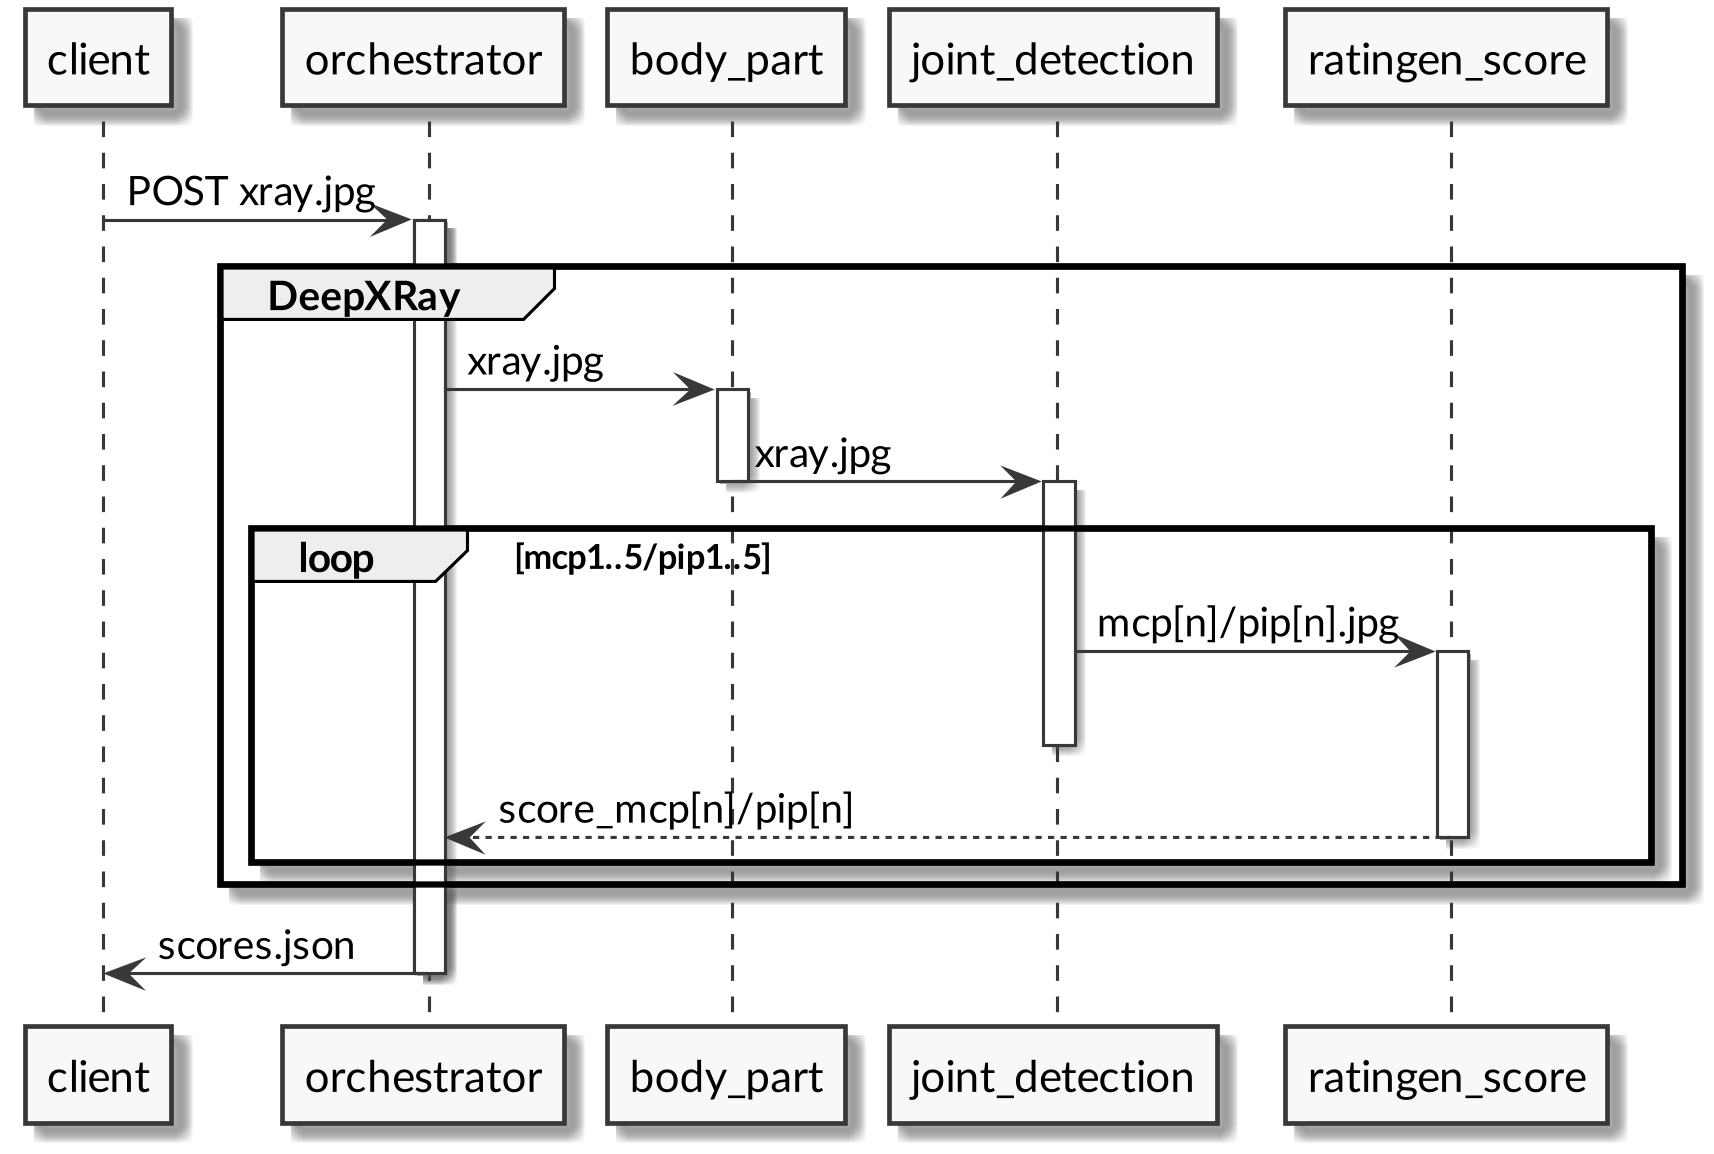
\includegraphics[width=\linewidth]{pics/datenfluss-variante-queue-1.png}
    \caption{Datenfluss der Variante 3 (Messaging zwischen den Modellkomponenten). Die Anfragen werden via Message-Queue von Komponente zu Komponente weitergereit. (Sequenzdiagramm)}
    \label{fig:datenfluss-variante-queue-1}
\end{figure}

Die asynchrone Verarbeitung über Message-Queues ermöglicht es, dass alle drei Modellkomponenten mit beliebig vielen Instanzen ausgeführt werden können, was die Verarbeitungsgeschwindigkeit bis zu einem gewissen Grad erhöht. Das «Einsammeln» der Ergebnisse wird über diese asynchrone Abarbeitung jedoch erschwert, zumal zu einem bestimmten Zeitpunkt die Nachrichten verschiedener Anfragen in den Queues hängen können. Der \texttt{orchestrator} benötigt darum einen Mechanismus, um die  eintreffenden Nachrichten einer ursprünglichen HTTP-Anfrage zuordnen zu können. Andernfalls könnte der Client mit seiner Antwort Informationen bekommen, die zu anderen Anfragen gehören.

Dieses Problem kann mit einem \textit{Correlation Identifier} gelöst werden \cite[S. 163-169]{enterprise-integration-patterns}. Hierzu wird jeder Anfrage eine eindeutige Identifikation zugewiesen. Dies kann eine fortlaufende Nummerierung sein, oder aber ein generierter Zufallswert. Wichtig ist, dass dieser Wert im gegebenen Kontext eindeutig ist. Die Message wird mit diesem Correlation Identifier ausgestattet und für Folgenachrichten übernommen. Sammelt der \texttt{orchestrator} die eingehenden Nachrichten von den beiden Queues ein, kann er diese über den Correlation Identifier dur urpsprünglichen Anfrage zuordnen.

Diese auf Messaging basierte Architekturvariante stellt in vielerlei Hinsicht eine Verbesserung gegenüber den beiden HTTP-Varianten dar, bringt aber auch neue Probleme mit sich:

\begin{description}
    \item[Vorteile] Über den Messaging-Ansatz wird eine parallele Abarbeitung ohne zusätzliche Load-Balancer ermöglicht.
    \item[Nachteile] Das asynchrone «Einsammeln» von Nachrichten und deren Zuordnung zu den ursprünglichen Client-Anfragen erfordert einen zusätzlichen Mechanismus (Correlation Identifier). Die dezentrale Kommunikation zwischen den Modellkomponenten ist komplizierter, da es mehr Kommunikationspaare gibt.
\end{description}

Zudem funktioniert der beschriebene Ansatz nur für das unmittelbar gegebene Problem: das Scoring von (linken) Händen, wobei immer genau zehn Gelenke von Interesse sind. Sollen in Zukunft auch die Röntgenbilder anderer Körperteile verarbeitet werden, etwa Becken mit zwei Hüftgelenken, funktioniert dieser Ansatz nicht mehr. Das Problem ist, dass der \texttt{orchestrator} nicht erfährt, welches Körperteil auf einem Röntgenbild dargestellt wird, und so nicht wissen kann, wie viele Scores (oder Fehlermeldungen) er einzusammeln hat.

\subsubsection{Variante 4: Messaging, synchron und asynchon}
\label{sec:variante-4-messaging}

Um für zukünftige Erweiterungen von anderen Körperteilen gerüstet zu sein, muss der \texttt{orchestrator} wissen, welches Körperteil auf einem Röntgenbild dargestellt ist, um so die richtige Anzahl an Scores bzw. Fehlermeldungen erwarten zu können. Darum wird \texttt{body\_part} gegenüber der Variante 3 aus dem Kreis der vier Komponenten entfernt und synchron an den \texttt{orchestrator} gekoppelt. Die Komponentenarchitektur ist auf \imgref{fig:architektur-variante-queue-2} ersichtlich.

\begin{figure}[tbh]
    \centering
    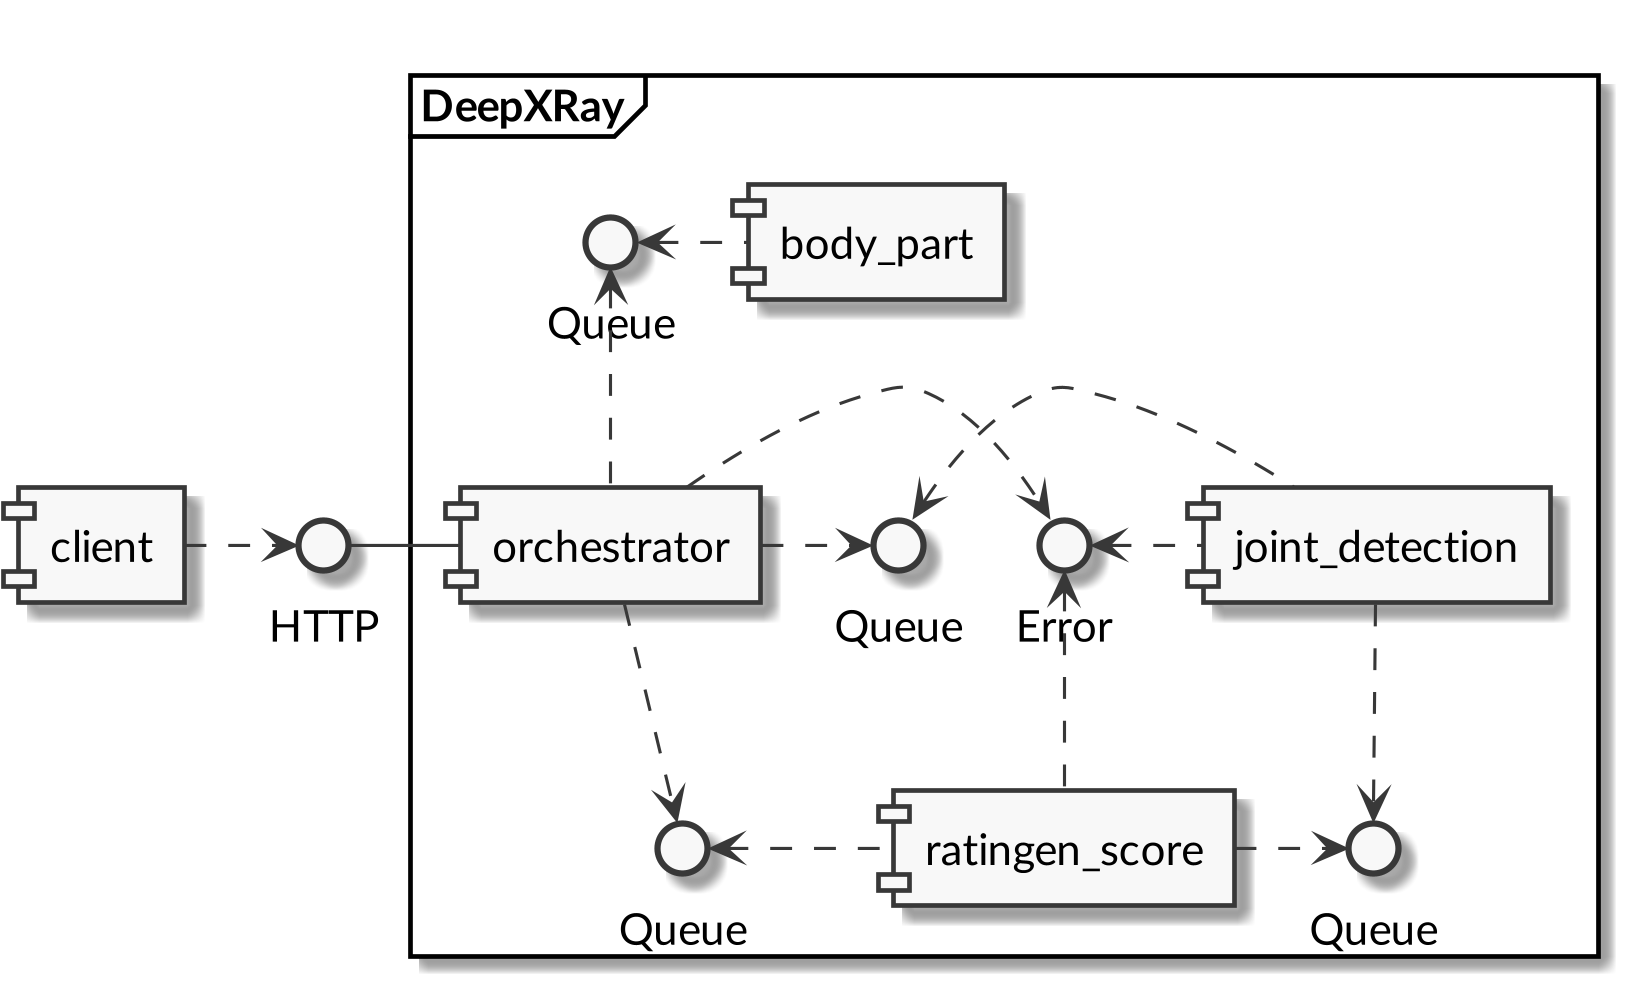
\includegraphics[width=\linewidth]{pics/architektur-variante-queue-2.png}
    \caption{Komponentenarchitektur der Variante 4 (Messaging, synchron und asynchron). Die \texttt{body\_part}-Komponente ist synchron, die anderen Modellkomponenten sind asynchron angebunden.}
    \label{fig:architektur-variante-queue-2}
\end{figure}

Obwohl die Kommunikation zwischen \texttt{body\_part} und dem \texttt{orchestrator} synchron abläuft, soll dennoch eine Message-Queue als Schnittstelle zwischen diesen Komponenten dienen. Dies hat den Vorteil, dass \texttt{body\_part} mit mehreren Instanzen gleichzeitig betrieben werden kann, die sich die Workloads abwechselnd von der Queue holen, die nicht nur als Übertragungsmedium, sondern auch als Load-Balancer fungiert.

Der Datenfluss ändert sich dabei gegenüber der vorherigen Messaging-Variante beträchtlich (siehe \imgref{fig:datenfluss-variante-queue-2}). Das Körperteil wird ‒ wie bei den beiden HTTP-Varianten ‒ synchron detektiert. Wurde eine linke Hand erkannt, gibt der \texttt{orchestrator} ‒ und nicht \texttt{body\_part}! ‒ die Extraktionen in Auftrag. Da hier nun Messaging zum Einsatz kommt, können zehn entsprechende Nachrichten auf der Queue publiziert werden, von der \texttt{joint\_detection} liest.

Extrahierte Gelenke werden über eine weitere Queue an \texttt{ratingen\_score} weitergeleitet. Scheitert die Extraktion oder das Scoring, kann dies über eine Error-Queue an den \texttt{orchestrator} gemeldet werden. Da dieser die Extraktion der Gelenke in Auftrag gegeben hat, ist diesem die Anzahl der zu erwartenden Nachrichten bekannt. Sind diese Nachrichten eingetroffen, kann er den Client damit bedienen.

\begin{figure}[tbh]
    \centering
    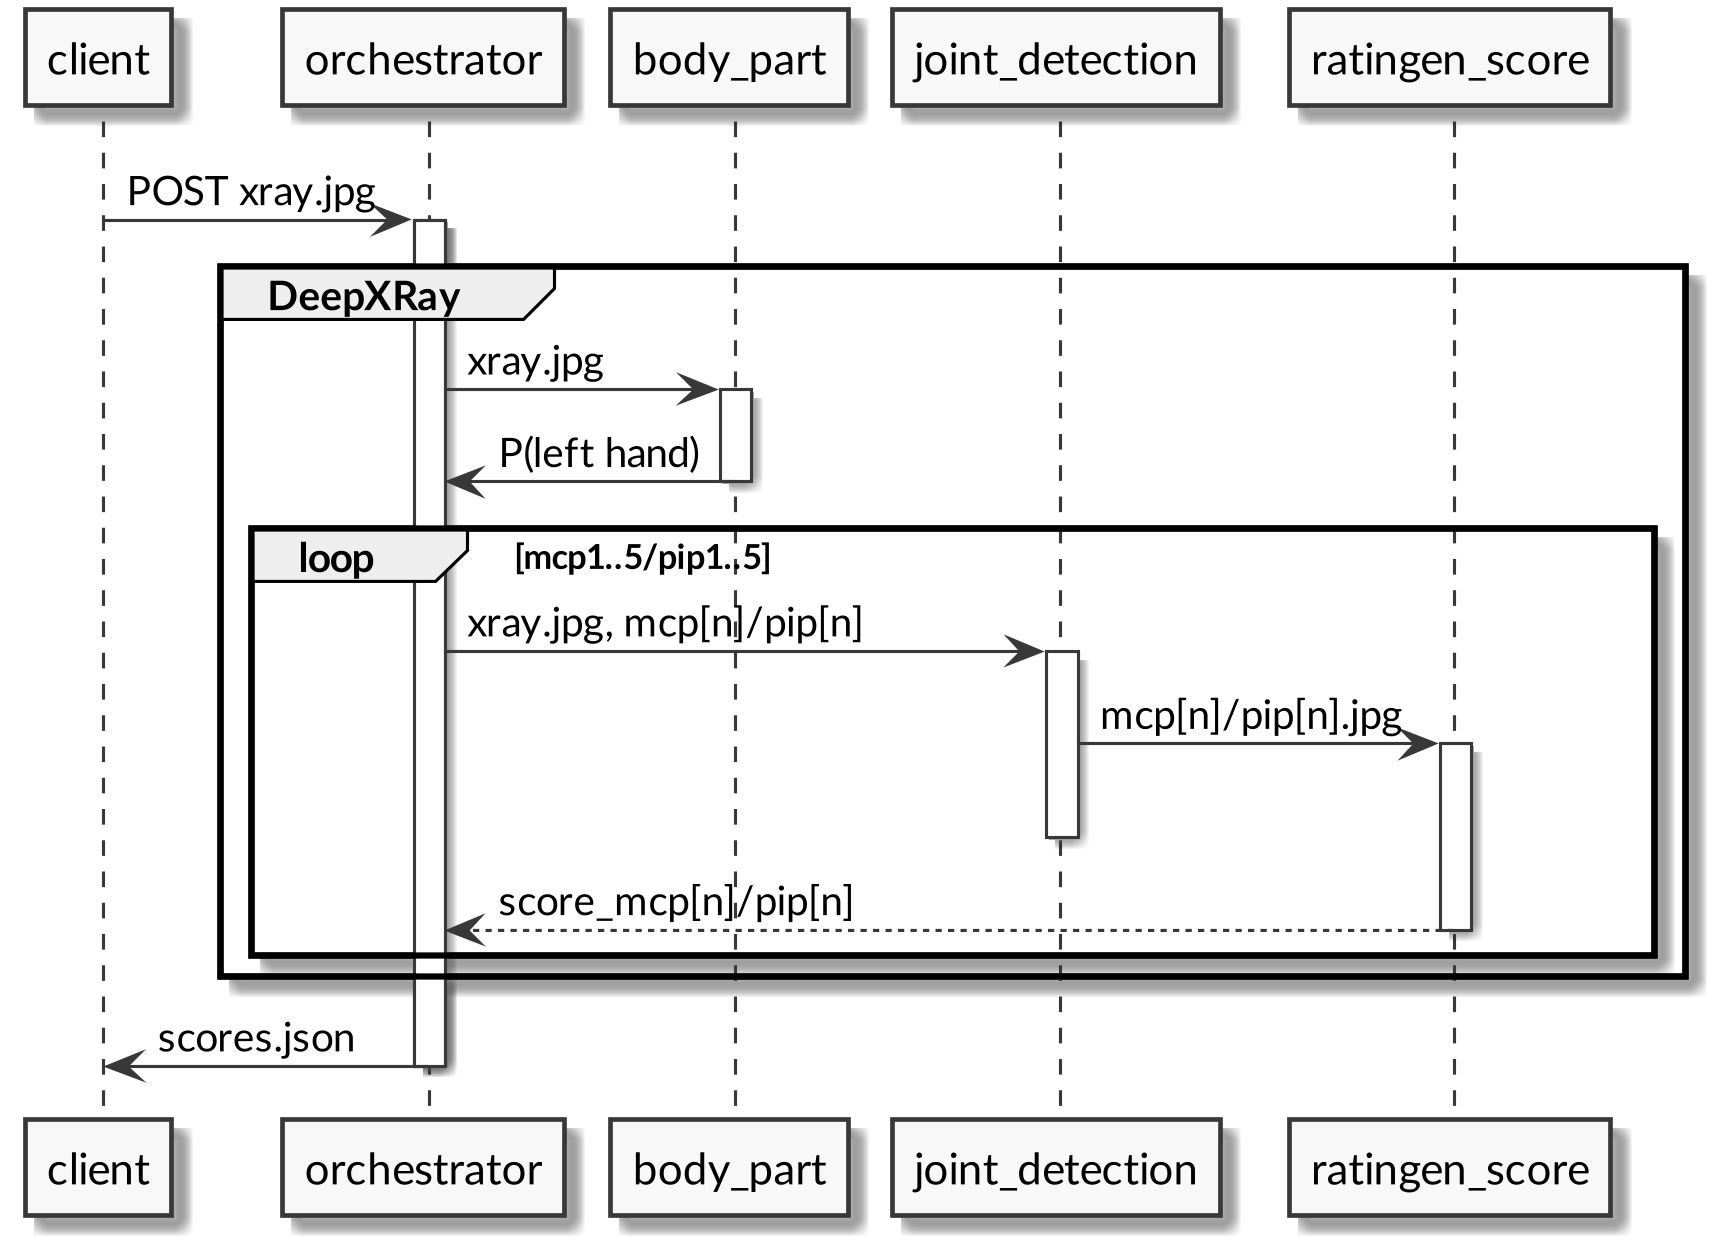
\includegraphics[width=\linewidth]{pics/datenfluss-variante-queue-2.png}
    \caption{Datenfluss der Variane 4 (Messaging, synchron und asynchron). Die Modellkomponente \texttt{body\_part} wird synchron, die Modellkomponenten \texttt{joint\_detection} und \texttt{ratingen\_score} werden asynchron angebunden. (Sequenzdiagramm)}
    \label{fig:datenfluss-variante-queue-2}
\end{figure}

Diese Variante kombiniert die Vorteile der synchronen Erkennung des Körperteils mit den Vorteilen der nebenläufigen Extraktion und dem Scoring der Gelenke:

\begin{description}
    \item[Vorteile] Die Gelenke können nebenläufig extrahiert und gescored werden, was eine höhere Verarbeitungsgeschwindigkeit ermöglicht. Mithilfe von Messaging können die Komponenten mit mehreren Instanzen parallel betrieben werden. Zudem funktioniert die Architektur auch dann noch, wenn andere Körperteile als linke Hände (mit einer anderen Anzahl relevanter Gelenke) verarbeitet werden sollen.
    \item[Nachteile] Das «Einsammeln» der Nachrichten erfordert ‒ gleich wie die vorherige Mes\-sag\-ing-Variante ‒ einen Correlation Identifier. Der \texttt{orchestrator} hat noch mehr Kommunikationsaufgaben. Zudem wird das Röntgenbild einmal pro Gelenk publiziert, nicht einmal für alle zehn Gelenke.
\end{description}

\subsubsection{Entscheidung}

Jede Variante bietet Vorteile gegenüber ihrem Vorgänger: Variante 1 (HTTP, synchron) arbeitet streng sequenziell. Variante 2 (HTTP, asynchron/synchron) kann bereits mit dem Scoring beginnen, wenn die Extraktion noch nicht abgeschlossen ist. Variante 3 (Mes\-sag\-ing zwischen Modellkomponenten) ermöglicht die Ausführung mehrerer Instanzen eines Modells. Variante 4 (Messaging, synchron und asynchron) lässt sich darüber hinaus am besten erweitern. Trotz der Nachteile von Variante 4 ‒ Notwendigkeit eines Correlation Identifiers, mehrfache Publikation des Röntgenbilds (einmal pro Gelenk), verschiedenartige Kommunikationsaufgaben (synchron und asynchron) ‒ ist sie die flexibelste und am besten erweiterbare Variante.

Der Prototyp soll darum gemäss Variante 4 (Messaging, synchron und asynchron) umgesetzt werden.

\subsection{Austauschbarkeit von Modellen}
\label{sec:austauschbarkeit-von-modellen}

Die Modelle ‒ oder Modellkomponenten ‒ müssen gemäss Projektauftrag (siehe \secref{sec:erwartetes-resultat}) austauschbar sein. Für diese Anforderung gibt es verschiedene Lösungsansätze.

Ein Lösungsansatz wäre die Austauschbarkeit auf Modellebene. Hierzu wurden entsprechende Formate ‒ TensorFlow SavedModel und ONNX ‒ im Abschnitt \secref{sec:modellformate} vorgestellt. Die bestehenden Modelle lassen sich jedoch nicht einfach in eines dieser Formate konvertieren. Zudem ist die Wahl eines dieser Formate noch keine Garantie für Vorwärtskompatibilität in einigen Jahren. Ändert sich die Modellspezifikation (Inputs, Outputs) nur geringfügig, ist die Austauschbarkeit auf Modellebene bereits nicht mehr gegeben. Die Austauschbarkeit von Modellen (oder Modellkomponenten) über die Modelldatei ist somit für das vorliegende Projekt keine Option.

Statt die Modelle selber austauschbar zu machen, und so Änderungen an ihren Inputs und Outputs für längere Zeit zu verunmöglichen, können die Modell\textit{komponenten} austauschbar gemacht werden. Hierfür wird eine API spezifiziert, an die sich die Modellkomponenten halten müssen. Da für den Prototyp Messaging zum Einsatz kommen soll (siehe \secref{sec:variante-4-messaging}), ist diese API einerseits über das Nachrichtenformat, andererseits über die verwendete Messaging-Technologie (z.B. AMQP oder MQTT) zu definieren.

Da die verwendeten Modelle auf verschiedenen Versionen von TensorFlow basieren und mit unterschiedlichen High-Level-APIs (tflearn, Keras) erstellt worden sind, können diese nicht in der gleichen Laufzeitumgebung ausgeführt werden.

Mit virtuellen Python-Umgebungen ist es möglich, auf dem gleichen Rechner verschiedene Python-Versionen mit den dazugehörigen Libraries und Frameworks auszuführen. Mit dem Modul \texttt{venv} \footnote{\url{https://docs.python.org/3/library/venv.html} (abgerufen am 11.05.2020)} können verschiedene virtuelle Python-Um\-ge\-bung\-en auf einem Rechner erstellt werden, die auf der installierten Python-Version basieren.

Da die verwendeten Frameworks/Libraries jedoch nicht zu den neuesten Versionen von Python kompatibel sind, müssten auch verschiedene Versionen des Python-In\-ter\-pret\-ers installiert werden können. Das Modul \texttt{pyenv}\footnote{\url{https://github.com/pyenv/pyenv} (abgerufen am 11.05.2020)} unterstützt dies. Diese Variante ist aber für den Produktiveinsatz riskant, zumal mehrere ältere Versionen des Python-Interpreters auf dem gleichen System laufen, und so den Angriffsvektor dieses Systems vergrössern.\footnote{Das gestellte Problem ist ja, dass aufgrund von Inkompatibilitäten auf Ebene Libraries/Frameworks ältere Versionen von Python verwendet werden müssen. Das Modell \texttt{ratingen\_score} wurde etwa mit Python 3.5 erstellt ‒ eine Version, die nur noch bis am 13.09.2020 Updates erhalten soll (\url{https://devguide.python.org/\#branchstatus}, abgerufen am 11.05.2020).}

Container ermöglichen nicht nur die Installation praktisch beliebiger (älterer) Versionen von Python, sondern auch die Isolation dieser Umgebungen. So können ältere Versionen verwendet werden, ohne die Sicherheit des zugrundeliegenden Systems zu beeinträchtigen. Container-Runtimes wie Docker ermöglichen es zudem, Ports für die Kommunikation zwischen dem Container und dem zugrundeliegenden System bzw. Ports zwischen einzelnen Containern per Konfiguration zu definieren.

Werden die Modellkomponenten als Container umgesetzt, können sie auf Basis ihrer Schnittstelle ‒ Messaging-Format, Messaging-Protokoll und Port ‒ austauschbar gemacht werden. Welche Libraries, Frameworks, Python-Versionen und Modellformate dabei zum Einsatz kommen, ist für die Umsysteme nicht relevant.

Die Austauschbarkeit von Modellkomponenten soll darum mithilfe von Containern gewährleistet werden.

\subsection{Parallelisierung ‒ Nebenläufigkeit}

Der Projektauftrag nennt das «Verteilen über mehrere GPUs» als Anforderung (siehe \secref{sec:erwartetes-resultat}). Dieser ist nicht ohne Weiteres nachzukommen, da zur Ausführung eines Modells auf einer GPU dieses komplett in den Speicher derselben geladen werden muss. Da für die Gelenkextraktion nicht nur ein Modell, sondern zehn verschiedene Modelle in den Speicher geladen werden müssen, dürfte eine Vielzahl von GPUs nötig sein, um die Ausführung damit zu beschleunigen. Ein solches Setup steht für die Entwicklung nicht und für den Produktiveinsatz wohl kaum zur Verfügung.\footnote{Der Cloud-Anbieter Exoscale, der auch Hosting in der Schweiz anbietet, was für sensible Patientendaten wie Röntgenbilder auch erforderlich ist, verlangt für eine Instanz mit vier GPUs 2.28 € pro Stunde, d.h. bis zu 1696.32 € pro Monat.}

Auch wenn dieses optimale, auf GPUs basierende Setup vorerst keine Option ist, ist die parallele Ausführung der verschiedenen Modelle für eine akzeptable End-to-End-Perfomance unbedingt erforderlich ‒ und darum auch für die Architekturdiskussion (siehe \secref{sec:architekturvarianten}) eine grundlegende Anforderung.

Doch genügt eine geeignete Architektur, um Parallelisierung zu gewährleisten? Um diese Frage beantworten zu können, lohnt sich ein genauerer Blick auf die Begriffe \textit{Nebenläufigkeit} (engl. \textit{concurrency}) und \textit{Parallelität} (engl. \textit{parallelism}).

Die Begriffe werden oft synonym gebraucht, haben aber unterschiedliche Bedeutungen ‒ die zugegebenermassen in einer Welt mit allgegenwärtigen Multicore-Systemen kaum noch erfahrbar sind.

Doch der Reihe nach: Rob Pike, einer der Schöpfer der Programmiersprache Go, definiert die beiden Begriffe folgendermassen: \textit{«Concurrency and Parallelism are not the same thing. \[...\] Concurrency is \[...\] the composition of independently executing processes. Parallelism, on the other hand, ist the simultaneous execution of multiple things. \[...\] One is really about structure (concurrency), and one is about execution (parallelism).»}\footnote{Nebenläufigkeit und Parallelität sind nicht das Gleiche. Nebenläufigkeit ist die Komposition unabhängig voneinander ablaufender Prozesse. Parallelität hingegen ist die gleichzeitige Ausführung mehrerer Dinge. Bei einem geht es um die Struktur (Nebenläufigkeit), beim anderen geht es um die Ausführung (Parallelität). (Übersetzung des Autors)} \cite[ab 1:16]{concurrency-is-not-parallelism}.

Joe Armstrong, der 2019 verstorbene Schöpfer der Programmiersprache Erlang, geht genauer auf die Hardware-Aspekte dieser Konzepte ein: \textit{«In everyday language, words like concurrent, simultaneous, and parallel mean almost the same thing. But in programming languages, we need to be more precise. In particular, we need to distinguish between concurrent and parallel programs. If we have only a single-core computer, then we can never run a parallel program on it. This is because we have one CPU, and it can do only one thing at a time. We can, however, run concurrent programs on a single-core computer. The computer time-shares between the different tasks, maintaining the illusion that the different tasks run in parallel.»}\footnote{In der Alltagssprache bedeuten Wörter wie «nebenläufig», «gleichzeitig» und «parallel» fast das Gleiche. Bei Programmiersprachen muss man aber präziser sein. Besonders «nebenläufig» und «parallel» muss man voneinander unterscheiden. Hat man nur einen Single-Core-Computer, kann man niemals ein paralleles Programm auf ihm laufen lassen. Das liegt daran, dass man nur eine CPU hat, und diese kann nur eine Sache zur gleichen Zeit machen. Wir können jedoch ein nebenläufiges Programm auf einem Single-Core-Computer ausführen. Der Computer wechselt zwischen den verschiedenen Aufgaben hin und her, und hält die Illusion aufrecht, mehrere Aufgaben parallel abzuarbeiten. (Übersetzung des Autors)} \cite[S. 8]{programming-erlang}.

Parallelisierung erreicht man also dadurch, indem man ein nebenläufiges Programm auf Hardware mit mehreren CPU-Kernen bzw. mehreren CPUs laufen lässt. Ein nebenläufiges Programm muss so strukturiert sein, dass es potenziell mit mehreren Vorgängen gleichzeitig zurecht kommt. Eine solche Struktur wurde in der Architekturdiskussion erarbeitet (siehe \secref{sec:variante-4-messaging}). Wird der Prototyp entsprechend umgesetzt, ist Parallelität praktisch automatisch gegeben, zumal heute kaum noch Rechner mit nur einem CPU-Kern im Einsatz sind.

\clearpage

\newpage

\section{Methoden}

Das Projekt \textit{DeepXRay} hat ein klares Ziel (siehe \secref{sec:projektauftrag}): Auf Basis bestehender Machine-Learning-Modelle soll ein Prototyp für einen Webservice erstellt werden, der sich später in andere Anwendungen integrieren lässt. Ein \textit{rein} agiles Vorgehen ist somit für das Projekt nicht geeignet.

Die Ausgangslage des Projekts zu verstehen, und die zur Verfügung gestellten Artefakte verwenden zu können, ist ein wichtiger Teil des Projekts. An die Integration der einzelnen Teile kann erst gedacht werden, wenn deren Funktionsweise verstanden ist. Eine reine Top-Down-Planung wie im V-Modell oder im Wasserfallmodell ist somit nicht praktikabel.

Ein hybrides Modell, bei dem das übergeordnete Ziel (lauffähiger Prototyp für Webservice) von Anfang an bekannt ist, die einzelnen Aufgabenblöcke aber erst detailliert geplant werden, wenn deren Voraussetzungen geschaffen worden sind, ist somit besser geeignet.

\subsection{Projektphasen}
\label{sec:projektphasen}

Das Projekt soll in den folgenden drei Phasen umgesetzt werden:

\begin{description}
    \item[Erste Phase (Modelle)] Die bestehenden Machine-Learning-Modelle ‒ drei an der Zahl ‒ sind schon etwas älter und basieren auf verschiedenen Technologien. Die Modelle müssen wieder lauffähig gemacht werden, sodass man sie für das Erstellen von Predictions verwenden kann. Die Inputs und Outputs der Modelle müssen dabei verstanden und dokumentiert werden, damit die nächste Phase in Angriff genommen werden kann.
    \item[Zweite Phase (Architektur)] Der zu erstellende Webservice-Prototyp hat einerseits eine externe Schnittstelle, die zu einem späteren Zeitpunkt von anderen Applikationen angesteuert werden können muss, und andererseits interne Schnittstellen, um die Machine-Learning-Modelle zu koordinieren. Beide Schnittstellen müssen definiert werden. Hierbei kann die Gestaltung der internen Schnittstellen einerseits durch die bestehenden Artefakte und andererseits durch die gewählte externe Schnittstelle beeinflusst werden. Am Ende der zweiten Phase soll auf Basis der besprochenen Architekturansätze ein Architekturentscheid gefällt werden.
\item[Dritte Phase (Orchestrierung)] Auf Basis der lauffähigen Modelle und der entworfenen Architektur sollen nun die einzelnen Komponenten orchestriert werden, sodass sie gegen aussen als ein System ansprechbar sind. Der Prototyp ist auf einer für Demo- und Testzwecke geeigneten Umgebung ausführbar. Für die Anwendung als ganzes sowie für deren einzelne Komponenten gibt es automatisierte Testfälle. Weiter wird eine weitgehend automatisierte Evaluation benötigt, womit die Qualität des Systems eingeschätzt ‒ und später mit verbesserten Versionen des Systems verglichen werden kann.
\end{description}

Da die Aufgaben und die Struktur der einzelnen Phasen jeweils von den Ergebnissen der vorherigen Phasen abhängig sind, kann immer nur zum Ende der einen Phase die nächste Phase geplant werden. Dieses Kapitel wird deshalb im Projektverlauf laufend ergänzt. Das Ende einer jeden Phase ist sogleich ein Meilsenstein, für welchen Ziele, Artefakte und Termine zu definieren sind. Am Ende jeder Projektphase wird diese im Bezug auf Risiken und die Zielerreichung reflektiert.

Die Projektplanung beschränkt sich dabei auf das zu erstellende Software-Artefakt: den Webservice-Prototyp. Dokumentationsaufgaben fliessen dabei nur in die Projektplanung ein, wenn eine spätere Projektphase von deren Ergebnis abhängt. Dies ist etwa bei der Dokumentation der Modelle (Inputs/Outputs) und den Architekturvarianten der Fall.  Die drei anderen verlangten Artefakte ‒ Bericht, Web-Abstract und Video ‒ werden im Verlauf des Projekts erstellt und höchstens in der Wochenplanung berücksichtigt, tauchen aber nicht im Abhängigkeitsbaum der einzelnen Phasenpläne auf.

Die einzelnen Aufgaben und Unteraufgaben sollen nicht weiter in Arbeitspakete heruntergebrochen oder zeitlich (Aufwand und Zeitpunkt) eingeplant werden, zumal der zeitliche Rahmen und die Grösse der Aufgabe für ein Projekt, das von einer einzelnen Person umgesetzt wird, problemlos überblickt werden kann. Die vorliegende Projektplanung soll v.a. zur Erkennung der Abhängigkeiten und zum Handhaben der Risiken dienen ‒ nicht für eine detaillierte Arbeitsplanung.

\subsubsection{Erste Phase: Modelle}

\begin{itemize}
    \item \textbf{Ziel:} ausführbare Modelle mit dokumentierter Schnittstelle
    \item \textbf{Artefakte}
        \begin{enumerate}
            \item Modelldaten, Ausführungscode und Laufzeitumgebung für jedes Modell
            \item Dokumentation der Inputs und Outputs
            \item Planung Phase 2
        \end{enumerate}
    \item \textbf{Aufgaben}
        \begin{enumerate}
            \item Modell \texttt{body\_part}
                \begin{multicols}{2}
                    \begin{enumerate}
                        \item Laufzeitumgebung
                        \item Code für Prediction
                        \item Dokumentation
                    \end{enumerate}
                \end{multicols}
            \item Modell \texttt{joint\_extraction}
                \begin{multicols}{2}
                    \begin{enumerate}
                        \item Laufzeitumgebung
                        \item Code für Prediction
                        \item Dokumentation
                    \end{enumerate}
                \end{multicols}
            \item Modell \texttt{ratingen\_score}
                \begin{multicols}{2}
                    \begin{enumerate}
                        \item Modelldaten
                        \item Laufzeitumgebung
                        \item Code für Prediction
                        \item Dokumentation
                    \end{enumerate}
                \end{multicols}
            \item Planung der zweiten Phase
        \end{enumerate}
    \item \textbf{Risiken und Mitigationen}
        \begin{enumerate}
            \item Modell \texttt{ratingen\_score} kann nicht rechtzeitig fertiggestellt werden.
                \begin{enumerate}
                    \item Die Arbeiten werden in Phase 2 fortgeführt.
                    \item Das Modell wird durch ein Dummy-Modell simuliert.
                \end{enumerate}
            \item Die Modelle erstellen unbrauchbare Predictions.
                \begin{enumerate}
                    \item Das Risiko muss getragen werden, zumal die Performance der Modelle nicht Bestandteil der Arbeit ist.
                \end{enumerate}
            \item Die Modelle haben eine schlechte Laufzeitperformance.
                \begin{enumerate}
                    \item Architektonische Massnahmen (z.B. Parallelisierung) zur Erhöhung der Performance werden ergriffen.
                    \item Eine geeignete Laufzeitumgebung wird gewählt.
                \end{enumerate}
        \end{enumerate}
\end{itemize}

\begin{figure}
    \centering
    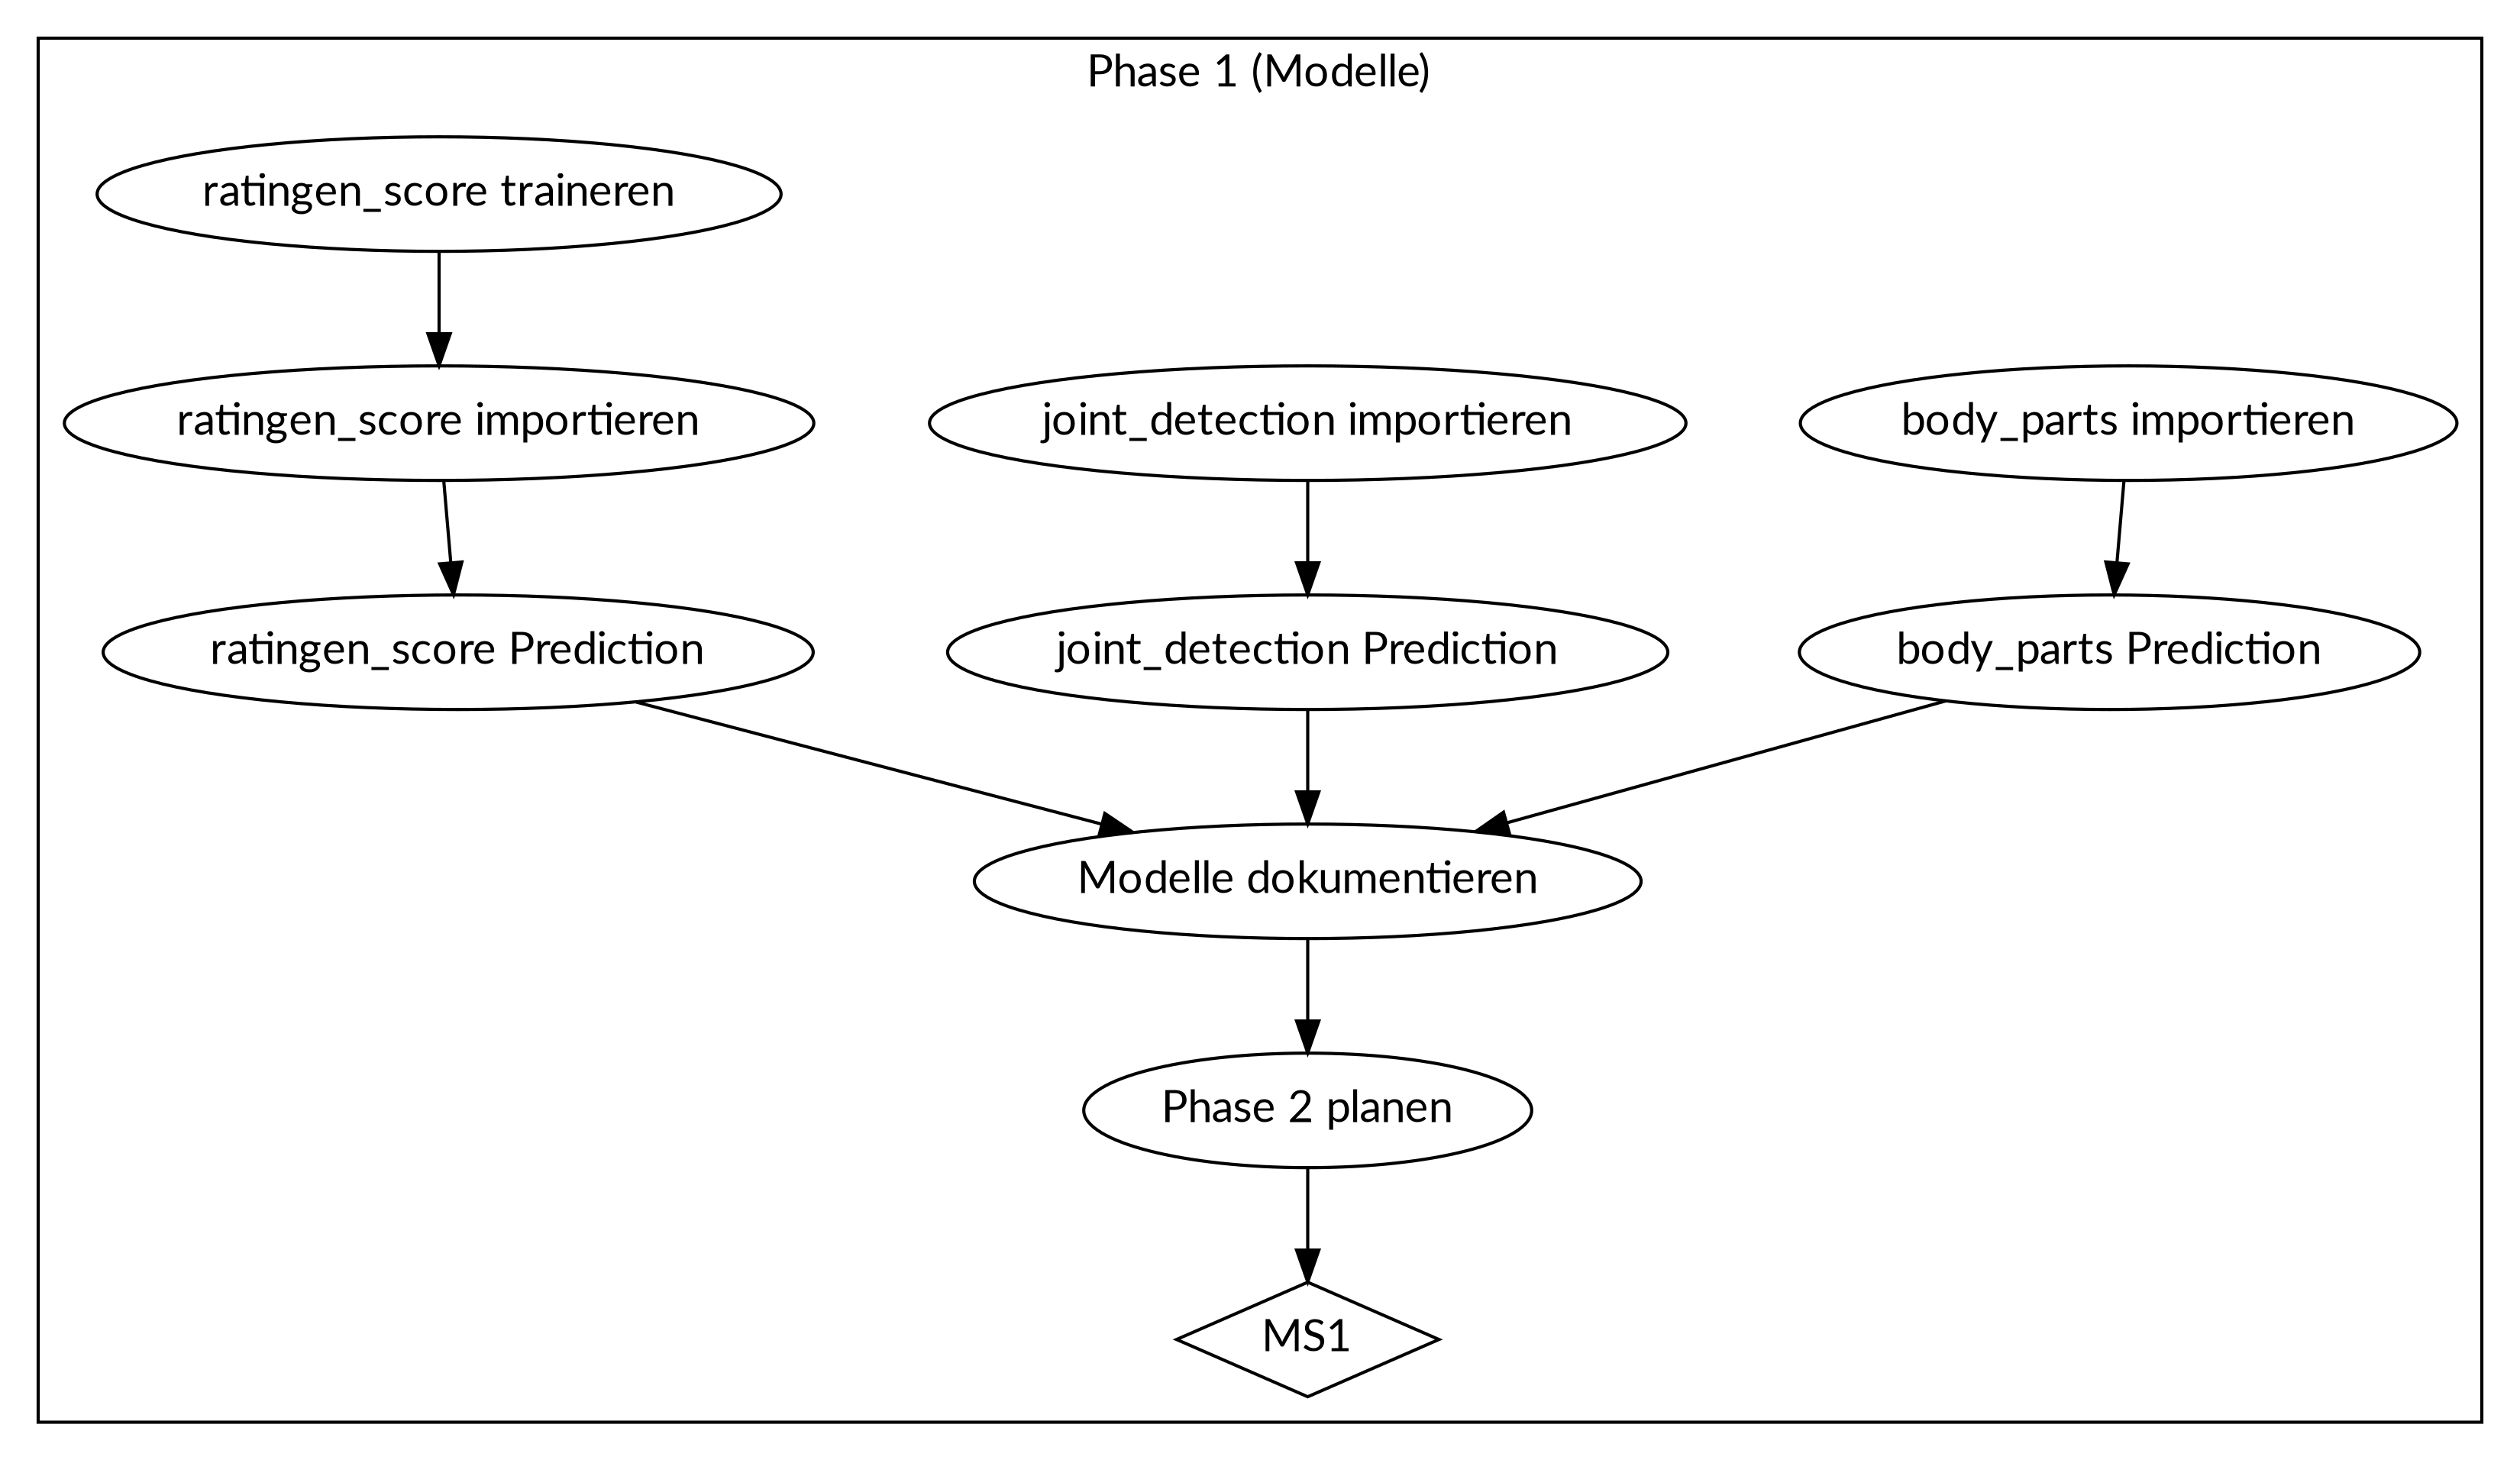
\includegraphics[width=\linewidth]{pics/phase1.png}
    \caption{In der ersten Projektphase werden die drei Modelle lauffähig gemacht und dokumentiert.}
    \label{fig:projekt-phase1}
\end{figure}

\paragraph{Reflexion}

Das Modell \texttt{ratingen\_score} konnte neu trainiert und erfolgreich exportiert werden. Alle drei Modelle sind in einer isolierten Umgebung (Docker-Container) lauffähig. Die Predictions der Modelle sind plausibel, wobei hierfür keine systematischen Tests vorgenommen worden sind. Die Laufzeitperformance erscheint als akzeptabel; die Predictions laufen in Sekundenschnelle ab.

\subsubsection{Zweite Phase: Architektur}

\begin{itemize}
    \item \textbf{Ziel:} Architektur und Evaluationsmetriken festlegen
    \item \textbf{Artefakte}
        \begin{enumerate}
            \item Architekturvorschläge und -diskussion
            \item begründeter Architekturentscheid
            \item Liste mit einzusetzenden Technologien
            \item Evaluationsmetriken
            \item Testkonzept
            \item Planung Phase 3
        \end{enumerate}
    \item \textbf{Aufgaben}
        \begin{enumerate}
            \item Architektur
                \begin{multicols}{2}
                    \begin{enumerate}
                        \item Integrationsvarianten finden
                        \item Architekturvorschläge aufstellen
                        \item Architekturvariante auswählen
                        \item Technologien finden
                        \item Prototyp implementieren
                    \end{enumerate}
                \end{multicols}
            \item Evaluation
                \begin{multicols}{2}
                    \begin{enumerate}
                        \item Datentypen finden
                        \item Datentypen der Modelle ermitteln
                        \item Evaluationsmetriken finden
                        \item Evaluationsmetriken bewerten
                        \item Geeignete Evaluationsmetriken auswählen
                    \end{enumerate}
                \end{multicols}
        \end{enumerate}
    \item \textbf{Risiken und Mitigationen}
        \begin{enumerate}
            \item Es lassen sich keine geeigneten Technologien für einen Architekturvorschlag finden.
                \begin{enumerate}
                    \item Es wird auf eine andere Architekturvariante ausgewichen.
                \end{enumerate}
            \item Der Prototyp kann mit der vorgeschlagenen Architekturvariante nicht umgesetzt werden.
                \begin{enumerate}
                    \item Es wird auf eine andere Architekturvariante ausgewichen.
                    \item Ein weiterer Prototyp wird implementiert, um die andere Variante zu prüfen.
                \end{enumerate}
            \item Es gibt keine geeigneten Evaluationsmetriken für das Gesamtsystem.
                \begin{enumerate}
                    \item Die Evaluation wird isoliert für die einzelnen Modelle vorgenommen.
                \end{enumerate}
        \end{enumerate}
\end{itemize}

\begin{figure}
    \centering
    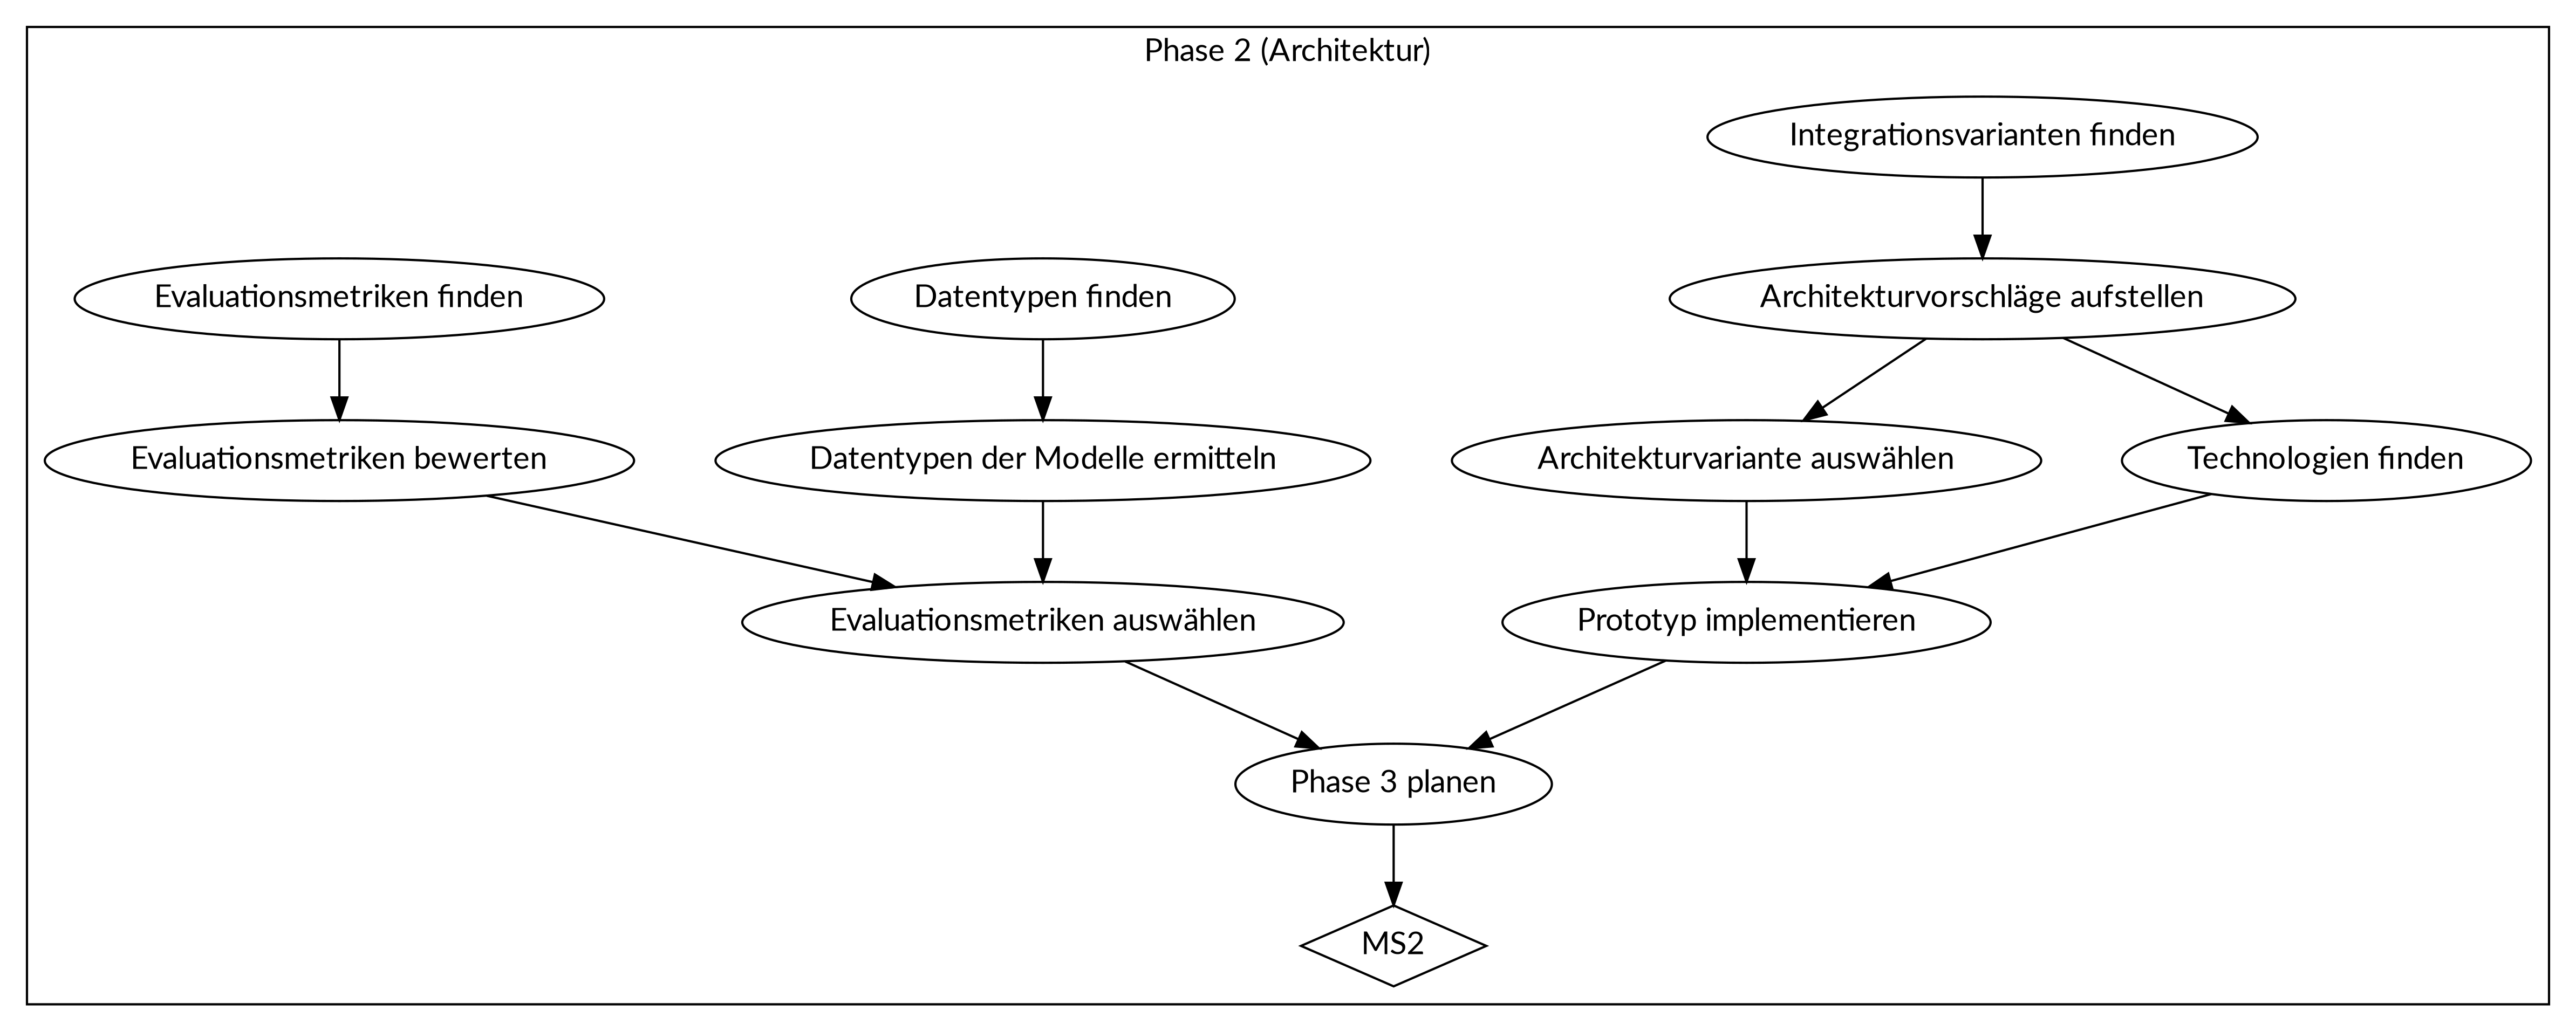
\includegraphics[width=\linewidth]{pics/phase2.png}
    \caption{In der zweiten Projektphase sollen Architekturvarianten und Evaluationsmetriken gefunden werden. Mithilfe eines Prototyps wird der Architekturvorschlag validiert.}
    \label{fig:projekt-phase2}
\end{figure}

\paragraph{Reflexion}

Das Auffinden verschiedener Integrationsvarianten, dazu passender Technologien und Evaluationsmetriken gestaltete sich sehr einfach. Hier war eher die Vielzahl der Möglichkeiten als deren Mangel ein Problem. Die Ausgestaltung und Auswahl der Architekturvarianten hat sehr viel Zeit in Anspruch genommen. Diese Investition hat sich jedoch gelohnt, zumal der Prototyp auf Anhieb funktioniert hat und als Vorlage für den zu erstellenden Webservice dienen kann.

\subsubsection{Dritte Phase: Orchestrierung}


\begin{itemize}
    \item \textbf{Ziel:} lauffähiger Prototyp mit Evaluationsergebnissen
    \item \textbf{Artefakte}
        \begin{enumerate}
            \item ausführbarer Programmcode
            \item ausführbare Testfälle
            \item gelabelte Evaluationsdaten
            \item Evaluationsworkflow (Programmcode)
            \item Evaluationsergebnisse
        \end{enumerate}
    \item \textbf{Aufgaben}
        \begin{enumerate}
            \item Webservice-Prototyp
                \begin{multicols}{2}
                    \begin{enumerate}
                        \item \texttt{body\_part} umsetzen
                        \item \texttt{joint\_detection} umsetzen
                        \item \texttt{ratingen\_score} umsetzen
                        \item \texttt{orchestrator} umsetzen
                        \item Web-UI umsetzen
                    \end{enumerate}
                \end{multicols}
            \item Evaluation
                \begin{multicols}{2}
                    \begin{enumerate}
                        \item Evaluationsdaten selektieren
                        \item Evaluationsdaten aufbereiten
                        \item Evaluationsdaten scoren
                        \item Evaluationsworkflow umsetzen
                        \item Ergebnisse evaluieren
                    \end{enumerate}
                \end{multicols}
        \end{enumerate}
    \item \textbf{Risiken und Mitigationen}
        \begin{enumerate}
            \item Der Webservice läuft zu langsam.
                \begin{enumerate}
                    \item Es soll eine performantere Laufzeitumgebung verwendet werden.
                    \item Die geringe Performance soll analysiert, Verbesserungsvorschläge sollen im Ausblick dokumentiert werden.
                \end{enumerate}
            \item Die asynchrone Architektur führt zu inkonsistenten Ergebnissen (Vermischung der Resultate).
                \begin{enumerate}
                    \item Es sollen zuverlässige Synchronisationsmassnahmen eingesetzt werden.
                    \item Es kann auf eine synchrone Architektur ausgewichen werden.
                \end{enumerate}
            \item Es stehen keine oder zu wenige Evaluationsdaten zur Verfügung.
                \begin{enumerate}
                    \item Der Evaluationsworkflow wird nur mit Platzhalterdaten ausgeführt. Die Evaluationsergebnisse sollen zu einem späteren Zeitpunkt vom Auftraggeber ermittelt werden.
                \end{enumerate}
            \item Die Evaluationsdaten lassen sich nicht in nützlicher Frist verarbeiten.
                \begin{enumerate}
                    \item Es soll nur eine Untermenge der Evaluationsdaten verarbeitet werden.
                \end{enumerate}
            \item Die Evaluationsergebnisse sind unbefriedigend (schlechte Performance).
                \begin{enumerate}
                    \item Dieses Risiko ist für den Auftraggeber zu tragen, da die Modelle (und somit die Prediction-Performance) vorgegeben waren.
                \end{enumerate}
        \end{enumerate}
\end{itemize}

\begin{figure}[tbh]
    \centering
    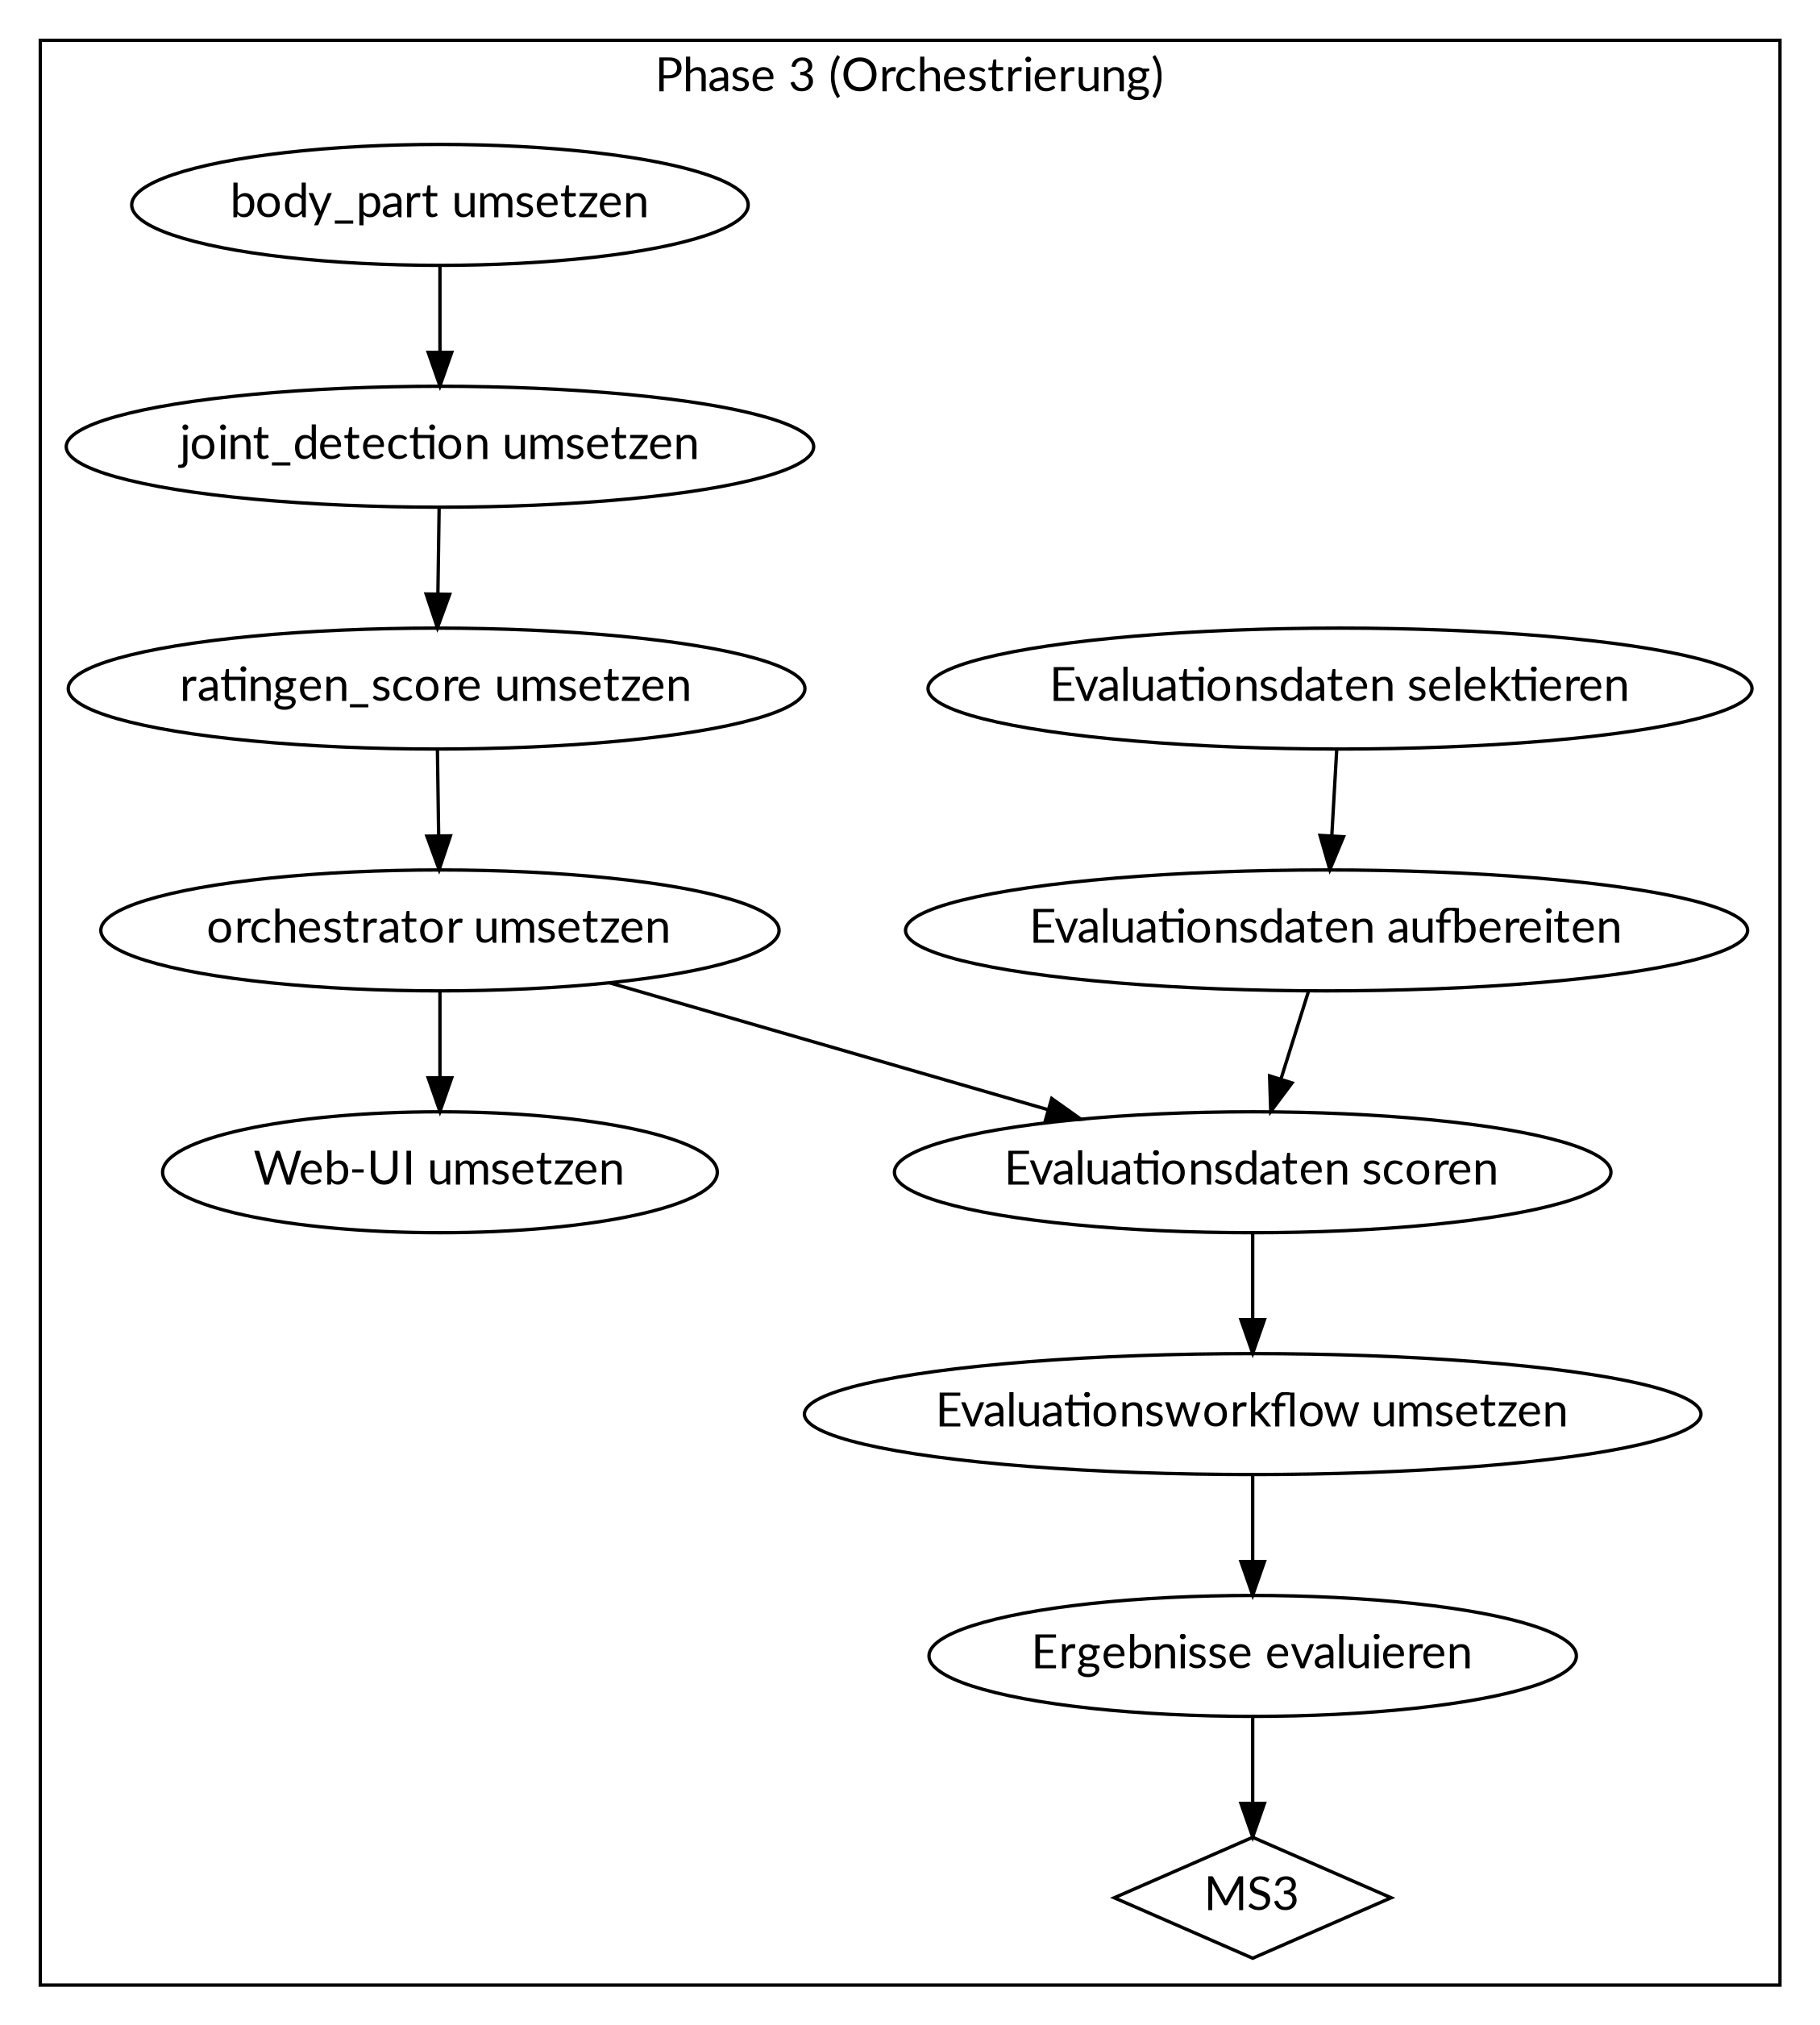
\includegraphics[width=0.7\linewidth]{pics/phase3.png}
    \caption{In der dritten Projektphase werden die einzelnen Teile zu einem lauffähigen System kombiniert. Dieses wird mit ausgewählten Metriken und entsprechenden Daten evaluiert.}
    \label{fig:projekt-phase3}
\end{figure}

\paragraph{Reflexion}

Der Prototyp aus Phase 2 hat sich als Glücksfall erwiesen, zumal der Webservice analog zu ihm umgesetzt werden konnte. Mit den gewählten Technologien (Go, RabbitMQ, Docker) konnte der Webservice erstaunlich schnell umgesetzt werden ‒ und lässt sich ohne Änderungen auf verschiedenen Umgebungen ausführen. Die Laufzeitperformance des Gesamtsystems ist für einen Prototyp akzeptabel, für den Produktiveinsatz jedoch verbesserungswürdig. Es konnten (in teilweise manueller Arbeit) genügend Evaluationsdaten gesammelt werden, um damit den Evaluationsworkflow umzusetzen und angemessen auf Plausibilität testen zu können. Für eine aussagekräftige Evaluation wären jedoch noch weitere ungesehene Daten nötig.

\subsubsection{Meilensteinplanung}

Die Meilensteinplanung (siehe \tblref{tbl:meilensteinplanung}) deckt sich grösstenteils mit der Projektphasenplanung, zumal am Ende einer jeden Projektphase ein Meilenstein erreicht werden soll. Als vierter und entscheidender Meilenstein kommt die Schlussabgabe hinzu, bei der zusätzlich die Artefakte Bericht, Web-Abstract und Pitching-Video abzuliefern sind.

\begin{table}[tbh]
    \center
    \small{
        \begin{tabular}{r|r|l|l}
            MS & SW & Datum & Beschreibung \\ \hline
            1 & 6 & 31.03.2020 & Phase 1 (Modelle) abgeschlossen \\
            2 & 8 & 19.04.2020 & Phase 2 (Architektur) abgeschlossen \\
            3 & 13 & 24.05.2020 & Phase 3 (Orchestrierung) abgeschlossen \\
            4 & 15 & 05.06.2020 & Schlussabgabe \\
        \end{tabular}
    }
    \caption{In der Meilensteinplanung wird neben den drei detailliert geplanten Projektphasen auch die Schlussabgabe als vierter Meilenstein berücksichtigt.}
    \label{tbl:meilensteinplanung}
\end{table}

\subsubsection{Wochenplan}

Obwohl in der Projektplanung (siehe \secref{sec:projektphasen}) auf eine detaillierte zeitliche Planung der einzelnen Aufgaben innerhalb der verschiedenen Projektphasen verzichtet worden ist, soll der Wochenplan (siehe \tblref{tbl:wochenplanung}) eine zusätzliche zeitliche Orientierung ermöglichen. Im Gegensatz zum Meilensteinplan ist im Wochenplan auch die Erstellung der Schlusspräsentation berücksichtigt, welche in den Wochen nach der Abgabe erfolgen soll.

\begin{table}[tbh]
    \small{
        \begin{tabularx}{\textwidth}{r|r|r|X|X}
            SW & Von & Bis & Tätigkeiten & Ereignis/Meilenstein \\ \hline
            0 & 12.02. & 16.02. & Projektinitialisierung (Kick-Off) & Projektstart \\
            1 & 17.02. & 23.02. & Recherche, Bestandesaufnahme & \\
            2 & 24.02. & 01.03. & Recherche, Import bestehender Modelle & \\
            3 & 02.03. & 08.03. & Recherche, Import bestehender Modelle & \\
            4 & 09.03. & 15.03. & Recherche, Projektplanung & Erteilung def. Projektauftrag \\
            5 & 16.03. & 22.03. & Import/Ausführung bestehender Modelle & \\
            6 & 23.03. & 29.03. & Import/Ausführung bestehender Modelle, Dokumentation & \\
            7 & 30.03. & 05.04. & Dokumentation, Planung, Architektur & MS1 \\
            8 & 06.04. & 12.04. & Architektur & \\
            9 & 13.04. & 19.04. & Architektur, Dokumentation, Planung & MS2 \\
            10 & 20.04. & 26.04. & Umsetzung, Dokumentation & Zwischenpräsentation \\
            11 & 27.04. & 03.05. & Umsetzung, Dokumentation & \\
            12 & 04.05. & 10.05. & Umsetzung, Dokumentation & \\
            13 & 11.05. & 17.05. & Umsetzung, Dokumentation & \\
            14 & 18.05. & 24.05. & Deployment, Dokumentation & MS3, lauffähiger Prototyp \\
            15 & 25.05. & 31.05. & Dokumentation, Video & \\
            16 & 01.06. & 05.06. & Abschliessen Dokumentation & Schlussabgabe \\
            & 06.05. & 30.06. & Abschlusspräsentation erstellen & Abschlusspräsentation \\
        \end{tabularx}
    }
    \caption{Der Wochenplan dient ‒ als Ergänzung zu Phasen- und Meilensteinplan ‒ als zeitliche Orientierungshilfe für den Projektablauf.}
    \label{tbl:wochenplanung}
\end{table}

\clearpage

\subsection{Teststrategie}
\label{sec:teststrategie}

Wie bereits im Modul \textit{Software Testing} (Frühlingssemester 2019) eingeübt und im \textit{Wirtschaftsprojekt} (Herbstsemester 2019) gewinnbringend eingesetzt, sollen die \textit{Agile Test Quadrants} (\imgref{fig:agile-testing-quadrants}) wiederum als Grundlage für die Erarbeitung einer Teststrategie dienen.\footnote{Auf die Umsetzung der Tests wird erst im Folgekapitel \secref{sec:realisierung} eingegangen.}

\begin{figure}[tbh]
    \centering
    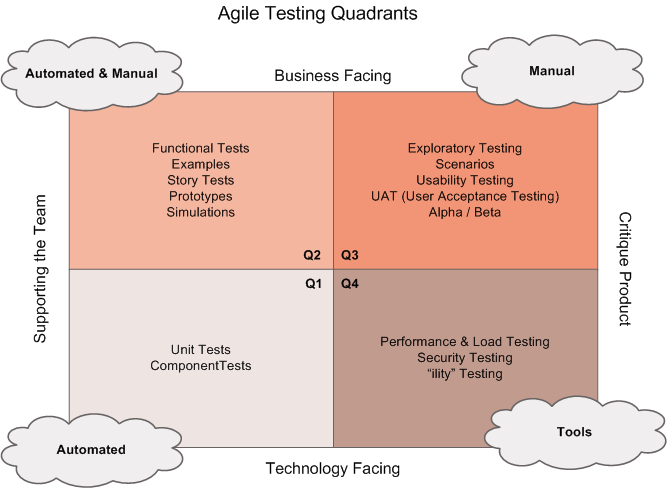
\includegraphics[width=\linewidth]{pics/agile-testing-quadrants.png}
    \caption{Die \textit{Agile Testing Quadrants} (\url{https://lisacrispin.com/2011/11/08/using-the-agile-testing-quadrants}) sind eine bewährte Orientierungshilfe für das Erarbeiten einer Teststrategie.}
    \label{fig:agile-testing-quadrants}
\end{figure}

Die verschiedenen Arten von Tests werden dabei als Werkzeuge betrachtet, die man für geeignete Aufgaben einsetzt ‒ und für weniger geeignete Aufgaben wieder in die Werkzeugkiste zurücklegt. Die Wahl der Testwerkzeuge soll pragmatisch erfolgen, d.h. im Hinblick auf ihre Effektivität (ein Systemmerkmal wird sinnvoll geprüft) und Effizienz (mit wenig Testcode kann viel produktiver Code abgedeckt werden). Eindimensionale Metriken wie \textit{«Es soll 95\% des Codes mit Unittests abgedeckt werden»} lesen sich bei diesem Verständnis wie \textit{«Der Bau der Hundehütte soll weitgehendst mit dem Hammer erfolgen»}. \footnote{Mit den Einfluss der Werkzeuge auf das Denken hat sich u.a. Edsger W. Dijkstra befasst \cite{dijkstra-council}. Das Zitat, \textit{«If your only tool is a hammer, then every problem looks like a nail.»}, dessen Ursprung umstritten ist \cite{quoteinvestigator}, veranschaulicht das Problem pointiert.} 

Die vier Quadranten, und ihre möglichen Anwendungen für das vorliegende Projekt \textit{DeepXRay}, werden im Folgenden beschrieben.

\subsubsection{Q1: automatisiert}

Im ersten Quadranten geht es um Unittests und Komponententests. Diese sollen v.a. für den neu zu erstellenden Code geschrieben werden, der keine Abhängigkeit zu anderen Laufzeitkomponenten hat. Beim bestehenden Code (Modelle) ist dies nur teilweise sinnvoll, zumal es sich dabei um Legacy-Code handelt, der eher abgelöst als erweitert werden soll. Beim \texttt{orchestrator}, der viele Abhängigkeiten zu anderen Laufzeitkomponenten hat, wären solche Tests nur über umfassendes und aufwändiges \textit{Mocking} möglich.\footnote{Beim Mocking wird häufig die interne Funktionsweise des Testcodes simuliert. Hierzu ist nicht nur Kenntnis der Schnittstelle, sondern auch der Implementierung vonnöten. Unittests, die Mocking verwenden, sind daher häufig fragil ‒ und strenggenommen keine Black-Box-Tests. Mocking, bzw. dessen Notwendigkeit für das Schreiben von Unittests, gilt daher teilweise als \textit{Code Smell} \cite[S. 214]{composing-software}.} Der Evaluationsworkflow hingegen, bei dem verschiedene mathematische Metriken implementiert werden müssen, lässt sich hervorragend mittels Unittests prüfen.

Für den Evaluationscode soll auch die Testabdeckung gemessen werden. Absolute Ziele (z.B. \textit{«95\% der Codezeilen durch Testfälle abgedeckt»}) sind dabei wenig hilfreich, da man eine hohe Codeabdeckung auch erreichen kann, ohne die Ergebnisse zu überprüfen, die vom jeweiligen Code zurückgeliefert werden. Vielmehr geht es beim Messen der Testabdeckung darum, auf Codepassagen aufmerksam zu werden, die nicht automatisiert getestet werden.

\subsubsection{Q2: automatisiert und manuell}

Im zweiten Quadranten geht es um Tests, die manuell durchgeführt, bei Bedarf aber auch automatisiert werden können.

Das Vorgehen im Wirtschaftsprojekt im letzten Herbst hat sich dabei als sehr sinnvoll erwiesen: Tests werden zunächst manuell durchgeführt. Erst wenn man bemerkt, dass ein und derselbe Test immer wieder durchgeführt werden muss ‒ und das Testen die Hände stärker beansprucht als den Kopf ‒, wird der Test mithilfe eines Testskripts automatisiert. So leistet man nur dort Automatisierungsarbeit, wo diese wirklich sinnvoll ist.

Im vorliegenden Projekt könnten folgende Arten von Tests sinnvollerweise automatisiert werden:

\begin{description}
    \item[Tests der einzelnen Modelle] Da die Erstellung der Modelle nicht Bestandteil der Arbeit ist, werden die Modelle nicht auf Performance im Sinne «korrekter» Predictions geprüft. Es geht vielmehr darum zu prüfen, ob das Modell auch von aussen ansprechbar ist und soweit «korrekt» arbeitet, wie es eben erstellt worden ist. Hierzu können Sammlungen von Testdaten erstellt werden, die Inputs zu Outputs mappen. Dies könnte etwa folgendermassen aussehen:
        \begin{itemize}
            \item \texttt{body\_part}: Ein Bild (Input) wird zu einem String (erkanntes Körperteil) gemappt.
            \item \texttt{joint\_detection}: Ein Bild (Input) wird zu zehn anderen Bildern (extrahierte Gelenke) ‒ oder zu einer Fehlermeldung, falls keine Gelenke erkannt worden sind, ‒ gemappt.
            \item \texttt{ratingen\_score}: Ein kleines Bild von einem Gelenk, das aus einer Röntgenaufnahme extrahiert worden ist, wird zu einer Score gemappt.
        \end{itemize}
    \item[Tests über das ganze System] Hierbei können die Testdefinitionen der einzelnen Modelle wiederverwendet werden, indem etwa ein ganzes Röntgenbild (Input) zu einer Reihe von Scores (oder zu einer Fehlermeldung) gemappt wird.
\end{description}

Für diese Testdefinitionen ist ein sinnvolles Format zu definieren. Eine Möglichkeit wäre JSON-Dateien, die einen Dateinamen zu einem Output mappen. Diese JSON-Dateien könnten statt Dateinamen auch die eigentlichen Bilddaten enthalten, indem diese base64-kodiert direkt eingefügt werden. Beim ersten Ansatz wird das manuelle Betrachten von Testinputs einfacher. Im zweiten Ansatz sind die Testdaten schöner abgekapselt.

In jedem Fall muss ein Testrunner entwickelt werden, der mit den definierten Testdaten umgehen kann. Je nach verwendeter Schnittstelle sieht ein solcher Testrunner anders aus. Mit dem Python-Testframework PyTest und der Testing-Library von Go konnten dabei schon viele positive Erfahrungen gesammelt werden.

Um die nebenläufige Verarbeitung von Röntgenbildern testen zu können, soll ein (nicht-deterministischer) Testfall erstellt werden, der mehrere Röntgenbilder schnell nacheinander zur Verarbeitung übergibt, ohne die eintreffenden Antworten synchron abzuwarten. Diese werden nebenläufig eingesammelt. Die Antworten sind darauf zu prüfen, dass sie immer die gleichen Scores pro Röntgenbild enthalten. So kann (mit hoher Wahrscheinlichkeit) sichergestellt werden, dass der \texttt{orchestrator} die einzelnen Vorgänge intern korrekt auseinanderhält.

\subsubsection{Q3: manuell}

Der dritte Quadrant spielt im Rahmen der vorliegenden Arbeit nur eine sehr untergeordnete Rolle. Da die grafische Benutzeroberfläche, die für den Prototyp erstellt wird, nur zu Demozwecken dienen soll und kein eigentliches Lieferobjekt des vorliegenden Projekts ist, erübrigen sich formalisierte Tests desselben.

Manuelle Tests könnten sich aber an andere Stakeholder richten und sich auf die Umgebung des Prototyps beziehen.

\begin{itemize}
    \item Wie kann die Umgebung in Betrieb genommen werden?
    \item Wie können die Testfälle ausgeführt werden?
    \item Wie finde ich Hilfe (Dokumentation), wenn etwas nicht (mehr) funktioniert?
\end{itemize}

Rückmeldungen in diesem Bereich sind gerade im Hinblick auf die Abgabe des Projekts sinnvoll, und könnten vom Auftraggeber und vom Betreuer eingeholt werden.

\subsubsection{Q4: Tools}

Im vierten Quadranten geht es v.a. um das Testen nicht-funktionaler Anforderungen, d.h. Performance, Security, Usability usw. Da es im vorliegenden Projekt nur um die Entwicklung eines Prototyps geht, können Überlegungen zu den Aspekten Security und Usability von Beginn weg weitgehend ausgeklammert worden.

Die Verarbeitung von Röntgenbildern kann mit einem Benchmark im Bezug auf die Laufzeitperformance untersucht werden. Go bietet hierfür passende Funktionalität in der Standardbibliothek \cite[Kapitel 11.4]{gopl}.

Flaschenhälse bei der Performance (CPU, Memory, I/O) könnten per Profiling ermittelt werden. Eine umfassende Analyse des Laufzeitverhaltens mittels Profiling ist jedoch aufwändig und soll nicht im Rahmen des vorliegenden Projekts erfolgen.

Für die Codequalität ist es sinnvoll, wenn statische Codeanalyse verwendet wird. Sogenannte Linter führen auf Basis von Regeln und Heuristiken Codeüberprüfungen durch und geben Warnungen bei potenziellen Problemen ab, die meist stilistischer Natur sind. Mögliche Werkzeute sind \texttt{pylint} (Python) und \texttt{golint} (Go). Code-Auditing-Tools wie \texttt{py\-lama} (Python) und \texttt{go vet} (Go) warnen den Programmierer vor möglichen Problemen und Fehlern, und sollten darum auch eingesetzt werden, idealerweise automatisiert und in der Entwicklungsumgebung integriert.

Bei der Verwendung von Tools ist es wichtig, dass diese einfach eingesetzt werden können. Im Wirtschaftsprojekt hat sich ein einfaches \texttt{Makefile} als gute Variante erwiesen. Mit Befehlen wie \texttt{make cover} wurden etwa alle Unittests ausgeführt und die Codeabdeckung ausgegeben. Müsste man den ganzen Befehl dafür jeweils von Hand eintippen oder in der Shell-History suchen, wäre der Aufruf entsprechend umständlicher.

\subsubsection{Testumgebung}

Wie der zu erstellende Prototyp sollen die Tests zunächst nur auf einer Test- bzw. Demoumgebung ausführbar sein. Bei Seantis wird die CI-Umgebung Buildkite\footnote{\url{https://buildkite.com/} (abgerufen am 17.05.2020)} verwendet, die sich nur mit grösserem Aufwand für neue Projekte einrichten lässt, zumal die erstellten Container für die Modellkomponenten dem CI-System über das interne Container-Buildtool \texttt{parts} zugänglich gemacht werden müssten.

Die Integration in die CI-Umgebung des Auftraggebers soll darum nicht Bestandteil des vorliegenden Projekts sein.

\newpage

\section{Realisierung}
\label{sec:realisierung}

Beschreiben die bisherigen Kapitel, wie der Prototyp aufgebaut werden \textit{soll}, geht es in diesem Kapitel darum, was tatsächlich umgesetzt worden \textit{ist}. Der Prototyp basiert auf der Architekturvariante, die in \secref{sec:variante-4-messaging} beschrieben worden ist.

Als Messaging-Lösung kommt RabbitMQ mit dem AMQP-Protokoll zum Einsatz (siehe \secref{sec:wahl-der-message-queue}).

Die Quellcodeartefakte und Modelldaten befinden sich im Abgabeordner (\texttt{Zusatz/}) im Unterverzeichnis \texttt{deepxray/}.

\subsection{Modellkomponenten}

Die bestehenden Machine-Learning-Modelle wurden im Abschnitt \secref{sec:bestehende-modelle} in ihrer Funktionsweise grob beschrieben. Die eigentlichen Modelle werden um weiteren Code ergänzt, wodurch diese mit der Aussenwelt interagieren können. Die Kombination aus den eigentlichen Modellen und dem zusätzlichen Code zur Interaktion mit der Aussenwelt ‒ der \textit{Integrationscode} ‒ wird als \textit{Modellkomponente} bezeichnet. Für Komponente und Modell werden die gleichen Bezeichnungen verwendet; ob das Modell oder die Modellkomponente gemeint ist, ergibt sich dabei aus dem Kontext. Sämtliche Modellkomponenten sind in Python geschrieben (siehe \secref{sec:wahl-der-programmiersprache-modellkomponenten}).

Die Modellkomponenten wurden alle nach dem gleichen Schema aufgebaut, wobei die Extraktion der Gelenke (\texttt{joint\_detection}) aufgrund der zehn verschiedenen Modelle etwas aus der Reihe tanzt.

Für jede Modellkomponente gibt es eine \textit{Hauptklasse}, die den jeweiligen Einstiegspunkt (Hauptprogramm) für die Komponente darstellt. Dazu kommt eine \textit{Predictor}-Klasse, die das Machine-Learning-Modell kapselt und ein Interface für dieses anbietet. Die Hauptklasse kümmert sich um die Kommunikation mit der Message-Queue. Eingehende Nachrichten werden für den Predictor aufbereitet. Es folgt der Aufruf des Predictors, der das Ergebnis an die Hauptklasse zurückliefert. Hier wird die Antwort interpretiert (Erfolg oder Fehler) und an die entsprechende Message-Queue weitergeleitet.

Innerhalb der Modellkomponenten erfolgt die Abarbeitung synchron: Von der eingehenden Queue wird jeweils nur eine Message geholt und verarbeitet. Erst dann wird die nächste Message entgegengenommen und wiederum verarbeitet. Die parallele Verarbeitung erfordert somit, dass mehrere Instanzen pro Modellkomponente am Laufen sind.

\subsubsection{Aufbau der Modellkomponenten}
\label{sec:aufbau-der-modellkomponenten}

Diese verallgemeinerte Struktur wird im Klassendiagramm auf \imgref{fig:klassendiagramm-generisch} veranschaulicht. Die Hauptklasse (\texttt{Main}) verfügt jeweils über eine Verbindung mit dem Message-Broker (\texttt{connection}) und einen Kanal (\texttt{channel}), der über diese Verbindung kommuniziert. Eine \texttt{Predictor}-Instanz wird im Konstruktor der \texttt{Main}-Klasse erzeugt. Im Konstruktor (\texttt{\_\_init\_\_()}) der \texttt{Predictor}-Klasse wird das eigentliche Modell geladen. Hierzu wird ein Modellpfad benötigt, den die \texttt{Main}-Klasse aus einer Umgebungsvariablen liest.

\begin{figure}[tbh]
    \centering
    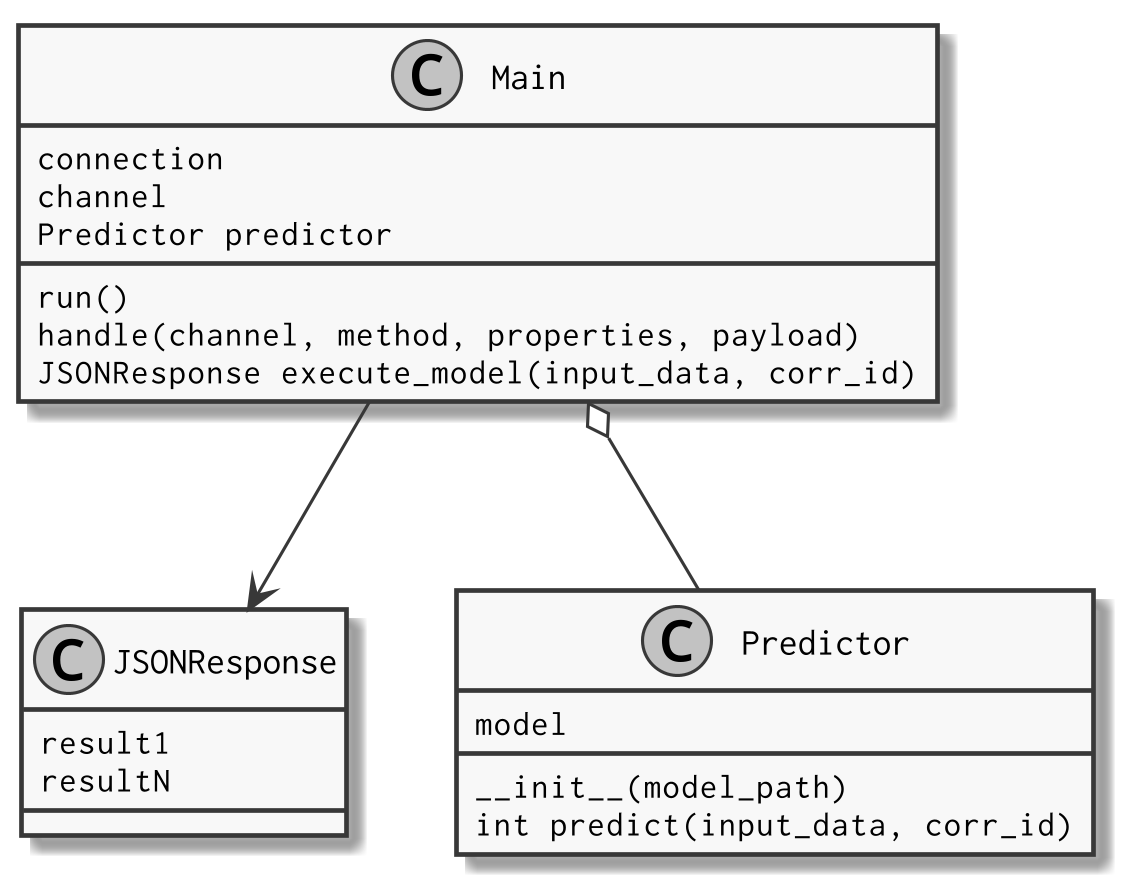
\includegraphics[width=0.9\linewidth]{pics/class-generic.png}
    \caption{Die allgemeine Architektur der Modellkomponenten, bestehend aus einer Hauptklasse und einer Predictor-Klasse. (Klassendiagramm)}
    \label{fig:klassendiagramm-generisch}
\end{figure}

Die \texttt{run()}-Methode wird vom Hauptprogramm aufgerufen, sobald die Klasse instanziiert ist. Diese stellt sicher, dass alle benötigten Queues vorhanden sind, registriert die Callback-Methode für eingehende Nachrichten (\texttt{handle()}), und lässt anschliessend auf eingehende Nachrichten warten.

Die \texttt{handle()}-Methode wird automatisch aufgerufen, sobald eine Nachricht aus der Queue eintrifft. Diese hat per API-Definition vier Parameter: Der \texttt{channel} wird dazu benötigt, um Nachrichten aus dem Callback heraus zu publizieren (etwa um Antworten zu senden). Der Parameter \texttt{method} ist ein AMQP-Delivery-Object, welches hier dazu dient, die Verarbeitung der Nachricht zu bestätigen, um darauf die nächste Nachricht zu erhalten. Der \texttt{properties}-Parameter enthält verschiedene Informationen, wovon hier nur der Correlation Identifier (\texttt{corr\_id}) relevant ist. Dieser wird benötigt, um ausgehende Nachrichten dem gleichen Vorgang zuzuordnen wie die eingegangene Nachricht.\footnote{Das Konzept des Correlation Identifiers wird in Abschnitt \secref{sec:variante-3-messaging} erklärt.} Der \texttt{body}-Parameter schliesslich enthält den Payload der Nachricht, sprich die eigentlichen Nutzdaten.

Beim Payload handelt es sich meistens um eine JSON-Datenstruktur. Diese enthält ein Bild (ganzes Röntgenbild oder nur einen einzelnen Gelenkausschnitt davon) und im Falle der Extraktion und des Scorings noch eine Gelenkbezeichnung. Das Bild ist jeweils als base64-kodierte Zeichenkette abgelegt.\footnote{Dieses Austauschformat wurde aufgrund früherer positiver Erfahrung in verschiedenen Projekten gewählt, ohne dass hierzu ausführlich Alternativen geprüft worden sind. \textit{Protocol Buffers} dürften aufgrund des binären Übertragungsformats eine höhere Effizienz ermöglichen, jedoch auch eine höhere Komplexität ‒ eine zusätzliche Notation und einen weiteren Build-Schritt ‒ mit sich bringen \cite{protobuf}. Zudem erschien es dem Autor dieser Arbeit vernünftiger, die Anzahl der für ihn neuen Technologien und Konzepte ‒ Machine Learning, Messaging via AMQP ‒ innerhalb eines Projekts nicht weiter auszudehnen. Die Codierung, Übertragung und Dekodierung der Bilder stellt auch bei Weitem nicht den Flaschenhals in der Verarbeitung dar, wodurch der Einsatz von Protocol Buffers wohl kaum spürbare Performanceauswirkungen auf das Gesamtsystem hätte.} Das Bild wird dekodiert und ‒ wenn nötig mit Zusatzinformationen; zwecks Logging immer mit dem Correlation Identifier (\texttt{corr\_id})  ‒ an die \texttt{execute\_model()}-Methode übergeben. Diese kapselt den Aufruf der \texttt{predict()}-Methode der \texttt{Pre\-dictor}-Instanz.

Die \texttt{predict()}-Methode führt die Prediction auf Basis des Modells aus, wovor teilweise noch einzelne Verarbeitungsschritte zu erfolgen haben (\textit{Preprocessing}). Die ermittelte Prediction (der Output des Modells) wird von der Methode zurückgeliefert. Dieser wird von der \texttt{execute\_model()}-Methode in eine JSON-Struktur (im Klassendiagramm als \texttt{JSONRe\-sponse} bezeichnet\footnote{Diese Klasse ist rein konzeptionell zu verstehen. Tatsächlich findet sich in keiner der drei Modellkomponenten eine Python-Klasse dieses Namens. Es handelt sich vielmehr jeweils um ein Dictionary (\texttt{dict}), das die aufgelisteten Eigenschaften enthält. Eine Implementierung in Java würde hier tendenziell eine Klasse verwenden, bei Go dürfte eine Struktur zum Einsatz kommen.}) verpackt und an die \texttt{handle()}-Methode zurückgegeben, welche diese wiederum als Payload an die Ergebnis-Queue weitergibt. Tritt in diesem Prozess ein Fehler auf, wird von \texttt{predict()} eine entsprechender Exception geworfen, der erst von \texttt{handle()} abgefangen und als Fehlermeldung an die Fehler-Queue weitergereicht wird.

Dieser Prozess beschreibt die Arbeitsweise der Modellkomponenten im Allgemeinen. In den folgenden Abschnitten für die einzelnen Modellkomponenten wird nur noch auf Erweiterungen und Abweichungen dieses allgemeinen Schemas eingegangen. Auf weitere gemeinsame Aspekte, die eher technischer Natur sind, wird im Abschnitt \secref{sec:gemeinsame-technische-aspekte} eingegangen, der als Anhang zu diesem Unterkapitel zu lesen ist.

\subsubsection{Modellkomponente \texttt{body\_part}}
\label{sec:modellkomponente-body-part}

Das Erkennen eines Körperteils ist der erste Schritt in der Verarbeitung eines Röntgenbildes, bei dem ein Machine-Learning-Modell zum Einsatz kommt. Das Klassendiagramm dieser Komponente (siehe \imgref{fig:klassendiagramm-body-part}) entspricht dabei weitgehend demjenigen der generischen Modellkomponente.

\begin{figure}[tbh]
    \centering
    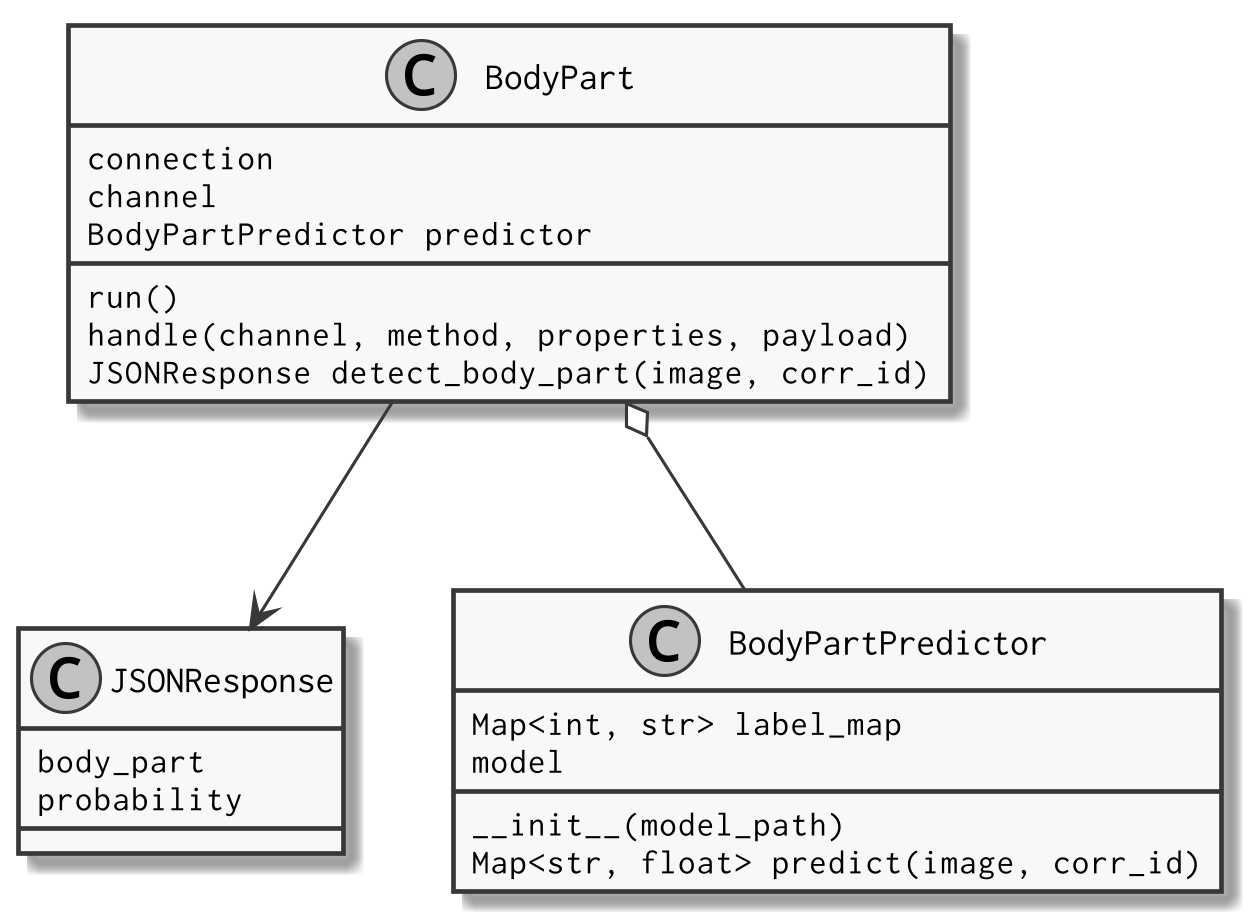
\includegraphics[width=0.9\linewidth]{pics/class-body-part.png}
    \caption{Die Modellkomponente \texttt{body\_part} entspricht in ihrer Klassenstruktur weitgehend der generischen Modellkomponente. (Klassendiagramm)}
    \label{fig:klassendiagramm-body-part}
\end{figure}

Die Unterschiede zur generischen Komponente liegen bei Input und Output von \texttt{body\_part}. Auf einem Röntgenbild (Input) wird erkannt, um welches Körperteil es sich mit welcher Wahrscheinlichkeit handelt. Die Körperteile werden mithilfe der \texttt{label\_map} in \texttt{BodyPartPredictor} zu den numerischen Outputs gemappt (das Label \texttt{hand left} hat den Output 6). Die \texttt{predict()}-Methode gibt eine Map von Körperteilen mit Wahrscheinlichkeiten zurück. In \texttt{detect\_body\_part()} wird dann das Körperteil mit der höchsten erzielten Wahrscheinlichkeit ausgewählt. Körperteil und Wahrscheinlichkeit werden zurückgegeben, damit letztere gegen eine vordefinierte Schwelle (z.B. mindestens 50\% Wahrscheinlichkeit) geprüft werden könnte.

Beide Informationen ‒ erkanntes Körperteil und Wahrscheinlichkeit ‒ werden mit der \texttt{JSONResponse} an den Client zurückgeliefert, damit dieser eine allfällige Schwellenwertprüfung selber durchführen könnte.

Die \texttt{run()}-Methode der \texttt{BodyPart}-Klasse konsumiert Nachrichten von einer Queue namens \texttt{body\_part}. Als Payload werden rohe JPEG-Daten (eine Reihe von Bytes) erwartet; eine Einbettung in JSON mit base64-Kodierung entfällt hier. Resultate werden auf einer Queue namens \texttt{body\_part\_response} publiziert.

Die Klasse \texttt{BodyPartPredictor} wird mit dem Integrationstest (\texttt{test\_body\_part\_pre\-dic\-tor.py}) im \texttt{tests/}-Unterverzeichnis getestet. Dieser prüft für verschiedene Röntgenbilder einer linken Hand, ob diese korrekt als das wahrscheinlichste Körperteil erkannt wird, und dass die Wahrscheinlichkeit in einem Bereich zwischen 0 und 1 liegt (Plausibilität). Für eine Röntgenaufnahme eines linken Fusses wird geprüft, dass auf dem Bild \textit{nicht} eine linke Hand erkannt wird.

\subsubsection{Modellkomponente \texttt{joint\_detection}}

Die Extraktion der Gelenke ist der aufwändigste Arbeitsschritt in der Verarbeitung von Röntgenbildern. Für jedes der zehn relevanten Gelenke (MCP 1-5, PIP 1-5) wird ein separates Modell benötigt. Eine \texttt{Predictor}-Klasse, die ein Modell lädt und verwendet, genügt bei der Modellkomponente \texttt{joint\_detection} nicht den Anforderungen.

Die einzelnen Modelle werden daher nicht über die \texttt{Predictor}-Klasse (\texttt{JointDetection\-Predictor}) abstrahiert, sondern über eine gesonderte \texttt{Model}-Klasse namens \texttt{Joint\-De\-tec\-tion\-Model}. Die \texttt{Predictor}-Klasse verfügt intern über eine Datentstruktur (ein Dictionary namens \texttt{models}), die eine Gelenkbezeichnung (\texttt{pip1}, \texttt{mcp3} usw.) einer Instanz von \texttt{Joint\-De\-tectionModel} zuordnet. Für die eigentliche Prediction wird in der \texttt{predict()}-Methode von \texttt{Joint\-De\-tec\-tion\-Predictor} anhand des Gelenknamens die entsprechende \texttt{Model}-Klas\-se aus dem \texttt{models}-Dictionary gelesen, worauf anschliessend die \texttt{predict()}-Methode der jeweiligen \texttt{Joint\-De\-tec\-tion\-Model}-Klasse mit dem Röntgenbild aufgerufen werden kann. (Der Gelenkname ist durch den Kontext gegeben und wird über den Konstruktor festgelegt.) Diese Klassenstruktur ist auf \imgref{fig:klassendiagramm-joint-detection} zu sehen.

\begin{figure}[H]
    \centering
    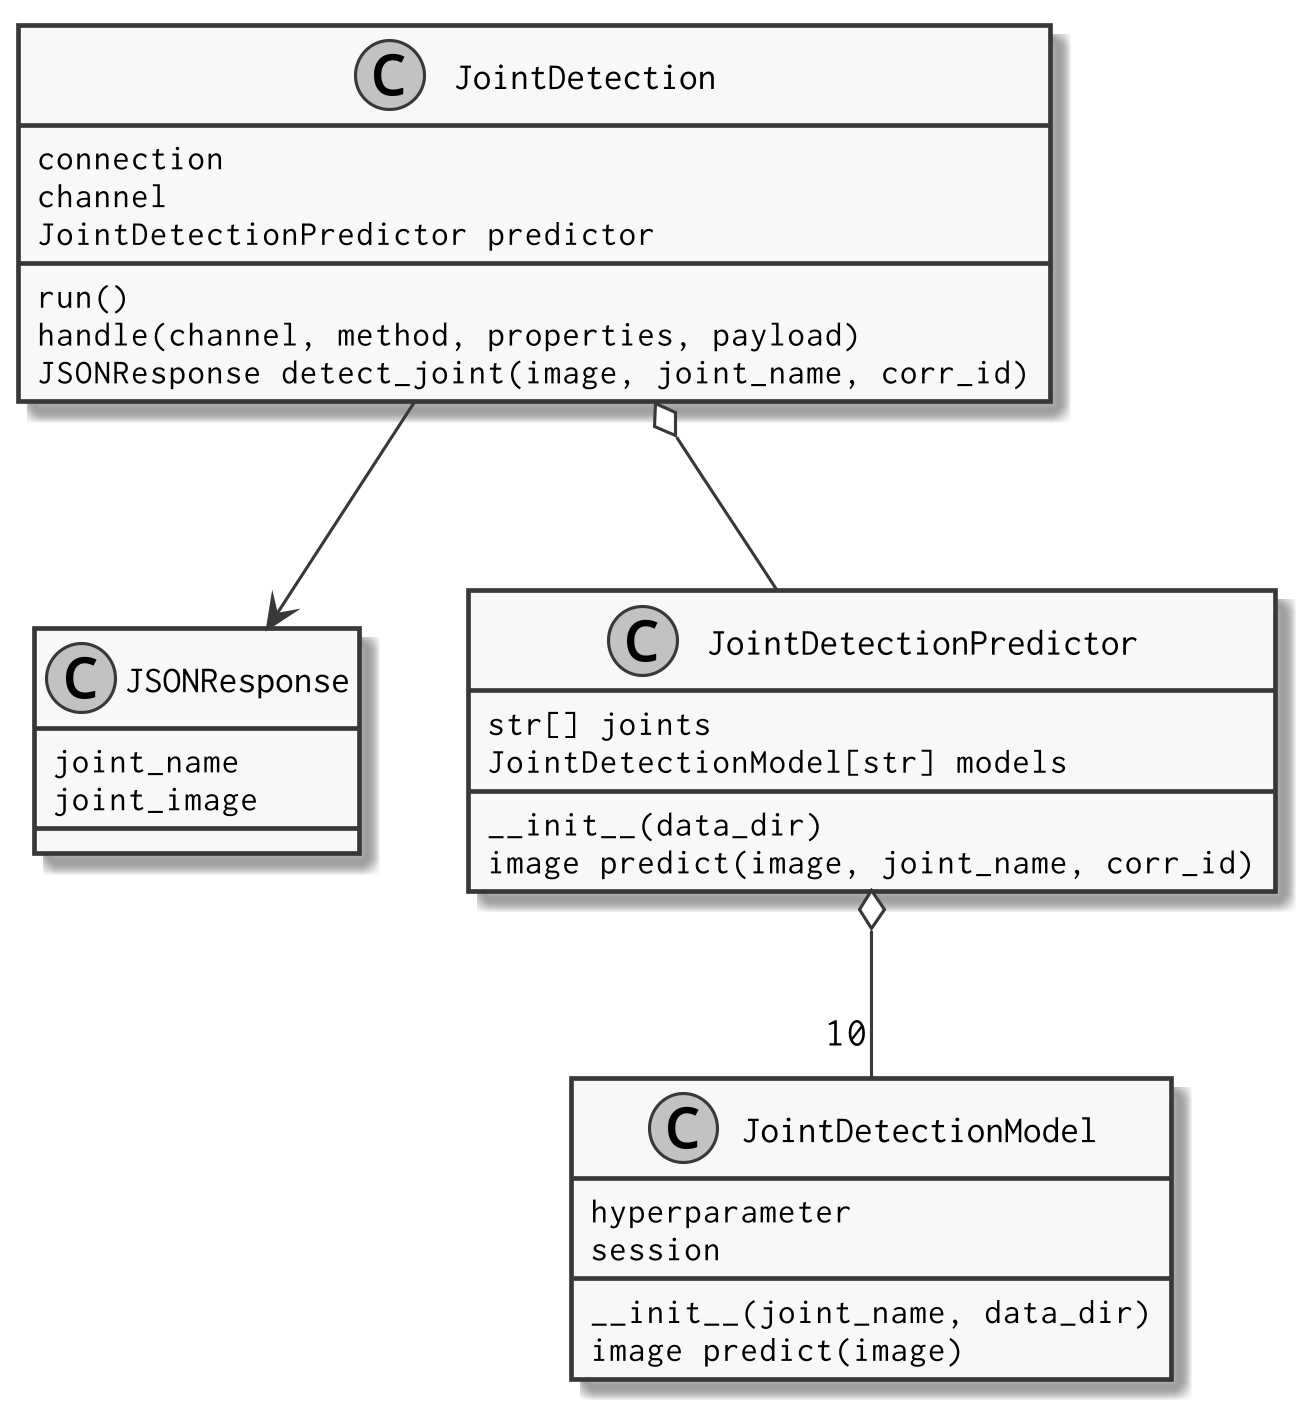
\includegraphics[width=0.9\linewidth]{pics/class-joint-detection.png}
    \caption{Die Modellkomponente \texttt{joint\_detection} verwendet zehn verschiedene Modelle und abstrahiert diese über eine zusätzliche Klasse namens \texttt{Joint\-Detection\-Model}. (Klassendiagramm)}
    \label{fig:klassendiagramm-joint-detection}
\end{figure}

Die Modellkomponente \texttt{joint\_detection} wird nicht nur einmal für alle zehn Gelenke aufgerufen (bzw. über eine entsprechende Message über die Queue \texttt{joint\_detection} angestossen), sondern einmal pro Gelenk (siehe \secref{sec:variante-4-messaging}). Darum dient als Input nicht nur ein Röntgenbild, sondern auch die Bezeichnung des zu extrahierende Gelenks. Der Payload ist eine JSON-Datenstruktur, die somit aus den Feldern \texttt{joint\_name} (Zeichenkette der Länge 4) und \texttt{xray} (base64-kodiertes JPEG-Bild) besteht.

Der Output des Modells ist wiederum ein JPEG-Bild, das base64-kodiert in der \texttt{JSONRe\-sponse} im Feld \texttt{joint\_image} abgelegt wird. Der Name des Gelenks (Feld \texttt{joint\_name}) wird auch in diese Datenstruktur eingebettet, da diese Information im nächsten Verarbeitungsschritt benötigt wird. So wird das Ergebnis nicht an den Aufrufer zurückgeliefert, sondern an die Queue \texttt{ratingen\_score} weitergeschickt. Allfällige Fehler werden in die Queue \texttt{joint\_detection\_error} geschrieben (JSON-Datenstruktur mit den Feldern \texttt{error} für die Fehlermeldung und \texttt{joint\_name} für die Gelenkbezeichnung).

Die Gelenkbezeichnung muss in jedem Fall ‒ Fehler oder Erfolg ‒ weitergegeben werden, da der \texttt{orchestrator} seinen Client erst bedienen kann, wenn er für jedes Gelenk eine Nachricht erhalten hat (siehe \secref{sec:variante-4-messaging}).

Die Klasse \texttt{JointDetectionPredictor} wird mit dem Integrationstest (\texttt{test\_joint\_de\-tect\-ion\_predictor.py}) im \texttt{tests/}-Unterverzeichnis getestet, der alle zehn Modelle für verschiedene Röntgenbilder ausführt, und prüft, ob jeweils ein Bildausschnitt zurückgeliefert wird.

\subsubsection{Modellkomponente \texttt{ratingen\_score}}

Das Scoring der Gelenke erfordert wiederum nur die Ausführung eines einzigen Machine-Learning-Modells, das mit allen zehn Gelenken gleichermassen umgehen kann. Der Parameter \texttt{joint\_name} ist für die eigentliche Prediction irrelevant, wird aber zwecks Logging trotzdem durch verschiedene Methoden gereicht. Auch im Scoring-Ergebnis (\texttt{JSON\-Re\-sponse}) muss das Gelenk vermerkt sein, damit der \texttt{orchestrator} das betreffende Gelenk beim Eintreffen der Message für den jeweiligen Vorgang als erledigt markieren kann. Die Klassesnstruktur ist auf \imgref{fig:klassendiagramm-ratingen-score} zu sehen.

\begin{figure}[tbh]
    \centering
    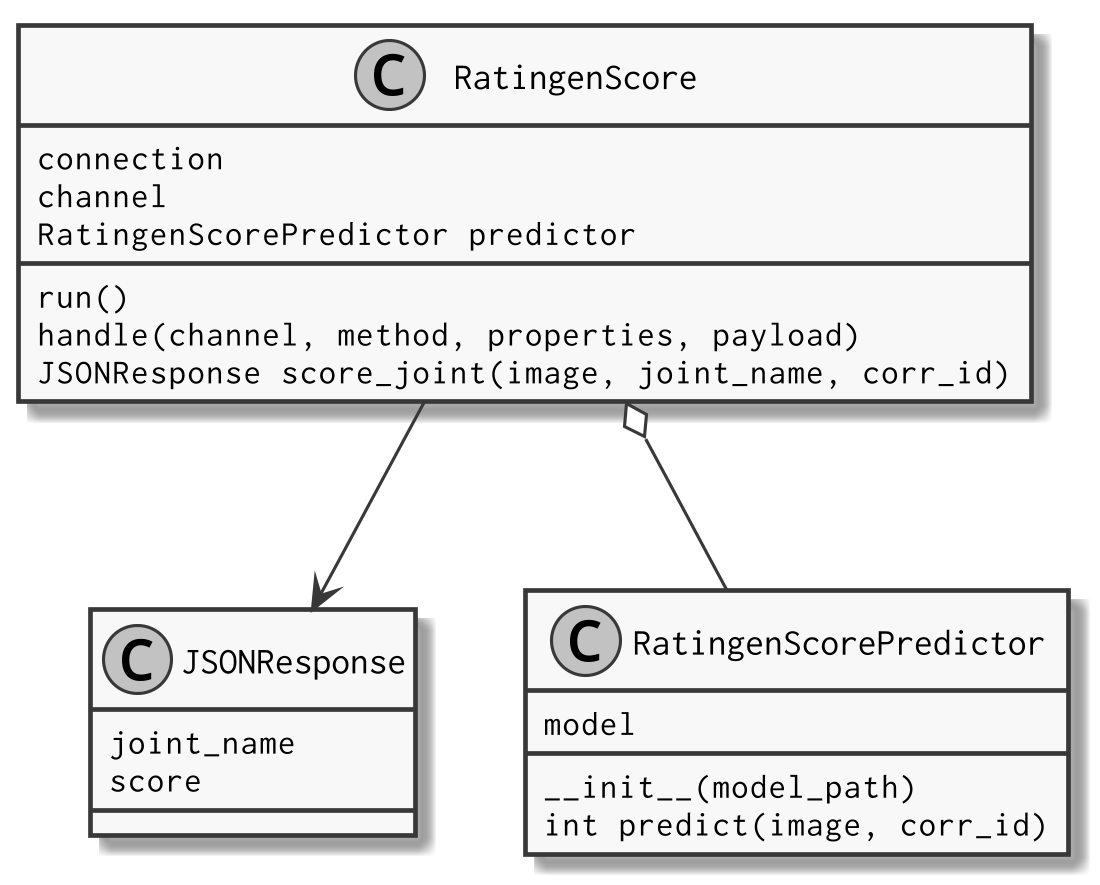
\includegraphics[width=0.9\linewidth]{pics/class-ratingen-score.png}
    \caption{Die Modellkomponente \texttt{ratingen\_score} entspricht (ähnlich wie \texttt{body\_part} in ihrer Klassenstruktur weitgehend der generischen Modellkomponente. (Klassendiagramm)}
    \label{fig:klassendiagramm-ratingen-score}
\end{figure}

Das Modell hinter dem \texttt{RatingenScorePredictor} erwartet das Bild eines Gelenks im JPEG-Format als Input, das im JSON-Payload über das Feld \texttt{joint\_image} base64-kodiert mitgegeben wird. (Das Feld \texttt{joint\_name} im JSON-Payload bezeichnet das Gelenk.) Der Output des Modells ist eine Score im Wertebereich von 0 bis 5 (siehe \secref{sec:modell-ratingen-score} zur Bedeutung dieser Scores).

Die Inputs werden von der Queue \texttt{ratingen\_score} gelesen, die Ergebnisse auf die Queue \texttt{scores} (im Erfolgsfall, mit Gelenkname und Score) bzw. \texttt{ratingen\_score\_error} (im Fehlerfall, mit Gelenkname und Fehlermeldung) geschrieben.

Die Klasse \texttt{RatingenScorePredictor} wird mit dem Integrationstest (\texttt{test\_ratingen\_score\_predictor.py}) im \texttt{tests/}-Unterverzeichnis getestet, der zehn zuvor eigenhändig ausgeschnittene Bilder von Gelenken einem Scoring unterzieht, und das Ergebnis auf Plausibilität (Wertebereich 0 bis 5) prüft.

\subsubsection{Gemeinsame technische Aspekte}
\label{sec:gemeinsame-technische-aspekte}

Die strukturellen Gemeinsamkeiten der drei Modellkomponenten wurden im Abschnitt \secref{sec:aufbau-der-modellkomponenten}  erörtert. Hier soll es nachgelagert um die \textit{technischen} Gemeinsamkeiten der erörterten Modellkomponenten gehen. Dies sind:

\begin{description}
    \item[Container] Die Modellkomponenten werden in Docker-Containern ausgeführt (siehe \secref{sec:austauschbarkeit-von-modellen}). Die Images, die jeweils im \texttt{Dockerfile} der jeweiligen Modellkomponente definiert sind, unterscheiden sich dabei voneinander. Dies hat einerseits mit den unterschiedlichen Python-Versionen (siehe \secref{sec:wahl-der-programmiersprache-modellkomponenten}), andererseits mit den komponentenspezifischen Details (Modelldaten, Abhängigkeiten der verwendeten Libraries/Frameworks in \texttt{requirements.txt} und der Code-Struktur) zu tun. Gemeinsam haben alle Images, dass sie auf einem offiziellen Python-Image basieren, die Modelldaten und den Quellcode in zwei verschiedene Verzeichnisse kopieren, alle Abhängigkeiten automatisch aus der Datei \texttt{requirements.txt} installieren, und die Hauptklasse des jeweiligen Modells ausführen.
    \item[Testing] Die verschiedenen Testfälle (Integrationstests) wurden bereits im Kontext jeder Modellkomponente kurz erläutert. Da sich die Modelle nur in einem Container ausführen lassen, müssen auch die Tests in einem Container laufen. Hierzu wird jeweils im \texttt{tests/}-Unterverzeichnis jeder Modellkomponente ein weiteres Image definiert, das auf dem Image der Modellkomponente basiert. Für dieses Image wird jeweils das Testing-Framework \texttt{pytest} installiert, der Testcode in den Container kopiert und anschliessend mit \texttt{pytest} ausgeführt. Das Erstellen des Images und Ausführen des Testcontainers erfolgt am einfachsten mit dem Shell-Skript \texttt{test.sh}, das sich im jeweiligen \texttt{tests/}-Verzeichnis befindet.
    \item[Logging] Alle Modellkomponenten geben Log-Meldungen aus. Diese enthalten jeweils den Correlation Identifier am Ende jeder Logzeile in eckigen Klammern. Es wird auf dem Level \texttt{Debug} (Meldungen zum aktuellen Verarbeitungsschritt) und \texttt{Error} (Fehlermeldungen) geloggt. Als Ausgabe dient \texttt{stdout}, und nicht wie üblich \texttt{stderr}, da bei der Ausführung mit \texttt{docker-compose} standardmässig nur Meldungen von der Standardausgabe angezeigt werden. Der Python-Interpreter wird jeweils mit dem Flag \texttt{-u} (unbuffered) gestartet, sodass Log-Meldungen unverzüglich ausgegeben und nicht in einem Puffer zwischengespeichert werden. Auch die Art der Log-Meldungen ist bei allen Modellkomponenten ähnlich, so werden folgende Ereignisse geloggt: Verbindung mit dem Message-Broker (Erfolg/Misserfolg nach \texttt{n} Versuchen), Laden des Modells (mit der dazu benötigten Zeit), Eintreffen eines Payloads (mit dessen Grösse), abgeschlossene Prediction (mit Ergebnis und dazu benötigter Zeit); und allfällige Exceptions (als Fehler). Jede Log-Meldung enthält weiter den genauen Zeitpunkt, das Log-Level und den Namen der Klasse, welche die Log-Meldung ausgegeben hat.
    \item[Verbindungsaufbau] Die Modellkomponenten sind erst voll einsatzfähig, wenn der von ihnen verwendete Message-Broker (RabbitMQ) aufgestartet ist, und sie sich mit diesem verbunden haben. Die Modellkomponenten sind somit vom Message-Broker abhängig, und ihre Container sollten idealerweise erst dann aufgestartet werden, wenn RabbitMQ bereit ist. Leider verfügt \texttt{docker-compose} über keinen Mechanismus, der diese Abhängigkeit zuverlässig abbilden könnte.\footnote{Mit \texttt{depends\_on} kann höchstens geprüft werden, ob ein Container bereits \textit{gestartet} worden ist, und nicht, ob die Container-Anwendung bereits fertig geladen und so etwa für eingehende Verbindungen \textit{bereit} ist.} Aus diesem Grund kann eine Modellkomponente nicht wissen, ob RabbitMQ schon bereit für eingehende Verbindungen ist. Eine einfache Lösung ist der wiederholte Versuch eines Verbindungsaufbaus mit einem \textit{Backoff}, wobei nach jedem gescheiterten Versuch ein bestimmtes Zeitfenster abgewartet wird, bevor ein neuer Verbindungsaufbau versucht wird. Diese Versuche werden in einem Takt von zwei Sekunden unternommen, insgesamt maximal 60 mal. Kann während dieser Zeit keine Verbindung hergestellt werden, dürfte ein Fehler im Gesamtsystem vorliegen, der vor weiteren Verbindungsversuchen zu beheben wäre.
    \item[Gemeinsamer Code] Obwohl die drei Modellkomponenten über gemeinsame Funktionalität verfügen (Verbindungsaufbau, Logging), wird zwischen ihnen keinerlei Code (zumindest kein selbstgeschriebener) geteilt. Stattdessen wurden die beiden Dateien \texttt{amqp.py} und \texttt{log.py} (zusammen ca. 50 Zeilen) für die Modellkomponenten jeweils kopiert und wenn nötig angepasst.\footnote{In \texttt{ratingen\_score} können aufgrund der Python-Version 3.5 keine f-Strings verwendet werden.} Dies mag zunächst nach einer schlechten Praxis und einem \textit{Code Smell} klingen, dürfte aber der einzige Weg sein, die \textit{unabhängige} Weiterentwicklung der Modellkomponenten zu ermöglichen. Basierten die Modellkomponenten auf einer gemeinsamen, selbstgeschriebenen Library (für Logging und Verbindungsaufbau), müsste diese für spezielle Anforderungen der Modellkomponenten jeweils angepasst und/oder erweitert werden, was die Vorwärtskompatibilität zu den anderen Modellkomponenten einschränken könnte. Zudem könnten künftige Versionen der Modellkomponenten in einer anderen Programmiersprache als Python geschrieben werden, wodurch die vormals gemeinsame Library nur noch unnötiger Ballast wäre.\footnote{Das Go-Proverb \textit{«A little copying is better than a little dependency.»} bringt zum Ausdruck, dass die Wiederverwendung von Code in manchen Fällen nicht erstrebenswert, ja gar schädlich ist \cite[9:28]{go-proverbs}.}
    \item[Legacy-Code] Die Modellkomponenten \texttt{body\_part} und \texttt{joint\_detection} ‒ sprich die beiden älteren Modelle ‒ enthalten ein \texttt{legacy/}-Verzeichnis. Dieses enthält älteren Code, der grösstenteils ohne Änderung und Reflexion von den Vorprojekten übernommen worden ist. Der Code ist funktionstüchtig, dürfte aber für die Aktualisierung der Modelle auf neuere Frameworks grössere Anpassungen erfordern, und wird im Rahmen der vorliegenden Arbeit nicht analysiert oder dokumentiert.
    \item[Modelldaten] Die Modelldaten werden beim Erstellen des Docker-Images jeweils in dieses hineinkopiert\footnote{Das Einhängen (via \texttt{mount}) über ein lokales Verzeichnis wäre schneller, würde aber die Manipulation der Modelle zur Laufzeit ermöglichen, und bietet daher eine schlechtere Isolation.}, genauer in das Verzeichnis \texttt{/usr/modeldata}.\footnote{Beim Modell \texttt{ratingen\_score} wird zusätzlich das generische Modell \textit{Inception V3} nach \texttt{/root/.keras/models} kopiert, damit die Datei nicht beim Aufstarten des Containers vom Internet heruntergeladen wird, siehe \url{https://stackoverflow.com/q/60837438/6763074} (abgerufen am 23.05.2020).} Das Verzeichnis \texttt{/usr/modeldata} wird der Python-Anwendung via Umgebungsvariable \texttt{DATADIR} zugänglich gemacht, womit die Modelldaten in die Anwendung geladen werden können.\footnote{Bei \texttt{joint\_detection} wird der Pfad zu den Modelldaten zusätzlich über den jeweiligen Gelenknamen ergänzt.}
\end{description}

\subsection{Komponente \texttt{orchestrator}}

Beim \texttt{orchestrator} handelt es sich um die zentrale Komponente des Prototyps. Der Prozess beginnt damit, dass ein Client ein Röntgenbild per HTTP an den \texttt{/score}-Endpoint (\texttt{POST}-Anfrage) sendet, der vom \texttt{orchestrator} angeboten wird, und endet damit, dass der \texttt{orchestrator} dem Client eine Reihe von Scores zurückliefert, idealerweise zehn an der Zahl. Dieser Vorgang ist in \secref{sec:variante-4-messaging} beschrieben und auf \imgref{fig:datenfluss-variante-queue-2} grafisch dargestellt.

Dieser Vorgang dauert einige Sekunden. Währenddessen sollen auch andere Clients Röntgenbilder zur Verarbeitung in Auftrag geben können, ohne auf das Ende eines laufenden Vorgangs warten zu müssen.\footnote{In der Praxis verzögern sich die einzelnen Vorgänge unter starker Last des Systems. Dieses soll aber trotzdem \textit{ansprechbar} bleiben, d.h. die Anfragen zumindest entgegennehmen und in die entsprechenden Queues zur Verarbeitung stellen.} Noch wichtiger ist, dass die Ergebnisse der beiden Vorgänge nicht durcheinandergebracht werden, sodass etwa Anfrager A, der das Röntgenbild einer gesunden Hand verarbeiten lässt, plötzlich die Score für ein geschädigtes Gelenk, das zu einem Bild von Anfrager B gehört, in seinem Ergebnis vorfinden würde.

Wie die nebenläufige Verarbeitung von Röntgenbildern korrekt und möglichst performant erfolgt, wird in Abschnitt \secref{sec:der-score-endpoint} erörtert. Zunächst soll hier aber ein Überblick über die \texttt{orchestrator}-Komponente geboten werden, der zum Verständnis des \texttt{/score}-Endpoints nötig ist.

Der \texttt{orchestrator} ist in Go (siehe \secref{sec:wahl-der-programmiersprache-orchestrator}) geschrieben, genauer in der derzeit aktuellen Version 1.14 von Go. Das \texttt{orchestrator/}-Ver\-zeich\-nis enthält die folgenden Artefakte:

\begin{description}
    \item[\texttt{Dockerfile}] Wie die Modellkomponenten läuft auch der \texttt{orchestrator} in einem Docker-Container. Aufgrund der kompilierten Natur von Go empfiehlt sich hier der Einsatz zwei verschiedener Container: einer für die Kompilierung, und einer für die Ausführung.\footnote{Im Gegensatz zu Python, das einen Interpreter zur Ausführung benötigt, kommen kompilierte Go-Programme gänzlich ohne Laufzeitumgebung aus, da die statisch gelinkten Binärdateien sämtliche Abhängigkeiten beinhalten.} Das \textit{Builder}-Image basiert auf einer aktuellen Version des Go-Docker-Images. Sämtliche Quellcodedateien, sowie die Moduldateien (\texttt{go.mod} und \texttt{go.sum}, siehe weiter unten), werden in das Image kopiert. Die Abhängigkeiten werden mit \texttt{go mod tidy} aufgelöst. Anschliessend wird das Programm kompiliert und als ausführbare Binärdatei unter \texttt{/app/orchestrator} abgelegt. Das \textit{Runtime}-Image kann diese Datei mittels \texttt{COPY --from=builder} aus dem Builder-Image herauskopieren. Der Inhalt des \texttt{cert/}-Verzeichnisses (siehe unten) wird ebenfalls in das Runtime-Image kopiert um TLS-verschlüsselte Verbindungen via HTTPS zu unterstützen. Der Port 8080 wird gegen aussen freigegeben, und \texttt{/bin/orchestrator} als Standardeinstiegspunkt definiert.
    \item[\texttt{go.mod}/\texttt{go.sum}] Bei diesen Dateien handelt es sich um die Moduldefinition. In \texttt{go.mod} werden der Name des Moduls (\texttt{code.seantis.ch/deepxray/orchestrator}), die verwendete Version von Go (1.14.2) und die verschiedenen Abhängigkeiten (\texttt{uuid} und \texttt{amqp}) definiert. In \texttt{go.sum} werden die Prüfsummen für die initial heruntergeladenen Abhängigkeiten festgehalten. Darum wird letztere Datei auch in den Build-Container kopiert, damit garantiert ist, dass immer die gleichen Abhängigkeiten verwendet werden. Weitere Details zur Verwendung von Go-Modulen finden sich im offiziellen Blog zu Go \cite{using-go-modules}.
    \item[\texttt{orchestrator.go}] Diese Datei enthält den Haupteinstiegspunkt, sprich die \texttt{main()}-Funk\-ti\-on der \texttt{orchestrator}-Komponente. Diese führt folgende Schritte aus: Zunächst wird die Verbindung mit dem Message-Broker RabbitMQ aufgenommen, wozu ein lineares Backoff verwendet wird (siehe Abschnitt \textit{Verbindungsaufbau} in \secref{sec:gemeinsame-technische-aspekte}). Als nächstes werden sämtliche Queues deklariert, die von RabbitMQ angeboten werden müssen\footnote{\tblref{tbl:schnittstellen} listet diese in der entsprechenden Spalte auf.}; auch diejenige, die nicht direkt vom \texttt{orchestrator} angesprochen wird (\texttt{ratingen\_score}). Nun wird je ein Channels auf die vier Queues geöffnet, von denen der \texttt{orchestrator} Nachrichten empfangen soll: \texttt{bodyPart\-Response} (Queue \texttt{body\_part\_response}), \texttt{jointDetectionError} (Queue \texttt{joint\_detec\-tion\_error}), \texttt{ratingenScoreError} (Queue \texttt{ratingen\_score\_er\-ror}) und \texttt{scoresRe\-sponse} (Queue \texttt{scores}). Die Handhabung dieser Channels ist weiter unten (\texttt{mes\-sag\-ing/\-mes\-sag\-ing.go}) erläutert. Schliesslich werden zwei Endpoints registriert: Erstens, der \texttt{/score}-Endpoint, der in Abschnitt \secref{sec:der-score-endpoint} erörtert wird; zweitens, ein \texttt{/canary}-Endpoint, womit geprüft werden kann, ob der Service läuft und via HTTP ansprechbar ist, und etwa zu Monitoring-Zwecken eingesetzt werden könnte. Die Endpoints werden vie TLS-Verbindung zugänglich gemacht, die über ein selbst signiertes Zertifikat verschlüsselt wird (siehe Abschnitt \texttt{cert/} weiter unten).
    \item[\texttt{httputils/httputils.go}] Dieses Untermodul enthält eine Datenstruktur \texttt{HTTPErr}, die eine Fehlermeldung (Zeichenkette) mit einem HTTP-Status-Code kombiniert. Diese kann mit der Funktion \texttt{RespondHTTPErr()} formatiert an den Client übergeben werden und schreibt die Meldung zugleich mit dem Correlation Identifier als Log-Meldung. Zwei weitere Funktionen ‒ \texttt{Respond()} und \texttt{RespondMessage()} ‒ bieten eine vergleichbare Funktionalität über eine Schnittstelle, die nicht \texttt{HTTP\-Err} verwenden, sondern atomare Werte (Status-Code als Integer, Message als Zeichenkette). Alle Funk\-ti\-onen haben gemeinsam, dass sie zu einem HTTP-Status-Code die entsprechende textuelle Beschreibung ermitteln und ausgeben. Für den Produktiveinsatz wäre zu prüfen, ob interne Fehlermeldungen dem Client vorenthalten werden sollten.
    \item[\texttt{messaging/joints.go}] Diese Datei definiert eine Map namens \texttt{BodyPartJoints}, welche einem Körperteil (\texttt{hand left}, siehe Beschreibung der \texttt{label\_map} in Abschnitt \secref{sec:modellkomponente-body-part}) den zu extrahierenden Gelenken (MCP 1-5 und PIP 1-5) zuordnet. Die Idee hinter dieser Map ist die Vorwärtskompatibilität: So soll ein erkanntes Körperteil nicht einfach statisch gegen \texttt{hand left} geprüft, sondern in \texttt{BodyPartJoints} nachgeschlagen werden. Um weitere Körperteile (und Gelenke) zu unterstützen, könnte die Map um weitere Definitionen ergänzt werden ‒ sofern die Modellkomponenten entsprechend nachgerüstet werden. Weiter ist in \texttt{joints.go} die Funktion \texttt{CreateJointDetectionRequests} definiert, die für ein Röntgenbild und eine Körperteilbezeichnung eine Reihe von \texttt{JointDetectionRequest}-Strukturen (siehe \texttt{payloads.go} weiter unten) erzeugt; eine pro Gelenk. Diese Funktion schlägt die übergebene Körperteilbezeichnung in \texttt{BodyPartJoints} nach und reagiert mit einem Fehler, falls für dieses Körperteile keine Gelenke unterstützt werden. Im Erfolgsfall werden die erstellten Strukturen als Slice zurückgeliefert.
    \item[\texttt{messaging/messaging.go}] Diese Datei enthält das Kernstück der \texttt{orchestrator}-Kom\-po\-nen\-te: die \texttt{Handle()}-Funktion, welche für die eigentliche Orchestrierung zuständig ist. Diese Funktion erwartet die vier Channels auf die Queues, die oben (siehe \texttt{orchestrator.go}) deklariert worden sind. Weiter wird hier eine Map namens \texttt{connections} verwaltet, die einem Correlation Identifier einen Channel zuordnet. Hierbei handelt es sich um den Kanal, mit dem Nachrichten aus den Queues in den Anfragekontext zurückgeleitet werden können. (Der Mechanismus wird in \secref{sec:der-score-endpoint} aus einer anderen Perspektive erläutert.) Sämtliche asynchrone Kommunikation in der \texttt{orchestrator}-Komponente läuft in dieser Funktion zusammen, genauer in einem \texttt{for/select}-Loop, der für jeden Channel einen \texttt{case}-Branch hat \cite[Kapitel 8.7]{gopl}. Neben der Channels auf die vier Message-Queues kümmert sich \texttt{Handle()} im gleichen \texttt{for/select}-Loop auch um die Registrierung und Deregistrierung von Rückkanälen, die in der \texttt{connections}-Map verwaltet werden. Ein Anfragekontext (Aufruf des \texttt{/score}-Endpoints) kann sich über den Kanal \texttt{connectChan} registrieren. Dazu sendet er eine Nachricht (\texttt{Chan\-nel\-Connection}) bestehend aus einem Correlation Identifier und einem eigens erstellten Channel an \texttt{connectChan}. (Der Kanal wird in der \texttt{connections}-Map abgelegt.) Ist der Anfragekontext am Ende seiner Lebensdauer angelangt, kann er sich über \texttt{disconnectChan} unter Angabe seines Correlation Identifiers wieder deregistrieren. (Der Kanal wird geschlossen und aus der \texttt{connections}-Map entfernt). Mithilfe dieses Konstrukts kann die Integrität der nebenläufigen Vorgänge ohne jegliche Locking-Mechanismen wie Mutexes gewährleistet werden.\footnote{Das Go-Proverb \textit{«Channels orchestrate; mutexes serialize»} bringt den Vorteil dieses Ansatzes zum Ausdruck \cite[4:21]{go-proverbs}.} Um Nachrichten aus den vier erwähnten Queues in den Anfragekontext weiterleiten zu können, wird deren Correlation Identifier verwendet. Mit diesem kann der Rückkanal in der \texttt{con\-nec\-tions}-Map nachgeschlagen werden. Der Einfachheit halber ist der Rückkanal als \texttt{byte}-Slice typisiert, sodass darüber beliebige Payloads weitergereicht werden können.\footnote{Die Art des Payloads ergibt sich dabei aus dem Kontext: So trifft die Nachricht von \texttt{body\_part} immer früher ein als diejenigen von \texttt{ratingen\_score}.} Schliesslich enthält \texttt{messaging.go} die Funktionen \texttt{DeclareQueue()} und \texttt{ConsumeQueue()}, womit die Queues mit sinnvollen Einstellungen deklariert und konsumiert werden können.\footnote{Diese Einstellungen müssten für den Produktivbetrieb noch einmal gründlich geprüft werden. Optionen wie die persistente Speicherung von Messages ergeben aber in diesem Kontext keinen Sinn, da ein HTTP-Client kaum auf einen Neustart des Systems warten würde.}
    \item[\texttt{messaging/payloads.go}] Hier sind die verschiedenen Payloads als \texttt{struct} definiert, die einerseits zwischen den Komponenten untereinander und andererseits zwischen dem \texttt{orchestrator} und dem Client ausgetauscht werden. Diese entsprechen weitgehend den Strukturen, die in \tblref{tbl:schnittstellen} aufgelistet sind. Eine Ausnahme bildet die Struktur \texttt{ScoreResponse}, die sowohl für Fehlermeldungen als auch für Scoring-Ergebnisse verwendet werden kann, indem sie die Felder \texttt{score} \textit{und} \texttt{error} enthält. Der Marshaling-Mechanismus von Go füllt dabei einfach die Felder ab, die im Payload zu finden sind, und lässt das jeweils andere Feld leer. Die Entscheidung, ob es sich bei der Datenstruktur eine Fehlermeldung oder um ein Scoring-Ergebnis handelt, ist der Interpretation des Aufrufers überlassen. Die einzelnen Felder der Strukturen sind zwecks Marshaling mit \texttt{json}-Tags annotiert \cite[Kapitel 4.5]{gopl}.
    \item[\texttt{cert/}] Dieses Verzeichnis enthält ein selbst signiertes TLS-Zertifikat, womit die Verbindung zwischen dem \texttt{orchestrator} und dem HTTP-Client verschlüsselt wird. Da der Prototyp zu Test- und Demozwecken auf einem Cloud-Server ausgeführt werden soll, und diesem echte, d.h. schützenswerte Röntgenbilder übertragen werden, ist dieser einfache Schutzmechanismus angebracht, wenn auch für die Praxis untauglich.\footnote{HTTP-Clients wie \texttt{curl} benötigen einen zusätzlichen Parameter, damit ein nicht verifiziertes TLS-Zertifikat für den Verbindungsaufbau akzeptiert wird.} Das \texttt{Makefile} im Verzeichnis dient dazu, ein neues Zertifikat über den Befehl \texttt{make} zu erstellen. Der Aufruf von \texttt{openssl} mit all den benötigten Parametern wird dadurch vereinfacht. Das Zertifikat wird beim Erstellen des Docker-Images in diesen integriert, und beim Aufstarten vom \texttt{orchestrator} geladen.
\end{description}

\subsubsection{Der \texttt{/score}-Endpoint}
\label{sec:der-score-endpoint}

Der Überblick über den \texttt{orchestrator} aus dem vorherigen Abschnitt sollte einen Rahmen schaffen, um die Rolle des \texttt{/score}-Endpoints besser verständlich zu machen. Dieser wird in der Funktion \texttt{createScoringEndpoint} als Closure \cite[S. 136]{gopl} erzeugt und zurückgegeben.\footnote{HTTP-Endpoints werden in Go als Funktionen gehandhabt, die dem Interface \texttt{http.Handler} genügen \cite[Kapitel 7.7]{gopl}.} Diese Closure benötigt als Kontext den AMQP-Channel (\texttt{amqpChan}), die Queue zum Zugriff auf die Antworten von \texttt{body\_part} (\texttt{bodyPartResponse\-Queue}) und die beiden Channels zum Registrieren und Deregistrieren des Rückkanals mit einem Correlation Identifier (\texttt{connectChan} und \texttt{disconnectChan}).

Die Funktionsweise des \texttt{/score}-Endpunkts lässt sich am besten sequenziell erläutern:

\begin{enumerate}
    \item Der Client ruft den Endpoint via HTTP (\texttt{POST}-Methode) auf. Wird eine andere Methode verwendet, erhält der Client als Antwort Status 405 (Method not Allowed) und der Vorgang wird abgebrochen.
    \item Der Payload (JPEG-Röntgenbild als Form File \texttt{xray}) wird in der Funktion \texttt{loadXRay} ausgelesen. Fehlt dieser, erhält der Client als Antwort Status 400 (Bad Request); der Vorgang wird abgebrochen. Ist er vorhanden, wird das Bild in einen Puffer gelesen und zurückgegeben.
    \item Es wird ein Correlation Identifier (eine zufällige UUID) erzeugt.\footnote{\url{https://godoc.org/github.com/google/uuid\#NewRandom} (abgerufen am 24.05.2020)} Sollte dies fehlschlagen, erhält der Client Status 500 (Internal Server Error) als Antwort.
    \item Der Rückkanal wird als Channel vom Typ \texttt{[]byte} erzeugt und mit dem Correlation Identifier zusammen in einer \texttt{messaging.ChannelConnection} an den \texttt{connectChan} gesendet, um diesen zu registrieren. In einem \textit{deferred call}, der unmittelbar danach definiert ist, wird der Correlation Identifier an den \texttt{disconnectChan} gesendet. Dadurch wird der Kanal in jedem Fall deregistriert (und geschlossen), egal über welchen Pfad die Funktion des \texttt{/score}-Endpoints verlassen wird \cite[S. 145]{gopl}.
    \item Das Röntgenbild wird mit der Funktion \texttt{publishToBodyPart} in die Queue \texttt{body\_part} gestellt. Sollte dies scheitern, wird dem Client Status 500 (Internal Server Error) zurückgeliefert. Andernfalls sollte nun die Erkennung des Körperteils angestossen worden sein.
    \item Die Antwort von \texttt{body\_part} wird synchron vom Rückkanal (\texttt{ch}) abgewartet. Trifft sie ein, wird sie in der Funktion \texttt{processBodyPartResponse} verarbeitet, indem die Bytes in die entsprechende JSON-Struktur umgewandelt werden (Unmarshaling). Ein Fehler würde wiederum mit Status 500 (Internal Server Error) an den Client geschickt.
    \item Für das erkannte Körperteil werden mit \texttt{createJointDetectionRequests} die Nachrichten für die Gelenkextraktion erzeugt. Wie weiter oben für \texttt{joints.go} beschrieben worden ist, findet hier keine explizite Prüfung auf das Körperteil statt. Sollte es für das Körperteil keine extrahierbaren Gelenke geben, wird Status 501 (Not Implemented) an den Client zurückgeliefert, da das jeweilige Körperteil nicht zur Verarbeitung unterstützt wird. Wurde eine linke Hand auf dem Röntgenbild erkannt, werden zehn Messages für die Gelenkextraktion erzeugt und (mit \texttt{toJSON}) in JSON umgewandelt. Das Röntgenbild wird hierzu base64-kodiert.
    \item Die (zehn) Messages zur Extraktion werden mit \texttt{sendJointDetectionPayloads} auf der Queue \texttt{joint\_detection} publiziert.
    \item Der Payload für die Antwort an den Client wird initialisiert. Dieser enthält eine Map von Scores (\texttt{string} zu \texttt{int}). Nun beginnt das Warten auf die eintreffenden Nachrichten (Fehlermeldungen oder ermittelte Scoring-Ergebnisse).
    \item Bis zu diesem Punkt dürfte der Client weniger als eine Sekunde gewartet haben. Bis alle Ergebnisse beim \texttt{orchestrator} eingetroffen sind, und diese an den Client weitergerreicht werden können, dürften nun einige Sekunden vergehen.\footnote{Benchmarks auf einem aktuellen Laptop und auf einem Cloud-Server (auf Arch bzw. Debian Linux) zeigen, dass der Client sich ca. acht bis zwölf Sekunden gedulden muss, bis er eine Antwort bekommt.} Bei hoher Last erhöht sich die Wartedauer. Diese soll limitiert werden, indem ein festes Timeout von 60 Sekunden definiert wird. Hierzu wird eine \textit{goroutine} gestartet, die 60 Sekunden abwartet und dann über einen Channel meldet, dass sie abgelaufen ist.
    \item Nun wird in einem Loop auf die eintreffenden Antworten gewartet (eine Iteration pro Gelenk). Hierzu dient ein \texttt{select}-Statement, das zwei \texttt{case}-Branches hat: Einerseits für die Ergebnisse aus dem Rückkanal (Channel \texttt{ch}), andererseits vom vorher beschriebenen Timeout-Kanal. Trifft eine Meldung über \texttt{ch} ein, wird diese ausgewertet (Fehlermeldung oder Score) und dem Payload für die Client-Response hinzugefügt. Läuft in diesem Loop das Timeout ab, und wird dies über den entsprechenden Kanal gemeldet, erhält der Client den Status 408 (Request Timeout) \textit{ohne} partiellen Payload gemeldet. Der Vorgang wird damit abgebrochen.
    \item Konnten hingegen alle (zehn) Antworten «eingesammelt» werden, ohne dass in der Zwischenzeit das Timeout abgelaufen ist, wird der Payload als JSON an den Client gesendet (Status: 200 OK) und geloggt.
\end{enumerate}

Der Vorgang ist hiermit abgeschlossen. (Der Rückkanal wird, wie oben erwähnt, über einen \textit{deferred call} deregistriert und geschlossen.) Während dieses Vorgangs können andere Anfragen auf den \texttt{/score}-Endpoint abgesetzt werden. Diese werden jeweils in einem gesonderten Funktionskontext abgearbeitet und haben ihren eigenen Correlation Identifier. Die verschiedenen Vorgänge kommen sich also nicht in die Quere.

\subsubsection{Testen des \texttt{/score}-Endpoints}

Wie bereits in der Teststrategie skizziert (siehe \secref{sec:teststrategie}), kann der \texttt{/score}-Endpoint bedeutend effektiver von einem Systemtest (End-to-End) als von einer Reihe von Unit- oder Integrationstests abgedeckt werden. Im \texttt{test/}-Verzeichnis befinden sich mehrere Varianten dafür:

\begin{description}
    \item[\texttt{test.sh}] Hierbei handelt es sich um ein einfaches Bash-Skript, das den \texttt{/score}-Endpoint mit vier verschiedenen Röntgenbildern aufruft. Diese zeigen: je eine geschädigte Hand (\texttt{bad1.jpg} und \texttt{bad2.jpg}), eine gesunde Hand (\texttt{good.jpg}) und einen Fuss (\texttt{foot\-.jpg}). Für die drei Aufrufe mit einer linken Hand wird der zurückgelieferte Payload mit \texttt{jq} formatiert und in JSON-Dateien abgelegt. Dieses Testskript nimmt keine weiteren Auswertungen vor und diente vorallem während der Entwicklung zum Testen.
    \item[\texttt{test.py}] Dies ist ein Python-Skript, das mithilfe der \texttt{requests}-Library die gleichen Bilder verarbeiten lässt wie das zuvor genannte Bash-Skript. Im Gegensatz dazu wird hier auch der Status-Code der Antwort geprüft (200 bei den Händen, 501 beim Fuss). Das Skript diente dazu, die \texttt{requests}-Library auszuprobieren, die bei der systematischen Evaluation (siehe \secref{sec:technische-evaluation}) zum Einsatz kam.
    \item[\texttt{deepxray\_test.go}] Dieser Testfall wurde in Go geschrieben und ist der mächtigste der dreien. Die Testfälle sind in einer Map namens \texttt{tests} abgelegt und folgen dem Paradigma des \textit{table-driven test design} \cite[S. 306]{gopl}. Als Key dient jeweils der Dateiname eines Röntgenbildes; als Value wird eine Struktur verwendet, die einerseits den erwarteten HTTP-Status-Code (200 oder 501), und andererseits eine Map von erwarteten Scores (\texttt{"pip1": 0, "pip2": 1}, usw.) enthält. Die Testfunktion \texttt{TestScoringAsync} führt diese Testfälle \textit{asynchron} aus, d.h. startet für jeden Testfall eine eigene \textit{goroutine}. Mithilfe einer \texttt{WaitGroup} \cite[S. 238]{gopl} wird darauf gewartet, dass alle gesendeten Requests beantwortet worden sind. Die Auswertung der Antworten, d.h. der Vergleich zwischen den erwarteten und den eingetroffenen Scores, wird dabei in jeder Request-\textit{goroutine} durchgefürt. So kann geprüft werden, dass bei mehreren nebenläufigen Vorgängen keine Scores durcheinandergeraten. Weiter enthält diese Datei einen Benchmark, der die gleiche Datei (\texttt{bad2.jpeg}) zehnmal an den \texttt{/score}-Endpoint schickt und anschliessend die durchschnittliche Verarbeitungszeit misst. Der Test kann mit \texttt{go test}, der Benchmark (inkl. Test) mit \texttt{go test -bench=.} gestartet werden.
\end{description}

\subsection{Web-Oberfläche}

Um den Prototyp anschaulich demonstrieren zu können, wurde im Verzeichnis \texttt{gui/} eine kleine Web-Oberfläche entwickelt. Diese wurde in Go umgesetzt und rendert das HTML serverseitig \cite[Kapitel 4.6]{gopl}. Die Anwendung wird analog zum \texttt{orchestrator} in einem Docker-Image kompiliert und in einem zweiten ausgeführt. Die Anwendung ist über Port 8888 via HTTPS erreichbar.

Der Benutzer kann ein Röntgenbild hochladen und mit Betätigung der Schaltfläche \textit{Score} zur Verarbeitung abschicken. Nach einigen Sekunden erscheint links das hochgeladene Röntgenbild. In der mittleren Spalte werden die Scoring-Ergebnisse mit einem entsprechenden Farbcode\footnote{von grün wie gesund, über gelb wie mittelstark geschädigt, bis rot wie stark geschädigt} angezeigt. Rechts ist ein Röntgenbild mit markierten Gelenken als Legende dargestellt, damit der Benutzer Bezeichnungen wie \textit{MCP 1} oder \textit{PIP 3} einfacher dem hochgeladenen und links angezeigten Röntgenbild zuordnen kann.\footnote{Die Gelenke direkt mit farbigen Quadraten auf dem Originalbild zu markieren, wäre ein schönes Feature, das jedoch eine umfassende Erweiterung des Prototyps erfordern würde (siehe \secref{sec:weitere-ideen}).}

Auf die Funktionsweise der Web-Oberfläche soll hier nicht weiter eingegangen werden, da diese nur ein Nebenprodukt des Projekts ist.

Die Web-Oberfläche ist auf \imgref{fig:webgui} zu sehen.

\begin{figure}[tbh]
    \centering
    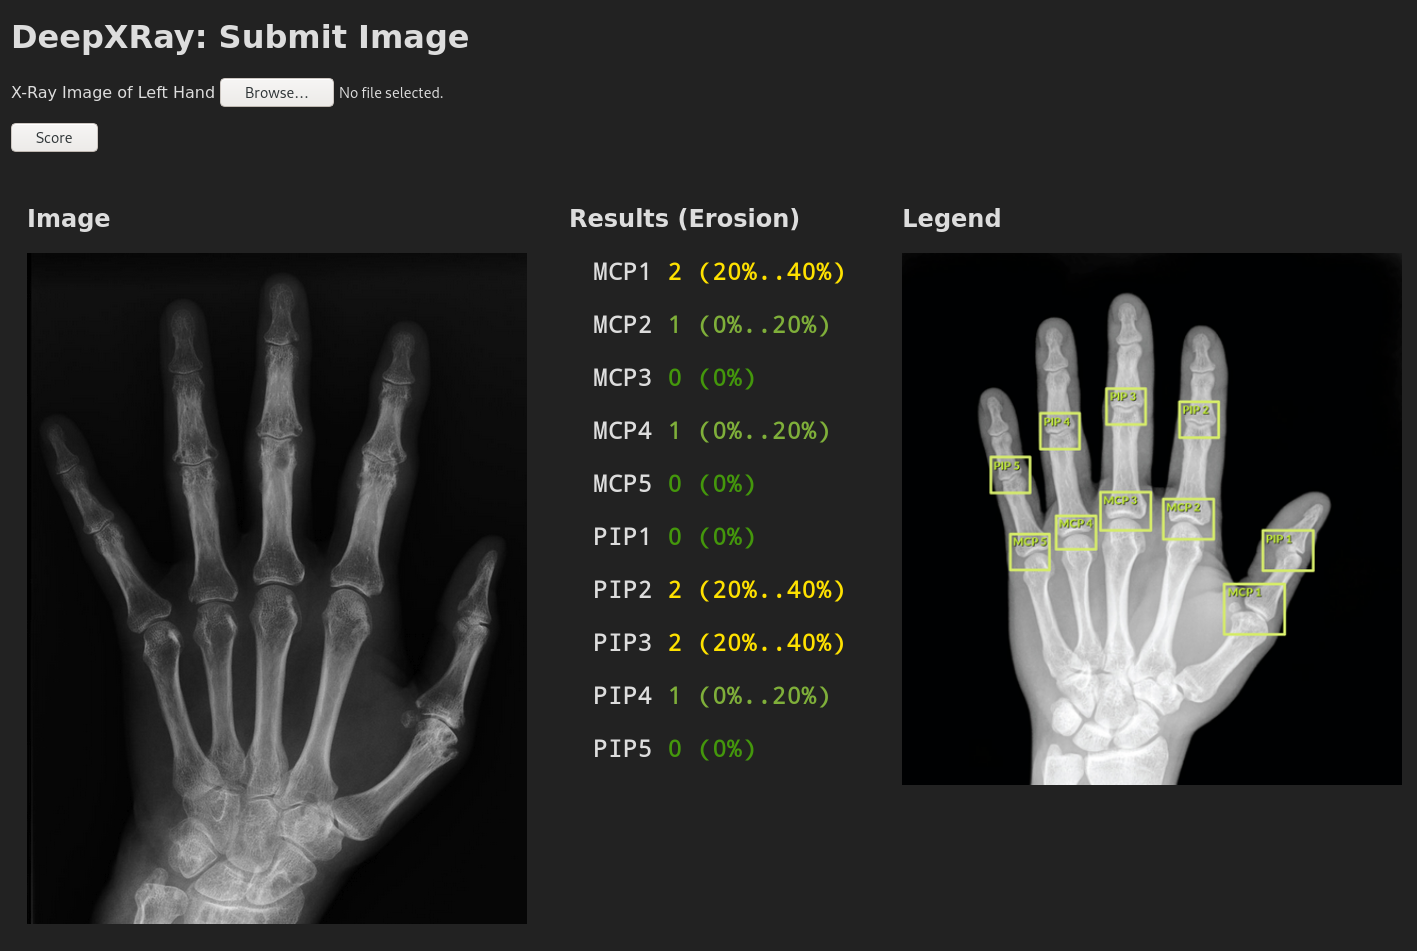
\includegraphics[width=\linewidth]{pics/web-ui-demo.png}
    \caption{Die Web-Oberfläche, auf der links das verarbeitete Röntgenbild (\textit{Case courtesy of Assoc Prof Frank Gaillard, Radiopaedia.org, rID: 3031}), in der Mitte die Scoring-Ergebnisse und rechts eine Legende mit beschrifteten Gelenken zu sehen sind. Die Schädigungen der Gelenke bewegen sich im tiefen bis mittleren Bereich.}
    \label{fig:webgui}
\end{figure}

\clearpage

\newpage

\section{Evaluation}

In diesem Kapitel geht es um die Evaluation der Arbeit. Dies ist im doppelten Sinne zu verstehen: Einerseits soll der erstellte Prototyp anhand verschiedener Metrtiken (siehe \secref{sec:evaluationsmetriken}) evaluiert werden (technische Evaluation); andererseits soll das Ergebnis der Arbeit in einem übergeordneten Kontext, der auch den vorliegenden Bericht umfasst, im Bezug auf die Zielerreichung (siehe \secref{sec:projektauftrag}) evaluiert und reflektiert werden (Evaluation des Zielerreichung).

\subsection{Technische Evaluation}
\label{sec:technische-evaluation}

Der erstellte Protoyp kombiniert drei bestehende Modelle bzw. drei Arten von Modellen zu einem Gesamtsystem, das gegen aussen den Eindruck erweckt, als würde nur eine Art von Prediction erstellt: das Scoring der Gelenke. Das Erkennen des Körperteils und die Extraktion der Bildausschnitte, welche die Gelenke zeigen, ist für den Endanwender transparent.

Für die einzelnen Modelle (\texttt{body\_part}, \texttt{joint\_detection} und \texttt{ratingen\_score}) gibt es teilweise bereits Evaluationsmechanismen. Diese wurden im Rahmen der Entwicklung der einzelnen Modelle erstellt. Soll ein einzelnes Modell verbessert werden, ist dieses isoliert im Rahmen dieses Vorgangs zu evaluieren.

Im Rahmen der vorliegenden Arbeit soll es nur um die Evaluation des Gesamtsystems gehen. Wird ein bestehendes Modell verbessert, hat dies Einfluss auf die Performance des Gesamtsystems. Diese Verbesserung soll mit einem Evaluationsworkflow ermittelt werden können. Dieser kann dabei behilflich sein, den Fokus für die Verbesserung bestehender Modelle richtig zu legen, sodass man Aufwand in diejenigen Modelle steckt, deren Verbesserung einen Performancegewinn für das Gesamtsystem bedeuten.\footnote{Mit \textit{Performance} ist in diesem Kontext v.a. die Qualität der Predictions gemeint. Betreffend Laufzeitperformance wären Verbesserungen am Modell \texttt{joint\_detection} jedoch auch sehr wünschenswert.}

Da die Modelle im laufenden Betrieb nicht weitertrainiert werden, bietet sich eine \textit{Off\-line-Evaluation} an. Für die Offline-Evaluation eines Modells (bzw. eines Systems von Modellen) gibt es verschiedene Varianten: \textit{Hold-Out Validation}, \textit{Cross-Validation}, \textit{Bootstrapping} \cite[S. 19]{zheng2015}. Die Hold-Out Validation ist eine einfache Variante, erfordert aber ein zusätzliches Evaluationsdatenset, das einerseits unabhängig von und andererseits gleich verteilt wie das Trainingsdatenset sein muss (i.i.d.: \textit{independently and identically distributed}).\footnote{Ob die \textit{i.i.d.}-Hypothese für das Test- und das Evaluationsdatenset zutrifft, soll nicht im Rahmen der vorliegenden Arbeit geprüft werden. Die Problematik wird in \secref{sec:ungeloeste-probleme} erläutert.}

\subsubsection{Evaluationsdaten}
\label{sec:evaluationsdaten}

Als Quelle für die Trainingsdaten aller involvierter Modelle diente die SCQM-Datenbank. Für das Trainieren der Modelle wurden umfassende Datensätze daraus verwendet. In der Zwischenzeit ist die SCQM-Datenbank weiter angewachsen, sodass es eine signifikante ‒ und wichtiger: stetig wachsende ‒ Anzahl neuer Testdaten gibt, die zum Zeitpunkt der Erstellung der Modelle noch nicht vorhanden waren. Da die Modelle auf das Jahr 2018 (und früher) zurückgehen, können die Daten ab dem 1. Januar 2019 für die Evaluation verwendet werden. Diese wurden noch von keinem der drei Modelle «gesehen».

Für die Auswahl der Evaluationsdaten wurden vom Auftraggeber zwei CSV-Dateien zur Verfügung gestellt\footnote{Diese Dateien befinden sich aus Gründen des Datenschutzes nicht im Abgabeordner.}: Die eine enthält u.a. die eigentlichen Scores mit Datumsangaben und Referenzen auf die zugrundeliegende Studie. Die andere erhält Informationen zu den Studien, u.a. auch die Referenz auf den Patienten. Die Informationen aus den beiden Dateien müssen kombiniert werden\footnote{Dies wurde mit dem Python-Skript \texttt{deepxray/test\_data\_selection/extract.py} bewerkstelligt}, um so die Dateinamen ableiten zu können. Aufgrund dieser Selektion konnten vom Auftraggeber 1619 Röntgenbilder zur Verfügung gestellt werden, die jedoch verschiedene Körperteile zeigen.

Es musste somit eine Selektion vorgenommen werden, sodass im Evaluationsdatenset nur Röntgenbilder linker Hände zu finden sind. Anhand der Metadaten (erwähnte CSV-Dateien) ist dies leider nicht möglich. Eine Selektion anhand der Scores (mindestens eine Score von MCP1-5 oder PIP1-5 ungleich null) ist auch nicht möglich, da die SCQM-Datenbank auch Bilder gesunder Hände enthält. Die Selektion hatte darum manuell zu erfolgen. Um den mechanischen Vorgang der Kategorisierung von 1619 Röntgenbildern ‒ zeigt es eine linke Hand oder ein anderes Körperteil? ‒ komfortabler vornehmen zu können, wurde ein Python-Skript geschrieben, womit sich die Bilder interaktiv kategorisieren lassen.\footnote{Siehe \texttt{deepxray/test\_data\_selection/categorize.py}. Das Skript arbeitet die CSV-Datei ab, die alle Scores und Dateinamen enthält. Jedes Bild wird in Firefox in einem neuen Tab geöffnet. Dabei wandert der Fokus \textit{nicht} auf ein anderes Fenster, sondern bleibt auf der Kommandozeile. Zeigt das Bild eine linke Hand, kann \texttt{a} (wie «accept») und \texttt{[Return]} eingegeben werden, um die Zeile aus der CSV-Datei sowie das Bild zu übernehmen. Gibt man nur \texttt{[Return]} ein, werden Bild und CSV-Zeile verworfen.} Auf diese Weise konnten von den ursprünglichen 1619 Röntgenbildern 290 Aufnahmen linker Hände selektiert werden.

Die CSV-Dateien enthalten zu jedem Bild die Scores aller relevanter Gelenke (MCP 1-5, PIP 1-5). Diese Scores liegen in Prozentangaben vor. Da der Prototyp, bzw. das zugrundeliegende Modell \texttt{ratingen\_score} nur mit sechs Klassen umgehen kann, müssen diese Prozentangaben in Scores umgerechnet werden.\footnote{Dies wird mit dem Python-Skript \texttt{deepxray/test\_data/extract\_information.py} bewerkstelligt. Dieses Skript übernimmt nur eine Teilmenge der Informationen aus der urpsrünglichen CSV-Datei, sodass diese als \texttt{deepxray/test\_data/part.csv} zur Verfügung gestellt werden kann.} Das Evaluationsdatenset steht nun zum Scoring bereit.

\subsubsection{Scoring der Evaluationsdaten}

Die Daten und Python-Skripts zum Vornehmen des Scorings und Auswerten der Ergebnisse (die eigentliche Evaluation) befinden sind im Abgabeordner im Unterverzeichnis \texttt{deepxray/evaluation/}. Das Scoring der Röntgenbilder erfolgt mit einem Python-Skript, das den Prototyp mithilfe der \texttt{requests}-Library anspricht.\footnote{Siehe \texttt{deepxray/evaluation/scoring/scoring.py}. Zum Zeitpunkt des Scorings wurde noch HTTP ohne TLS verwendet.} Von den ursprünglich 290 Röntgenbildern konnten in ca. 55 Minuten 247 verarbeitet werden. Auf 42 Bildern wurde fälschlicherweise keine linke Hand erkannt, worauf der Vorgang abgebrochen worden ist (HTTP-Status 501: Not Implemented).\footnote{Aufgrund der Testdatenselektion, die nur linke Hände zum Ergebnis hatte, kann es nur \textit{false negatives} (linke Hand nicht als solche erkannt) und keine \textit{false positives} (anderes Körperteil als linke Hand erkannt) geben.} Ein weiteres Bild konnte aus bisher unbekannten Gründen nicht verarbeitet werden.\footnote{In der Logdatei \texttt{deepxray/evaluation/scoring/scoring.log} lassen sich hierfür keine Hinweise finden.}

Die Bilder, für die keine maschinelle Prediction erstellt werden konnte, werden für den weiteren Evaluationsworkflow nicht berücksichtigt.\footnote{Die CSV-Datei \texttt{deepxray/evaluation/scoring/results.csv}, welche die Resultate enthält, umfasst darum nur 247 Datensätze.} Als Erkenntnis ist aber hier festzuhalten, dass \texttt{body\_part} $\frac{42}{290}=0.145$, d.h. fast 15\% \textit{false negatives} produzierte. Die folgenden weiteren Evaluationsmetriken sind daher in erster Linie von der Performance der Modelle \texttt{joint\_detection} und \texttt{ratingen\_score} abhängig.

\subsubsection{Wahl der Evaluationsmetriken}

In \secref{sec:evaluationsmetriken} wurden verschiedene Evaluationsmetriken vorgestellt und auf ihre Eignung für das vorliegende Problem (Bewertung von Röntgenbildern) geprüft. Von den vorgestellten Metriken sind folgende umgesetzt worden\footnote{Siehe das Python-Modul \texttt{evaluation} im Verzeichnis \texttt{deepxray/evaluation/evaluation} [sic.] für deren Implementierung. Als Ergänzung zur Teststrategie (\secref{sec:teststrategie}) ist anzumerken, dass der Code für die Metriken umfassend mit Unittests (\texttt{pytest}-Framework) getestet worden ist. Diese können mit \texttt{make test} ausgefürt und mit \texttt{make cover} zusätzlich auf die Codeabdeckung geprüft werden (Requirements: \texttt{pytest} und \texttt{pycover}).}:

\begin{multicols}{2}
    \begin{enumerate}
        \item Global Accuracy
        \item Class Accuracy
        \item Precision
        \item Recall
        \item F1-Score
        \item Cohen's Kappa
        \item Cohen's Quadratic Kappa
    \end{enumerate}
\end{multicols}

Der Goldstandard für das vorliegende Problem wäre wohl die \textit{Interclass Correlation}, abgekürzt ICC \cite[Abschnitt 3.3, S. 5-6]{rohrbach2019}. Da für die Evaluation jedoch nur die Einschätzungen eines Scorers pro Datenpunkt (Gelenk) verfügbar ist (siehe \secref{sec:evaluationsdaten}), kann diese Evaluationsmetrik hier nicht angewendet werden.

\subsubsection{Umsetzung der Evaluationsmetriken}

Beim Modell \texttt{ratingen\_score}, das den sichtbaren Output des Gesamtsystems ausmacht, bzw. beim weiterentwickelten Modell, das in der vorliegenden Arbeit nicht zur Verfügung steht, wurde bemerkt, dass die Übereinstimmung zwischen menschlichem Scorer und maschineller Prediction mit 47.5\% auf den ersten Blick eher bescheiden ausfällt. Erlaubt man jedoch die Abweichung von einer Klasse nach oben und nach unten, liegt die Übereinstimmung bei beträchtlichen 83\%. Aus diesem Grund sollen die aufgelisteten Metriken in zwei Ausprägungen berechnet werden: Einerseits basierend auf einem «harten» Vergleich (keine Abweichungen erlaubt), andererseits basierend auf einem \textit{«Soft Match»}, d.h. Abweichungen von ±1 werden als Übereinstimmung gewertet. So kann ein ausgewogeneres Gesamtbild der Performance geliefert werden.\footnote{In der Praxis kann es durchaus einen Unterschied machen, ob eine Einschätzung nur leicht oder um einen grossen Betrag danebenliegt.}

Die gewählten Evaluationsmetriken basieren grösstenteils auf einer Konfusionsmatrix (\textit{Confusion Matrix}). Diese listet auf der x-Achse die menschlich ermittelten Scores (\textit{Actual}) und auf der y-Achse die maschinell ermittelten Scores (\textit{Prediction}) auf. Die «harte» Konfusionsmatrix, die auf exakten Übereinstimmungen basiert, wird mit der Funktion \texttt{create\_confusion\_matrix} erzeugt.\footnote{Siehe \texttt{deepxray/evaluation/evaluation/matrix.py}.} Für die Soft Matches wird eine «weiche» Konfusionsmatrix mit der Funktion \texttt{create\_confusion\_matrix} gemäss folgender Logik erzeugt:

\begin{enumerate}
    \item Es wird ein NumPy-Array aus Nullen mit der Dimension 6x6 (Matrix) erzeugt.
    \item Es wird über eine Liste iteriert, bei welcher jedes Gelenk durch eine Tupel bestehend aus zwei Werten ‒ menschlich ermittelte Score (\textit{actual}) und maschinell ermittelte Score (\textit{prediction}) ‒ repräsentiert ist.\footnote{Die Daten kommen über die Funktion \texttt{extract\_human\_machine\_results()} aus der CSV-Datei \texttt{deepxray/evaluation/scoring/results.csv}.}
    \item Fehlt für ein Gelenk eine Score (\textit{actual} oder \textit{prediction}), wird der Eintrag ignoriert und taucht nicht in der Matrix auf.
    \item Die menschlich ermittelte Score wird als Referenz genommen. Weicht die maschinell ermittelte Score maximal um den Betrag von 1 ab, wird die maschinelle Score auf diesen Wert angepasst. Fällt die Abweichung grösser aus, wird die maschinelle Score beibehalten.
    \item Die Matrix wird an der entsprechenden Koordinate (Zeile der maschinellen, Spalte der menschlich ermittelten Score) um den Wert 1 erhöht.
\end{enumerate}

Diese Konfusionsmatrizen enthalten jeweils absolute Werte, d.h. jedes Feld repräsentiert eine Anzahl von Gelenken. Summiert man die Werte der Matrix auf, und teilt den Wert jedes Feldes durch diese Summe, erhält man eine normalisierte Konfusionsmatrix. Die vier Kombinationen aus exakt/soft und absolut/normalisiert sind auf \imgref{fig:konfusionsmatrizen} zu sehen.\footnote{In \texttt{deepxray/evaluation/evaluation/visualizations.py} kann nachvollzogen werden, wie aus den NumPy-Matrizen Grafiken erstellt worden sind. Weiter wird ein Histogramm erzeugt, das jedoch nur wenig aussagekräftig ist.}

\begin{figure}[tbh]
    \centering
    \begin{subfigure}{0.45\textwidth}
        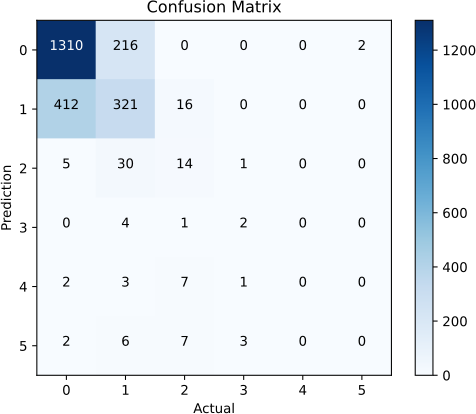
\includegraphics[width=\linewidth]{pics/confusion_matrix.png}
        \caption{Die exakte Konfusionsmatrix mit absoluten werten (Anzahl Gelenke).}
    \end{subfigure}
    \hfill
    \begin{subfigure}{0.45\textwidth}
        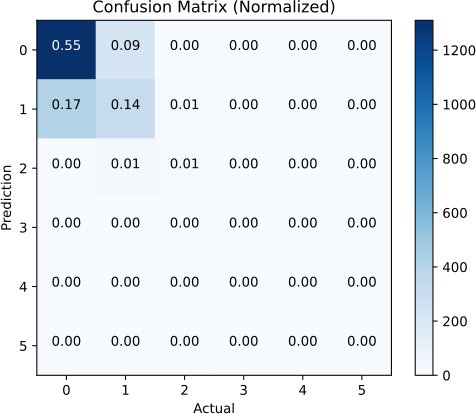
\includegraphics[width=\linewidth]{pics/confusion_matrix_norm.png}
        \caption{Die exakte Konfusionsmatrix normalisiert.}
    \end{subfigure}
    \par\bigskip
    \begin{subfigure}{0.45\textwidth}
        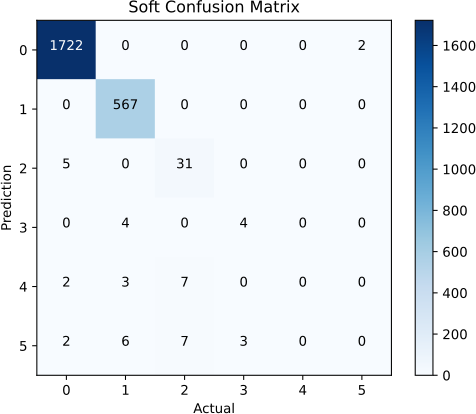
\includegraphics[width=\linewidth]{pics/soft_confusion_matrix.png}
        \caption{Die «weiche» Konfusionsmatrix mit absoluten werten (Anzahl Gelenke).}
    \end{subfigure}
    \hfill
    \begin{subfigure}{0.45\textwidth}
        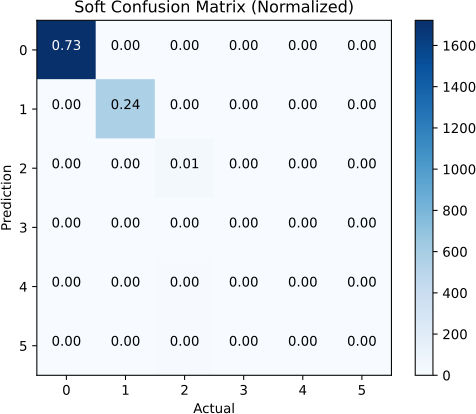
\includegraphics[width=\linewidth]{pics/soft_confusion_matrix_norm.png}
        \caption{Die «weiche» Konfusionsmatrix normalisiert.}
    \end{subfigure}
    \caption{Die verschiedenen Konfusionsmatrizen im Überblick.}
    \label{fig:konfusionsmatrizen}
\end{figure}

\subsubsection{Ergebnisse der Evaluation}

Die Evaluationsmetriken können mit einem Python-Skript berechnet und ausgegeben werden.\footnote{Siehe \texttt{deepxray/evaluation/evaluation/evaluation.py}. Die Ausgabe des Skripts ist in der Datei \texttt{evaluation/evaluation/evaluation.txt} zu finden.} Dabei werden folgende Ergebnisse ermittelt:

Die \textit{Global Accuracy} beträgt nach exaktem Vergleich $69.641\%$. Kommt Soft Matching zum Einsatz, beträgt sie $94.089\%$.

Die Ergebnisse der Metriken, die nach Klasse ermittelt werden, sind in \tblref{tbl:classaccuracies}; diejenigen, die auf \textit{Cohen's Kappa} basieren, in \tblref{tbl:cohenskappa} dargestellt.

\begin{table}[tbh]
    \center
    \begin{tabular}{l|l}
        Metrik & Ergebnis \\ \hline
        Class Accuracy (exakt) & $[0: 0.86, 1: 0.43, 2: 0.28, 3: 0.29, 4: 0.00, 5: 0.00]$ \\
        Class Accuracy (soft) & $[0: 0.99, 1: 0.98, 2: 0.69, 3: 0.57, 4: nan, 5: 0.00]$ \\
        Precision (exakt) & $[0: 0.86, 1: 0.43, 2: 0.28, 3: 0.29, 4: 0.00, 5: 0.00]$ \\
        Precision (soft) & $[0: 1.00, 1: 1.00, 2: 0.86, 3: 0.50, 4: 0.00, 5: 0.00]$ \\
        Recall (exakt) & $[0: 0.76, 1: 0.55, 2: 0.31, 3: 0.29, 4: nan, 5: 0.00]$ \\
        Recall (soft) & $[0: 0.99, 1: 0.98, 2: 0.69, 3: 0.57, 4: nan, 5: 0.00]$ \\
        F1-Score (exakt) & $[0: 0.80, 1: 0.48, 2: 0.29, 3: 0.29, 4: nan, 5: nan]$ \\
        F1-Score (soft) & $[0: 1.00, 1: 0.99, 2: 0.77, 3: 0.53, 4: nan, 5: nan]$ \\
    \end{tabular}
    \caption{Die Ergebnisse der klassenbasierten Evaluationsmetriken.}
    \label{tbl:classaccuracies}
\end{table}

\begin{table}[tbh]
    \center
    \begin{tabular}{l|r|r}
        Metrik & Ergebnis & Vertrauensintervall ($95\%$) \\ \hline
        Cohen's Kappa (exakt) & $0.324$ & $[0.283, 0.365]$ \\
        Cohen's Kappa (soft) & $0.957$ & $[0.945, 0.970]$ \\
        Cohen's Quadratic Kappa (exakt) & $0.449$ & $[0.443, 0.454]$ \\
        Cohen's Quadratic Kappa (soft) & $0.797$ & $[0.794, 0.801]$ \\
    \end{tabular}
    \caption{Die Ergebnisse der Evaluationsmetriken, die auf \textit{Cohen's Kappa} basieren.}
    \label{tbl:cohenskappa}
\end{table}

\subsubsection{Interpretation der Evaluationsergebnisse}

Bei den Konfusionsmatrizen (\imgref{fig:konfusionsmatrizen}) fällt auf, dass sich die Scores auf die beiden Klassen 0 (ca. $72\%$) und 1 (ca. $25\%$) konzentrieren. Vor diesem Hintergrund ist eine \textit{abschliessende} Interpration der Ergebnisse nicht angebracht. Für diese wären weitere Evaluationsdaten zu sammeln und zu verarbeiten. Dennoch können aus den verschiedenen Metriken einige Erkenntnisse gewonnen werden.

Die \textit{Global Accuracy} ist mit ca. $70\%$ (exakt) bzw. ca $94\%$ (soft) zwar hoch, aufgrund der unbalancierten Daten jedoch nicht aussagekräftig.\footnote{Hat die Mehrheit der Datenpunkte die Score 0, erreichte man mit einer statischen Prediction von 0 bereits eine Accuracy von über $50\%$.}

Bei den klassenbasierten Metriken fällt auf, dass für die Scores 4 und 5 keine Aussagen möglich sind. Tatsächlich lassen sich im Ergebnisdatensatz des Scorings nur zwei Gelenke mit der Score 5 und kein einziges der Score 4 finden.\footnote{Dies ist nicht \textit{nur} auf die \textit{false negatives} von \texttt{body\_part} zurückzuführen. So finden sich im ganzen Evaluationsdatensatz nur vier Gelenke der Score 4 und zwei der Score 5 (siehe Python-Skript \texttt{deepxray/test\_data/high\_scores.py}). Falsche Scores können auch auf eine fehlerhafte Gelenkextraktion hindeuten, zumal stark geschädigte Gelenke teilweise nicht mehr als solche zu erkennen sind.} Bei den Klassen von 0-3 fällt auf, dass die Übereinstimmungen bei den \textit{Soft Matches} durchgehend bedeutend höher ausfallen als diejenigen auf Basis exakter Vergleiche. Weiter gilt (mit wenigen geringfügigen Ausnahmen): Je höher die Score, desto unpräziser fallen die Predictions aus. Das könnte damit zu tun haben, dass die wenigen höheren Scores (Klassen 2 und 3) eher zufällig als systematisch übereinstimmen. Die \textit{Soft Matches} zeichnen hier ein etwas positiveres Bild, so beträgt die Übereinstimmung in den Klassen von 0 bis 3 zwischen $50\%$ und $100\%$ (gerundet).

Auch die Metriken \textit{Cohen's Kappa} und \textit{Cohen's Quadratic Kappa} hinterlassen einen gemischten Eindruck im Bezug auf die Performance. Diese fallen mit $0.324$ bzw. $0.449$ zu tief aus, dass der klinische Einsatz des Prototypen auch nur in Erwägung gezogen werden könnte.\footnote{\textit{«Any kappa below 0.60 indicates inadequate agreement among the ratorers and little confidence should be placed in the study results.»} \cite{interrater-reliability} Jedes Kappa unter 0.60 weist auf eine inadäquate Übereinstimmung unter den Bewertern hin, diesen Studienergebnissen sollte nur geringes Vertrauen entgegengebracht werden. (Übersetzung des Autors)}

Dass \textit{Cohen's Quadratic Kappa} grösser ausfällt als \textit{Cohen's Kappa} (jeweils in der exakten Variante), mag zunächst überraschen. Dies ist jedoch ein bekanntes statistisches Phänomen bei sogenannten \textit{tridiagonalen Tabellen}. Eine rechteckige Matrix (z.B. eine Konfusionsmatrix) ist tridiagonal, wenn nur in der Hauptdiagonalen (Übereinstimmungen) und in den beiden benachbarten Diagonalen (Sub- und Superdiagonalen) Werte auftauchen, die sich von null unterscheiden. Da es sich bei der Konfusionsmatrix in der vorliegenden Evaluation annähernd um eine tridiagonale Matrix handelt\footnote{Die Soft Matches, welche in den Haupt-, Sub- und Superdiagonalen zu liegen kommen, liegen ja weit über 90\%.}, ist der Unterschied zwischen den beiden Kappa-Metriken durchaus plausibel \cite{warrens-kappa}.

Auf Basis der \textit{Soft Matches} fallen die Kappas mit $0.957$ bzw. $0.797$ wesentlich höher aus. Dies könnte dahingehend interpretiert werden, dass der Prototyp zwar nicht sechs Klassen zuverlässig auseinanderhalten kann, jedoch in seinen Predictions nur geringfügige Abweichungen aufweist und immerhin für eine Unterscheidung zwischen tiefer, mittlerer und hoher Schädigung zuverlässig arbeitet. Aufgrund der Datenbasis mit sehr wenigen Daten in den höheren Klassen ist diese Interpretation jedoch voreilig.

\subsubsection{Anmerkung zu Soft Matches}
\label{sec:anmerkung-zu-soft-matches}

Die Soft Matches sind mit Vorsicht zu geniessen. Die menschlichen Scores liegen oft auf den Klassengrenzen der Predictions, z.B. liegt 20\% gerade auf der Grenze zwischen Klasse 1 ($]0\%..20\%]$) und 2 ($]20\%.. 40\%]$), gehört per Definition aber zur Klasse 1 \cite[S. 10]{rohrbach2017}. Somit sollte eine maschinelle Prediction legitimerweise den Scores 1 oder 2 zugeordnet werden ‒ zu 0 ($0\%$) und 3 ($]40\%..60\%]$) jedoch besser nicht. Die Soft-Match-Logik interpretiert jedoch nicht nur eine Score von 1 und 2, sondern auch von 0 als Übereinstimmung mit 20\%. Was bei einer menschlichen Score von 10\% durchaus sinnvoll wäre, schiesst bei Grenzfällen wie 20\% übers Ziel hinaus. Die Soft Matches arbeiten somit tendenziell zu grosszügig.

Um solche Grenzfälle in der Evaluation präziser behandeln zu können, müsste der Evaluationsworkflow Gebrauch der exakten menschlichen Scores machen. So könnte die \textit{Soft Confusion Matrix} beispielsweise für 10\% die Klassen 0, 1 und 2 als Treffer werten, für 20\% hingegen nur die Klassen 1 und 2. Dies dürfte zu präziseren ‒ und wohl etwas schlechter ausfallenden ‒ Soft-Metriken führen. Dieser erweiterte Evaluationsworkflow soll jedoch nicht im Rahmen der vorliegenden Arbeit umgesetzt werden.\footnote{Hierbei handelt es sich um einen klassischen Zielkonflikt: Der Data Miner möchte möglichst viele Daten zur Verfügung haben ‒ der Datenschützer möchte nur diejenigen zur Verfügung stellen, die für den jeweiligen Zweck unbedingt nötig sind. Der Projektmanager hingegen drängt auf den Abschluss der Evaluation, da noch eine Dokumentation zu schreiben ist.}

Die Toleranz der Abweichung könnte zudem empirisch bestimmt werden, indem die Abweichungen verschiedener menschlicher Scorer berücksichtigt werden. Hierfür stehen jedoch wissenschaftlich fundierte Metriken zur Verfügung (Stichwort \textit{Interclass Correlation}, ICC), sodass man vom Soft-Matching-Ansatz wegkommen könnte, stünden die Ergebnisse mehrerer menschlicher Scorer zur Verfügung.

\subsubsection{Fazit}

Der Evaluationsdatensatz ist unzureichend, um eine verbindliche Evaluation des Prototypen vornehmen zu können. Zwar weisen die Predictions für die tieferen Scores eine hohe Übereinstimmung auf, und die Abweichungen fallen betraglich eher gering aus. Für die höheren Klassen gibt es aber nur vereinzelte Datenpunkte, die keine signifikante Aussage zur Performance zulassen.

Wichtiger als ein solches Gesamturteil ist jedoch die Tatsache, dass ein weitgehend automatisierter Evaluationsworkflow mit verschiedenen Metriken umgesetzt worden ist, der in Zukunft mit weiteren Daten gefüttert und erneut ausgeführt werden kann. Schliesslich ist das Ziel der Evaluation nicht nur, eine einmalige Einschätzung des Systems vorzunehmen, sondern eine Möglichkeit zu haben, systematische Vergleiche zwischen verschiedenen Versionen des Systems anstellen zu können.

Für künftige Evaluationen ist zu beachten, dass neue und für Modellverbesserungen verwendete Trainingsdaten nicht mehr in der darauffolgenden Evaluation verwendet werden sollten.

\clearpage

\subsection{Evaluation der Zielerreichung}
\label{sec:evaluation-der-zielerreichung}

An dieser Stelle soll überprüft werden, ob und wie die Projektziele (siehe \secref{sec:erwartetes-resultat}) erreicht worden sind. Dies sind:

\begin{enumerate}
    \item \textit{Stand der Technik zur Industrialisierung (Evaluation, Testing) von ML-Modellen:} Dieses Thema wurde im Abschnitt \secref{sec:evaluation-von-modellen} auf Basis verschiedener Publikationen untersucht.
    \item \textit{Vorschlag für ein generisches Format von Modellen zum Exportieren aus ML-Frameworks und zum Importieren zur Ausführung:} Diese Problematik wurde in Abschnitt \secref{sec:modellformate} behandelt. Mittelfristig dürfte das SavedModel-Format von TensorFlow besser geeignet sein als das Format der ONNX-Initiative.
    \item \textit{Vorschlag für geeignete Metriken zum Vergleich von Modellen:} Hierzu wurden allgemeine Metriken (Accuracy, Precision, Recall, F1-Score) als auch domänenspezifische (Cohen's Kappa) gefunden (siehe \secref{sec:evaluationsmetriken}).
    \item \textit{Aufzeigen, was für eine Verheinheitlichung der Codebasis gemacht werden muss}: Diese Fragestellung wird im Ausblick behandelt (siehe \secref{sec:aktualisierung-auf-aktuelle-versionen}).
    \item \textit{Lauffähiger Prototyp}: Der Prototyp funktioniert und ist im Kapitel \secref{sec:realisierung} ausführlich dokumentiert.
    \begin{enumerate}
        \item \textit{Automatisierte Evaluation und Testing von neuen Modellen mit Vergleich zu alten Modellen und Minimum-Standards}: Der Evaluationsworkflow wurde umgesetzt, mit einem Evaluationsdatenset durchgeführt und ist in Abschnitt \secref{sec:technische-evaluation} dokumentiert.
        \item \textit{Visualisierung und Reporting der Performanz neuer Modelle}: Die Performanz kann über den Evaluationsworkflow (siehe wiederum \secref{sec:technische-evaluation}) ausgewertet werden. Als Visualisierung dienen verschiedene Konfusionsmatrizen (siehe \imgref{fig:konfusionsmatrizen}). Ein zusätzlich erstelltes Histogramm ist leider nur wenig aussagekräftig.
        \item \textit{API zum Ausführen des Modelles (Verteilen über mehrere GPUs)}: Die verschiedenen Modellkomponenten interagieren über eine Schnittstelle, die in Kapitel \secref{sec:realisierung} dokumentiert und auf \tblref{tbl:schnittstellen} übersichtlich zusammengefasst ist. Die Verteilung auf mehrere GPUs wurde nicht unternommen, da bereits mit CPUs eine akzeptable Performance erreicht werden konnte.
        \item \textit{Load Balancing, Messaging Systems}: Diese Thematik wurde in der Architekturdiskussion (\secref{sec:architekturvarianten}) ausführlich behandelt. Die verschiedenen Varianten für Messaging-Systeme werden kurz im Anhang evaluiert (siehe \secref{sec:wahl-der-message-queue}).
        \item \textit{Nahtloses Austauschen von alten Modellen mit neuen Versionen}: Die Austauschbarkeit kann nicht auf Modellebene, jedoch auf der Ebene der Modell\textit{komponenten} gewährleistet werden. Die Schnittstellen sind in \tblref{tbl:schnittstellen} zu finden.
    \end{enumerate}
\end{enumerate}

Fazit: Die wichtigsten Projektziele konnten erreicht werden. Dass die Austauschbarkeit der Machine-Learning-Modelle nicht auf Modellebene stattfinden konnte, zeichnete sich schon früh im Projektverlauf ab. Entsprechend wurde der Fokus früh auf die Austauschbarkeit von Modellkomponenten über definierte Schnittstellen gelegt. Im Bereich Visualisierung/Reporting wurde vergleichsweise wenig Aufwand investiert. Dafür musste zusätzliche Zeit investiert werden, um ein Modell neu zu trainieren, wofür die Modelldaten nicht mehr aufzufinden waren. Auch das Selektieren und Aufbereiten der Evaluationsdaten verursachte zusätzlichen Aufwand.

\subsubsection{Rückblick auf Projektrisiken}

Die zu Beginn des Projekts aufgestellten Projektrisiken (siehe \secref{sec:projektrisiken}) sollen an dieser Stelle wieder aufgegriffen werden. Sind Risiken eingetreten, und wenn ja, welchen Einfluss hatte dies auf den Projektverlauf? Haben sich die vorgeschlagenen Mitigationsmassnahmen als sinnvoll erwiesen?

\begin{description}
    \item[Keine lauffähigen Modelle] Dieses Risiko ist teilweise eingetreten, denn die Modelldaten zum \texttt{ratingen\_score}-Modell waren nicht mehr auffindbar. Die Mitigationsmassnahme, das Modell neu zu trainieren, konnte den Schaden eingrenzen. Dabei ist zwar Mehraufwand entstanden, das Projekt wurde dadurch aber nur unwesentlich verzögert.
    \item[Aktualisierung der Modelle] Dieses Risiko ist eingetreten, sodass die Aktualisierung der Modelle schon früh im Projektverlauf aufgegeben worden ist. Die Mitigationsmassnahmen (Isolation der bestehenden Modelle) haben sich als zielführend erwiesen. Der Prototyp konnte auf Basis der bestehenden Modelle umgesetzt werden.
    \item[Schlechte Performance (Prediction)] Die technische Evaluation lässt hier (noch) kein eindeutiges Urteil zu. Die Predictions bewegen sich ganz klar nicht im reinen Zufallsbereich, dürften aber für einen Produktiveinsatz noch zu wenig präzise sein. Dieses Risiko wird vom Auftraggeber getragen.
    \item[Schlechte Performance (Laufzeit)] Die Verarbeitungsgeschwindigkeit des Prototypen ist akzeptabel, wenn auch nicht berauschend. Die Anwendung ist skalierbar, sodass sich Hardwareerweiterungen (zusätzliche CPUs) und -verbesserungen (schnellere CPUs) positiv auf die Performance auswirken dürften.
    \item[Hoher Arbeitsspeicherverbrauch] Das Gesamtsystem benötigt mindestens 2 GB Arbeitsspeicher (eine Instanz pro Modellkomponente). Empfohlen sind 6 GB oder besser 11 GB (für fünf bzw. zehn laufende Instanzen der Gelenkextraktion). Diese Anforderungen stellen angesichts gegenwärtiger Speicherpreise kein Problem dar. Der Speicherbedarf ist jedoch kritisch, wenn die Modelle auf einer oder mehreren GPUs ausgeführt werden sollen.
\end{description}

Auf die Risiken, die für die einzelnen Projektphasen ermittelt worden sind (siehe \secref{sec:projektphasen}), soll an dieser Stelle nicht weiter eingegangen werden. Diese wurden jeweils ‒ falls nötig ‒ in der Reflexion der einzelnen Projektphasen kurz behandelt.

Obwohl einige der ermittelten Projektrisiken eingetreten sind, wurde der Erfolg des Projekts dadurch nicht beeinträchtigt. Die Mitigationsmassnahmen haben sich als sinnvoll und ausreichend erwiesen.

\newpage

\section{Ausblick}

Nach einem Semester der Recherche, Konzeption, Umsetzung und Dokumentation liegt als Projektergebnis ein lauffähiger, gut dokumentierter und skalierbarer Prototyp vor, der bei weitem noch nicht den Anforderungen für einen Produktiveinsatz genügt. Hierzu wäre noch einiges an Arbeit zu leisten, worauf im Abschnitt \secref{sec:ungeloeste-probleme} näher eingegangen wird. Im Abschnitt \secref{sec:weitere-ideen} sollen weitere Möglichkeiten besprochen werden, wie der entwickelte Prototyp in Zukunft erweitert und verbessert werden könnte.

Zunächst soll aber das im Rahmen der Bachelorarbeit Geleistete reflektiert werden.

\subsection{Reflexion der Arbeit}

Zu Beginn der Arbeit traten einige Schwierigkeiten im Zusammenhang mit den gegebenen Modellen auf. Diese mussten zunächst wieder zum Laufen gebracht und teilweise sogar neu trainiert werden. Der Projekterfolg stand zu diesem Zeitpunkt in Frage. Der definitive Projektauftrag konnte erst zum spätmöglichsten Zeitpunkt erteilt werden.

Die Modelle konnten zudem nicht einfach für eine aktuelle Laufzeitumgebung konvertiert werden. Dies wäre sehr aufwändig gewesen und hätte den zeitlichen Rahmen des Projekts gesprengt. Stattdessen wurde die Entscheidung gefällt, die bestehenden Modelle in einer isolierten Laufzeitumgebung anzubieten. Die verschiedenen Modelle konnten so in der ersten Projektphase doch noch zum Laufen gebracht werden.

In der zweiten Projektphase wurde viel recherchiert und konzipiert. Der Projektfortschritt war in dieser Phase nicht offensichtlich, da die verschiedenen Architekturvarianten v.a. im Kopf des Autors und auf Notizpapier ausgearbeitet worden sind. Um bei der Zwischenpräsentation nicht nur ein reines Theoriekonstrukt demonstrieren zu müssen, wurde ein Prototyp mit simulierten Modellkomponenten entwickelt.\footnote{siehe \url{https://github.com/patrickbucher/fake-x-ray} (abgerufen am 26.05.2020)}

Dieser «Fake-Prototyp» erwies sich als Glücksfall, zumal dessen Architektur grösstenteils für die Entwicklung des \textit{eigentlichen} Prototypen übernommen werden konnte. Die Entwicklung desselben ging dann v.a. während zweier Wochenenden vonstatten, wonach nur noch geringfügige Verbesserungen vorgenommen worden sind.

Die Recherche, Wahl und Umsetzung der Evaluationsmetriken nahm mehr Zeit in Anspruch als erwartet. Auch mussten die Evaluationsdaten in verschiedenen Schritten aufbereitet und selektiert werden. Dank der schnellen Fortschritte beim Prototyp führten diese Aufwände jedoch zu keiner Verzögerung im Projekt.

Auf Basis einer pragmatischen und differenzierten Teststrategie wurden zwar eher wenige und kleine, dafür aber aussagekräftige automatisierte Tests umgesetzt. So kommen bei der Evaluation Unittests (mit hoher Codeabdeckung), bei den Modellkomponenten Integrationstests und für den \texttt{orchestrator} (bzw. für das Gesamtsystem) Systemtests (End-to-End) zum Einsatz.

Die Dokumentation hinkte dem Projektfortschritt über die meiste Zeit etwas hinterher, war aber zum Schluss des Projekts doch recht schnell geschrieben. Hier erwiesen sich die Erfahrungen des Wirtschaftsprojekt (sowie das damals erstellte \LaTeX{}-Template) als sehr nützlich.

Das Projektergebnis ist für den Autor sehr zufriedenstellend ausgefallen und schafft für den Auftraggeber eine solide Basis für die künftige Weiterentwicklung.

\subsubsection{Lessons Learned}

\begin{enumerate}
    \item Das systematische Nachdenken über Architekturentscheidungen mit verschiedenen Varianten mag in einer Zeit, die «Agilität» als höchstes Ideal preist, als überholt erscheinen und etwas nach V-Modell anmuten. Es kann jedoch wesentlich effektiver und effizienter sein, möglichen Problemen durch ungestörtes Nachdenken auf die Spur zu kommen, als diese erst nach dem Ende mehrerer Sprints (in die falsche Richtung) erkennen zu müssen.
    \item Eine Software muss zwecks Qualitätsicherung systematisch getestet werden. Systematisch heisst jedoch nicht, dass jeder Aspekt der Software mit dem gleichen (Unittests), sondern mit einem auf das jeweilige Problem passenden Werkzeug (Unittests, Integrationstests, Systemtests, manuelle Tests usw.) Werkzeug getestet werden soll. Ein schlanker End-to-End-Test ist oft aussagekräftiger, stabiler und besser wartbar als eine Ansammlung von Unittests mit Mocks und Test-Doubles.
    \item Obwohl es sich bei der vorliegenden Arbeit eher um ein Softwareentwicklungs- als um ein Machine-Learning-Projekt  handelt, war ein grundlegendes Verständnis von Machine-Learning-Konzepten nötig, v.a. bei der Evaluation. Auch grundlegende Kenntnisse der Domäne (Scoring von Röntgenbildern, rheumatoide Arthritis) haben sich als extrem wichtig erwiesen, so konnte etwa eine Unstimmigkeit in der Struktur der Evaluationsdaten über die Sichtung einiger Röntgenbilder erkannt und behoben werden.
\end{enumerate}

\subsubsection{Verwendete Werkzeuge}

Zur Entwicklung des Prototyps wurden die Programmiersprachen Go und Python verwendet. Als wichtige Libraries (die gegebenen Machine-Learning-Frameworks ausgenommen) kamen u.a. AMQP, UUID (Go) sowie NumPy, Pandas, SciPy Stats, Requests, PyTest und Pika (Python) zum Einsatz. Die Werkzeuge \texttt{make}, \texttt{bash} und \texttt{jq} erwiesen sich an verschiedenen Stellen als sehr hilfreich. 

Der Prototyp macht regen Gebrauch von Docker und kann am einfachsten mit Docker Compose ausgeführt werden. RabbitMQ hat sich als sehr robuste und einfach zu handhabende Messaging-Lösung erwiesen.

Der Bericht und das Web-Abstract wurden mit \LaTeX{} bzw. \XeLaTeX{} gesetzt. Für das Arbeitsjournal kamen Markdown und Pandoc zum Einsatz. Die PDF/A-Konformität der Dokumente wurde mit Ghostscript sichergestellt. Die UML-Diagramme wurden mit PlantUML erstellt. Für weitere Grafiken kam Graphviz zum Einsatz.

Das Video wurde mit \texttt{ffmpeg} aufgenommen. Die Tonspur wurde mit Audacity aufgenommen, abgemischt und wiederum mit \texttt{ffmpeg} mit dem Video kombiniert.

Quellcode und Dokumentation wurden ausschliesslich in \texttt{vim} geschrieben. Plugins wie \texttt{vim-go} und \texttt{python-mode} machen diesen flexiblen Texteditor zu einer komfortablen Entwicklungsumgebung.

Sämtliche Quellcode- und Textartefakte wurden mit Git verwaltet und regelmässig zusammen mit Modell- und Testdaten mithilfe von \texttt{restic} auf einen externen Datenträger gesichert.

\subsection{Ungelöste Probleme}
\label{sec:ungeloeste-probleme}

Obwohl die Projektziele erreicht worden sind (siehe \secref{sec:evaluation-der-zielerreichung}), bleibt noch einiges zu tun, damit der Prototyp dereinst produktiv eingesetzt werden kann. Im Verlauf der Arbeit wurden folgende ungelöste Probleme gesammelt und vom Rahmen der Bachelorarbeit abgegrenzt:

\begin{description}
    \item[Modelle aktualisieren] Die bestehenden Machine-Learning-Modelle sollen auf eine aktuelle Version von TensorFlow aktualisiert werden. Diese Problematik wird ausführlicher im Abschnitt \secref{sec:aktualisierung-auf-aktuelle-versionen} behandelt.
    \item [Deployment der Container] Beim Auftraggeber (Seantis GmbH) kommen zwar Container zum Einsatz, die auf Docker-Images basieren. Diese werden jedoch nicht mit der Docker-Runtime, sondern mit \texttt{systemd-nspawn} ausgeführt.\footnote{Die Gründe für und Vorteile dieses Ansatzes sind vielfältig \cite{docker-vs-systemd}.} Auch verfügt der Auftraggeber über ein eigenes Container-Buildsystem, in welches die erstellten Container integriert werden müssten. Der bisherige Ansatz mit Docker Compose ist nur für Test- und Demozwecke geeignet.
    \item [Continuous Integration] Die verschiedenen Unit-, Integrations- und Systemtests wurden während der Entwicklung des Prototyps jeweils manuell ausgeführt. Für eine produktive Weiterentwicklung der Software wäre die Integration der Test-Pipeline in das CI-System des Auftraggebers angebracht. Dieses basiert auf Buildkite.\footnote{siehe \url{https://buildkite.com/} (abgerufen am 26.05.2020)} Um dieses System effektiv nutzen zu können, wäre wohl auch die Aufteilung des bisherigen Git-Repositories in mehrere Repositories (eines pro Komponente) sinnvoll.
    \item [Security] Für eine produktive Anwendung, die mit schützenswerten Daten wie Röntgenbildern umgeht, gelten andere Sicherheitsanforderungen als für einen Prototyp. Für die Kommunikation zwischen dem Client und dem \texttt{orchestrator} dürfen keine selbst signierten, sondern nur von einer Zertifizierungsstelle ausgestellten TLS-Zertifikate verwendet werden. Die Message-Queues sind über geeignete Massnahmen zu schützen, indem diese nur intern zugänglich gemacht oder durch zureichende Authentifizierungs- und Autorisierungsmechanismen geschützt werden.
    \item [i.i.d.-Hypothese] Die Trainings- und Evaluationsdaten müssen der i.i.d.-Hypothese (independent, identically distributed) genügen, das heisst unabhängig voneinander sein und der gleichen Verteilung folgen. Diese Hypothese konnte im Rahmen der Bachelorarbeit nicht geprüft werden. Es gibt mögliche Hinweise darauf, dass diese Hypothese für die verwendeten Röntgenbilder nicht zutreffen könnte. Zum einen sind schwere Krankheitsverläufe der rheumatoiden Arthritis aufgrund verbesserter Früherkennung und Therapiemassnahmen immer seltener. Die betroffenen Patienten sterben zusehends weg, was zu einer laufenden Verschiebung der Ratingen-Scores nach unten führen wird. Andererseits werden in der SCQM-Datenbank auch die Krankheitsverläufe der gleichen Patienten verfolgt, d.h. die stetig fortschreitenden (da irreversiblen) Schädigungen an Gelenken führen im Verlauf der Langzeitstudien zu Ratingen-Scores, die ansteigen oder bestenfalls stagnieren. Ob und inwiefern sich diese Verschiebungen mit der laufenden Aufname von Daten neuer Patienten in die SCQM-Datenbank ausgleicht, kann nur mit einer systematischen statistischen Untersuchung ermittelt werden.
    \item [Gleichbleibende Predictions] Ein oft genannter Vorteil des automatischen Scorings von Röntgenbildern gegenüber menschlichen Scorern ist, dass der erste Ansatz eine konstante Qualität der Predictions gewährleistet. Dies gilt jedoch nur, solange die Modelle unverändert zum Einsatz kommen. Werden diese durch neuere, verbesserte Versionen ersetzt, würden für bestehende Daten wohl andere Scores resultieren. Bei diesem Zielkonflikt ‒ konstante oder möglichst genaue Scores ‒ gilt es aufseiten des Auftraggebers die Prioritäten festzulegen.
    \item [Evaluation] In \secref{sec:verschiedene-datentypen} wurde für das Modell \texttt{ratingen\_score} erwähnt, dass die Evaluation nicht nur auf Basis einzelner Gelenke stattfinden soll, sondern dass auch die Anzahl erkannter Gelenke pro Röntgenbild ein mögliches Qualitätskriterium sei. Diese Evaluationsmetrik wurde nicht umgesetzt. Diese Metrik würde Rückschlüsse auf die Qualität des Modells \texttt{joint\_detection} erlauben.
\end{description}

\subsubsection{Aktualisierung der Modelle}
\label{sec:aktualisierung-auf-aktuelle-versionen}

Die verschiedenen Machine-Learning-Modelle basieren auf älteren Versionen von TensorFlow und anderen Libraries/Frameworks (hier als \textit{Packages} zusammengefasst). \tblref{tbl:versionen} bietet einen Überblick über die verwendeten und derzeit aktuellen Versionen.

\begin{table}[H]
    \center
    \begin{tabular}{l|l|l|l}
        Modell & Package & eingesetzt & aktuell \\ \hline
        \texttt{body\_part} & \texttt{tflearn} & \texttt{0.2.1} & \texttt{0.3.2} \\
        \texttt{joint\_detection} & \texttt{tensorflow} & \texttt{0.12.1} & \texttt{2.2.0} \\
        \texttt{joint\_detection} & \texttt{scipy} & \texttt{0.18.1} & \texttt{1.4.1} \\
        \texttt{joint\_detection} & \texttt{Pillow} & \texttt{3.4.2} & \texttt{7.1.2} \\
        \texttt{ratingen\_score} & \texttt{tensorflow} & \texttt{1.4.0} & \texttt{2.2.0} \\
        \texttt{ratingen\_score} & \texttt{scikit-learn} & \texttt{0.22.2.post1} & \texttt{0.23.1} \\
    \end{tabular}
    \caption{Die verwendeten Versionen verschiedener Machine-Learning-Packages sind grösstenteils veraltet.}
    \label{tbl:versionen}
\end{table}

Um das Ausmass der nötigen Änderungen für eine Aktualisierung auf neuere Packages besser abschätzen zu können wurde folgendermassen verfahren:

\begin{enumerate}
    \item Die Modellkomponenten wurden in ein eigenes Arbeitsverzeichnis kopiert.
    \item Die \texttt{Dockerfile}s, die auf älteren Versionen von Python basieren, wurden gelöscht. Schliesslich sollen die Modellkomponenten mit einer aktuellen Version von Python, d.h. auch ausserhalb eines Containers, betrieben werden können.
    \item Stattdessen wurde pro Modellkomponente eine neue virtuelle Python-Umgebung basierend auf Python 3.8.3 erstellt.
    \item In den \texttt{requirements.txt}-Dateien wurden sämtliche Versionsangaben entfernt, sodass die jeweils neueste Version der Packages installiert wird.
    \item Damit die Modellkomponenten überhaupt aufgestartet werden können, wurde eine Instanz von RabbitMQ im Hintergrund gestartet.
    \item Es wurde versucht, die einzelnen Einstiegspunkte der Modellkomponenten (Hauptklasse) aufzustarten. Dabei aufgetretene Fehlermeldungen wurden nachgeschlagen.
    \item Der Integrationstest im \texttt{tests/}-Unterverzeichnis wurde via \texttt{pytest} (nicht via Docker!) aufgestartet; Fehlermeldungen wiederum nachgeschlagen.
\end{enumerate}

Für die aufgetretenen Fehlermeldungen werden möglichen Lösungsansätze skizziert. Hierzu sollen pro Modellkomponente höchstens eine Stunde aufgewendet werden. Dieser Ausblick kann nur eine Idee über das Ausmass der anstehenden Arbeiten, jedoch keine ausführlichen Arbeitsanleitungen liefern. Demnach gibt es für die Aktualisierung der Modelle folgendes zu tun:

\begin{description}
    \item [\texttt{body\_part}] Das Unterpackage \texttt{contrib} wurde für TensorFlow Version 2 entfernt. Dieses kann nur zusammen mit TensorFlow 1 verwendet werden, was nicht im Sinne einer Aktualisierung ist. \texttt{tflearn} bietet derzeit keine Unterstützung für TensorFlow 2.0.\footnote{\url{https://github.com/tflearn/tflearn/issues/1121} (abgerufen am 26.05.2020)} Da diese Situation nun schon seit über einem Jahr besteht, wäre die Umstellung von \texttt{tflearn} auf Keras wohl die bessere Variante als das Warten auf eine neue \texttt{tflearn}-Version mit Unterstützung für TensorFlow 2. Hierfür müsste der Code grösstenteils neu geschrieben und das Modell neu trainiert werden, was auch mit dem bekannten Problem der Modellformate (siehe \secref{sec:modellformate}) zu tun hat. Das zugrundeliegende Modell \textit{Inception V3} kann auch für Keras verwendet werden.\footnote{\url{https://keras.io/api/applications/inceptionv3/} (abgerufen am 26.05.2020)} Die Änderungen beschränken somit auf das Ansprechen der High-Level-API, da das Modell konzeptionell (Definition der Layer) übernommen werden kann.
    \item [\texttt{joint\_detection}] Hier kommt nicht \texttt{tflearn}, sondern die «rohe» API von TensorFlow zum Einsatz. Es muss somit nicht auf eine komplett andere, sondern bloss auf eine neuere API migriert werden. Rein technisch kommt Version 0.12.1 zum Einsatz. Dies war die letzte Minor-Version vor dem 1.0-Release. Zur Migration von TensorFlow 1 auf 2 gibt es einen offiziellen und umfassenden Guide.\footnote{\url{https://www.tensorflow.org/guide/migrate} (abgerufen am 26.05.2020)}. Ob dieser auch für eine Migration von der Version 0.12.1 auf die aktuelle Version 2.2.0 funktioniert, müsste ausprobiert werden. Hier wäre ein Ausweichen auf die Keras-API wohl einfacher. Die \texttt{joint\_detection}-Modelle basieren auf dem Modell \textit{Inception V1}. Dieses arbeitet weniger genau und langsamer als die aktuelleren Varianten V2 und V3.\footnote{\url{https://towardsdatascience.com/a-simple-guide-to-the-versions-of-the-inception-network-7fc52b863202} (abgerufen am 26.05.2020) bietet einen Vergleich der verschiedenen Versionen.} Dieses Basismodell wird nicht über ein Package, sondern direkt als Code (\texttt{joint\_detection/legacy/utils}) zur Verfügung gestellt. Eine Umstellung auf Inception V3 würde diesen und weiteren Code im \texttt{utils/}-Unterverzeichnis (inklusive einigen C++-Code und die Library \texttt{stitch\_wrapper.so}) obsolet machen. Das Umschreiben des TensorFlow-Codes würde sich so auf die Klasse \texttt{JointDetectionModel} und auf den Trainingscode beschränken. Alternativ kann Inception V3 auch über die Keras-API verwendet werden, was ganz im Sinne der Vereinheitlichung des Modell-Codes wäre.
    \item [\texttt{ratingen\_score}] Hierbei handelt es sich um das neueste Modell, das dementsprechend auch auf einer aktuelleren API von TensorFlow (Version 1.4.0) basiert. Hier wird TensorFlow über die Keras-API angesprochen, wodurch die Aktualisierung auf TensorFlow 2.2.0 keine grösseren Probleme verursachen sollte. Auch das Inception-Basismodell wird in der aktuellen Version 3 verwendet. Zudem ist diese Modellkomponente die einzige ohne Legacy-Code, wodurch keine zusätzliche Arbeit zum Portieren von Code anfällt. Ein erster Versuch der Aktualisierung auf TensorFlow 2.2.0 verlief vielversprechend. Die Laufzeitumgebung beschwerte sich einzig über den eingesetzten Adam-Optimizer. Die Modellkomponente konnte jedoch ohne diesen zum Laufen gebracht werden. Detaillierte Tests im Bezug auf die Qualität der Predictions und auf die Laufzeitperformance wurden jedoch keine unternommen. Solche könnten jedoch mit den Code-Artefakten aus dem GitHub-Repository\footnote{\url{https://github.com/janickrohrbach/arthritis-net} (abgerufen am 26.05.2020)} ohne grossen Aufwand unternommen werden.
\end{description}

Fazit: Die beiden Modellkomponenten \texttt{body\_part} und \texttt{joint\_detection} sollten über die Keras-API auf TensorFlow 2 aktualisiert werden. Bei letzterem sollte zusätzlich vom Basismodell Inception V1 auf Inception V3 umgestellt werden. Das Modell \texttt{ratingen\_score} sollte sich problemlos auf TensorFlow 2 aktualisieren lassen, zumal es schon die Keras-API verwendet. (Dieses Modell war schliesslich nicht der Grund dafür, dass die Aktualisierung der Modelle nicht in den Umfang der Bachelorarbeit aufgenommen worden ist.)

\subsection{Weitere Ideen}
\label{sec:weitere-ideen}

An dieser Stelle sollen noch einige Ideen skizziert werden, die im Verlauf der Arbeit aufgekommen sind, jedoch klar ausserhalb des Projektscopes liegen und für diesen nie in Betracht gezogen worden sind.

\begin{description}
    \item [Rau-Score] Die Ratingen-Score bezieht sich auf die Schädigung eines einzelnen Gelenks. Mit der Rau-Score werden die Schädigungen verschiedener Gelenke (je elf an den beiden Händen, d.h. MCP 1-5, PIP 1-5 und das Handgelenk; sowie fünf Gelenke pro Fuss) zu einer einzigen Score zusammengefasst, die den Fortschritt der Erkrankung bei einem Patienten in einer einzigen Zahl zusammenfasst. Um diese Rau-Score berechnen zu können, müssten zusätzlich das Handgelenk sowie die Gelenke an den Füssen verarbeitet werden können. Die Berechnung der Rau-Score wäre dann trivial.
    \item [Optische Aufbereitung] Bei der Web-Oberfläche wäre es sehr hilfreich, wenn die detektierten und gescorten Gelenke direkt mit einem farbigen Rahmen ‒ von grün, keine Schädigung, bis rot, starke Schädigung ‒ hervorgehoben werden könnten. Das Nachschauen an drei Orten ‒ Röntgenbild, Liste der Scores und Legende ‒ könnte so entfallen. Um dies umsetzen zu können, müsste die Modellkomponente \texttt{joint\_detection} zusätzlich die ermittelten Bildkoordinaten der detektierten Gelenk zurückliefern, sodass diese anschliessend umrahmt werden könnten. Hierzu müsste die API erweitert werden. Dies könnte einerseits über einen weiteren Endpoint geschehen, oder mithilfe eines \texttt{Accept}-Headers, womit zwischen \texttt{image/jpeg} (für eine annotierte Grafik) und \texttt{ap\-pli\-ca\-tion/json} (für den bestehenden JSON-Payload) unterschieden würde.
    \item [Implementierung in Erlang] Recherchen zum Message-Broker RabbitMQ haben den Autor auf dessen zugrundeliegende Programmiersprache \textit{Erlang} aufmerksam gemacht. Zwar konnte der \texttt{orchestrator} dank der hervorragenden Concurrency-Me\-cha\-nis\-men von Go problemlos umgesetzt werden. Mit Erlang, das auf dem \textit{Actor}-Modell basiert, würden sich derlei Orchestrierungsprobleme wohl noch eleganter lösen lassen. So könnten die verschiedenen Modellkomponenten mit ihrer Anbindung an RabbitMQ als Actors abstrahiert werden. Der Nachrichtenfluss könnte dann mit einer deklarativen, auf Prolog basierenden Syntax einfach und übersichtlich zwischen diesen Actors definiert werden. Die Unterstützung dafür benötigter Technologien wie HTTP, JSON usw. wäre über die OTP gewährleistet.\footnote{Weitere Informationen zu Erlang finden sich auf der offiziellen Webseite (\url{https://erlang.org/doc/}, abgerufen am 26.05.2020), sowie in Joe Armstrongs Einführungsbuch \cite{programming-erlang} und Doktorarbeit \cite{armstrong2003}.} Die Reimplementierung der \texttt{orchestrator}-Komponente böte eine schöne Fallstudie zum Vergleich der Concurrency-Modelle von Go (CSP) und Erlang (Actor-Modell) ‒ und ein praxisnahes Erlang-Lernprojekt.
\end{description}


\newpage

\section{Anhang}

Im Anhang werden folgende Inhalte gesammelt:

\begin{description}
    \item[Technologieevaluation] Die Wahl der Programmiersprache ‒ bzw. der Programmier\textit{spra\-chen}, da verschiedene zum Einsatz kommen ‒ wird anhand definierter Kriterien für die verschiedenen Einsatzbereiche (Komponenten) begründet. Auch die Wahl des Messaging-Protokolls und des Message-Brokers wird kurz begründet.
    \item[Schnittstellen] Die Schnittstellen zwischen den verschiedenen Komponenten werden in einem kurzen, tabellarischen Überblick zusammengefasst.
    \item[Abgabe] Abgegebene Artefakte wie Quellcode und Modelldaten, und weitere Inhalte, die nicht in den Bericht (dieses Dokument) eingefügt worden sind, werden hier aufgeführt.
\end{description}

\subsection{Wahl der Programmiersprache(n)}
\label{sec:wahl-der-programmiersprache}

Die Wahl der Programmiersprache ist in der vorliegenden Arbeit durch die vorgegebenen Modelle teilweise eingeschränkt. Bei anderen Komponenten, d.h. beim \texttt{orchestrator} und bei der Evaluation, bestehen grundsätzlich keine solchen Einschränkungen.

Wo eine Programmiersprache gewählt werden kann, soll dies nach den folgenden Kriterien geschehen:

\begin{description}
    \item[Domäne] Die Programmiersprache muss zum jeweiligen Einsatzbereich passen. \footnote{Bei Projekten mit einem Hintergrund in der Data Science und im Machine Learning wären etwa Python und R sinnvolle Varianten. Bei der Entwicklung hochperformanter Serversysteme kommen eher C, C++, Rust und Go zum Einsatz.}
    \item[Erfahrung] Der Autor der vorliegenden Arbeit soll bereits Erfahrung mit der jeweiligen Programmiersprache haben, d.h. bereits nicht-triviale Software damit entwickelt haben. Diese Erfahrung sollte nicht zu weit zurückliegen.\footnote{Kandidaten hierfür wären Java, Python, JavaScript, Go und R.}
    \item[Kompatibilität] Die Programmiersprache muss zu den bereits gesetzten und ausgewählten Technologien kompatibel sein.\footnote{Dies sind je nach Komponente u.a. TensorFlow, HTTP, JSON, Messaging.}
    \item[Perspektive] Es soll eine Programmiersprache gewählt werden, deren Alter und Popularität darauf hindeuten, dass sie in den nächsten fünf bis zehn Jahren noch gebräuchlich sein wird.\footnote{Der \textit{Lindy Effect} \cite{goldman1964} besagt, dass sich die Lebenserwartung nicht-verderblicher Sachen wie z.B. Technologien proportional zu deren Alter verhält. Rust, das am 15. Mai 2015 in Version 1.0 erschienen ist, und seither an Popularität gewinnt, hätte demnach noch eine Mindestlebenserwartung von fünf Jahren. Bei Go, das am 28. März 2012 in Version 1.0 herausgegeben worden ist, dürften es somit noch mindestens acht Jahre sein. Bei Nim, das am 23. September 2019 in Version 1.0 erschienen ist, darf man hingegen nur mit einer Mindestlebenserwartung von neun Monaten rechnen.} Dadurch kann die Anwendung über längere Zeit gewartet und muss nicht schon bald in grossen Teilen in einer anderen Programmiersprache neu entwickelt werden.
\end{description}

\subsubsection{Modellkomponenten \texttt{body\_part}, \texttt{joint\_detection}, \texttt{ratingen\_score}}
\label{sec:wahl-der-programmiersprache-modellkomponenten}

Da die Modelle in älteren Versionen von TensorFlow implementiert worden sind, lassen sich die Modelldaten nicht einfach für die Ausführung in einer anderen Laufzeitumgebung exportierten. Darum sollen sie in einem Container ausgeführt werden, der ihre ursprüngliche Laufzeitumgebung abbildet (siehe \secref{sec:bestehende-modelle} und \secref{sec:austauschbarkeit-von-modellen}).

Der Code zur Beschreibung der Modelle soll darum ebenfalls beibehalten werden. Somit kommt für die Komponenten, welche die Machine-Learning-Modelle anbieten, Python zum Einsatz.\footnote{Die Modelle \texttt{body\_part} und \texttt{joint\_detection} sind in einer Umgebung mit Python 3.6 entwickelt worden. Das neuere Modell \texttt{ratingen\_score} wurde auf einer Umgebung trainiert, welche die etwas ältere Version Python 3.5 erforderte. Python 3.6 unterscheidet sich v.a. durch neue Features von Python 3.5, wovon \textit{PEP 498: formatted string literals} das einzige Feature ist, das der Autor dieser Zeilen regelmässig verwendet (siehe \url{https://docs.python.org/3/whatsnew/3.6.html} für detaillierte Release-Informationen).} Somit ist Python 3.6 für die Komponenten \texttt{body\_part} und \texttt{joint\_detection}; und Python 3.5 für die Komponente \texttt{ratingen\_score} gesetzt.

\subsubsection{Neue Komponente \texttt{orchestrator}}
\label{sec:wahl-der-programmiersprache-orchestrator}

Für den \texttt{orchestrator} gelten andere Anforderungen als für die Modellkomponenten. Da für diese Komopnente noch kein Code existiert, kann diese komplett von Grund auf und ohne Technologieeinschränkungen aufgrund geleisteter Vorarbeiten entwickelt werden. Als Schnittstelle muss nicht nur eine Message-Queue unterstützt, sondern auch HTTP angeboten werden. Die grösste Schwierigkeit beim \texttt{orchestrator} besteht darin, dass dieser mit mehreren Anfragen gleichzeitig umgehen können muss, ohne dass die nebenläufigen Vorgänge (Gelenkextraktion und -scoring) dabei durcheinander geraten dürfen. Da der \texttt{orchestrator} ohne vorgelagerten Load-Balancer auskommen und nur mit einer einzigen Instanz laufen soll, muss sich dieser selber um die Nebenläufigkeit (Ausführung in mehreren Threads) kümmern ‒ und sollte eine möglichst hohe Laufzeitperformance bieten.

Von den Programmiersprachen, welche die Kriterien von \secref{sec:wahl-der-programmiersprache} erfüllen\footnote{Java, Python, JavaScript, Go, und R}, hat Go im Bezug auf die Anforderungen für den \texttt{orchestrator} am meisten zu bieten. Zum einen verfügt Go über ein mächtiges HTTP-Package (für Client und Server) in der Standardbibliothek\footnote{siehe \url{https://golang.org/pkg/net/http/} (abgerufen am 23.05.2020)}. Viel wichtiger ist allerdings das Concurrency-Modell von Go, das auf dem Konzept von \textit{Communicating Sequential Processes} (CSP) basiert und leichtgewichtige Threads (\textit{goroutines}) als primäres Sprachkonstrukt mit dem Schlüsselwort \texttt{go} starten kann \cite[Kapitel 8]{gopl}. 

CSP kann als prozessinterner Messaging-Mechanismus verstanden werden, bei dem verschiedene Unterprozesse (in Go: \textit{goroutines}) über Queues (in Go: \textit{channels}) Nachrichten untereinander austauschen. Die Vorteile der Messaging-Architektur, die im zweiten und dritten Kapitel besprochen worden sind (siehe \secref{sec:integrationsvarianten}; \secref{sec:variante-3-messaging} und \secref{sec:variante-4-messaging}), können somit auch innerhalb einer einzelnen Komponente genutzt werden. Die Probleme, mit denen man bei der Verwendung von Threads und geteiltem Zustand (\textit{shared state}) zu kämpfen hat, treten beim korrekten Gebrauch von CSP nicht auf, da ein Datenobjekt zu einem bestimmten Zeitpunkt nur auf einer Seite des gemeinsamen Kanals ‒ und damit nur in einem Thread ‒ sein kann.\footnote{Rob Pike bringt diesen Ansatz mit seinem Go-Proverb \textit{«Don't communicate by sharing memory, share memory by communicating.»} auf den Punkt \cite[2:45]{go-proverbs}.}

Das \texttt{select/case}-Statement, das ähnlich wie \texttt{switch/case} aufgebaut ist, erlaubt es verschiedene Kanäle auf eine eingehende Nachricht zu prüfen, und mit entsprechendem Code darauf zu reagieren. Werden die externen Message-Queues intern mit Channels abgebildet, können die eingehenden Ergebnisse der verschiedenen Modellkomponenten so in den richtigen Kontext (HTTP-Anfrage) weitergeleitet werden.

Weiter bietet Go als kompilierte Programmiersprache eine ansprechende Laufzeitperformance, die derjenigen von Skriptsprachen weit überlegen ist.\footnote{Siehe etwa den Vergleich zwischen Go und Python 3 auf \url{https://benchmarksgame-team.pages.debian.net/benchmarksgame/fastest/go-python3.html} (abgerufen am 23.05.2020).}

Aus diesen Gründen soll Go für die Umsetzung der \texttt{orchestrator}-Komponente verwendet werden.

\subsubsection{Evaluation}
\label{sec:wahl-der-programmiersprache-evaluation}

Bei der Evaluation werden Röntgenbilder mithilfe des Prototyps gescored. Auf die ermittelten Scores sollen anschliessend verschiedene statistische Metriken angewendet werden. Für solche Aufgaben kommen in der Regel Python oder R zum Einsatz. R hat den Vorteil, dass es eine Vielzahl statistischer Operationen ohne Zusatzpakete unterstützt. Für Python werden Zusatzpackages wie NumPy, Pandas und SciPy benötigt. Letztere haben im Kontext der vorliegenden Arbeit wiederum den Vorteil, dass der Autor schon gut mit ihnen vertraut ist.\footnote{Im HSLU-Pflichtmodul \textit{Statistics for Data Science} kommt Python mit den Libraries NumPy, Pandas und SciPy zum Einsatz. Die Verwendung von R ist nur als Alternative vorgesehen.}

Da Python und NumPy bereits bei den Modellkomponenten zum Einsatz kommen, ist es durchaus angebracht auch die Evaluation mit diesen Werkzeugen zu bewerkstelligen, zumal so bereits von bestehendem Wissen profitiert werden kann.

Somit soll Python für die Evaluation verwendet werden.

\subsection{Wahl der Message-Queue}
\label{sec:wahl-der-message-queue}

Für Messaging bieten sich verschiedene Protokolle und fertige Softwarelösungen an. AMQP, MQTT, Apache Kafka und ZeroMQ sind allesamt populäre Lösungen, die Anbindungen für verschiedene Programmiersprachen unterstützen. Da eine umfassende Evaluation aller genannter Möglichkeiten den Rahmen der vorliegenden Arbeit sprengen würde, wird hier auf eine systematische Untersuchung verzichtet. Stattdessen soll nur zwischen den beiden (standardisierten) Protokollen AMQP und MQTT abgewägt werden. Die Wahl der spezifischen Implementierung für den Prototyp kann so vor dem Hintergrund erfolgen, dass diese für den Produktiveinsatz bei Bedarf ausgetauscht werden könnte, ohne dass die Schnittstellen dazu umfassend geändert werden müssten.

AMQP wurde als Messaging-Protokoll speziell für die Bedürfnisse der Finanzindustrie ‒ Sicherheit, Zuverlässigkeit, Interoperabilität, Standardisierung, Offenheit \cite{amqp.org} ‒ entwickelt. Es ermöglicht Messaging auf Basis eines \textit{Message Brokers}, der mehrere \textit{Message Queues} anbietet. Der Broker empfängt Nachrichten von einem \textit{Publisher} und leitet diese an einen oder mehrere \textit{Consumer} weiter. Die Weiterleitung (\textit{Routing}) wird mittels \textit{Exchanges} bewerkstelligt \cite{amqp-model-explained}.

MQTT ist ein leichtgewichtiges Messaging-Protokoll, das speziell für die Bedürfnisse in Anwendungen mit schwacher Hardware und unzuverlässigen Netzwerkverbindungen geschaffen worden ist ‒ sprich für Internet-of-Things-Anwendungen. Im Gegensatz zu AMQP, das über Konstrukte auf Protokollebene wie Exchanges und Queues verfügt, beschränkt sich MQTT auf Publish/Subscribe-Mechanismen. \cite[S. 178]{rabbitmq}

RabbitMQ unterstützt sowohl AMQP\footnote{RabbitMQ unterstützt die Version 0.9.1 des AMQP-Protokolls standardmässig, die neuere Version 1.0.0 jedoch nur per Plugin. Auf die Unterschiede zwischen den beiden Protokollversionen soll hier nicht eingegangen werden. Diese scheinen jedoch beträchtlich und von einer Kontroverse geprägt zu sein \cite{hintjens-amqp}, sodass AMQP 0.9.1 sich immer noch grosser Verbreitung erfreut.} als auch MQTT, und bietet somit maximale Flexibilität.  Beschränkungen in der Grösse der Payloads sind weder in AMQP (16 Exabytes), RabbitMQ (2 Gigabytes) noch MQTT (256 Megabyte) für das vorliegende Projekt relevant \cite[S. 180]{rabbitmq}, zumal sich die Dateigrössen der verwendeten Röntgenbilder in einer Grössenordnung von etwa einem Megabyte bewegen. Wird MQTT im Kontext von RabbitMQ verwendet, können auch MQTT-Übertragungen von gewissen AMQP-Fea\-tures profitieren, die von RabbitMQ unterstützt werden. Subtile Unterschiede zwischen den beiden Protokollen können aber dennoch zu Problemen in der Interoperabilität führen, wenn diese in der gleichen Messaging-Architektur eingesetzt werden \cite[S. 179]{rabbitmq}. Da der zu entwickelnde Prototyp eher in einem Rechenzentrum mit zuverlässigem Netzwerk und rechenstarken Servern zum Einsatz kommt als in einem IoT-Setting, dürfte die AMQP-Variante besser für dessen Einsatzbereich geeignet sein. Auch bei den Merkmalen im Bereich der Sicherheit hat AMQP mehr zu bieten als MQTT \cite{amqp-vs-mqtt}.

Für den Prototyp soll darum RabbitMQ zum Einsatz kommen und AMQP als Protokoll verwenden.\footnote{Mögliche AMQP-Alternativen zu RabbitMQ wären etwa OpenAMQ, StormMQ, Apache Qpid und Red Hat Enterprise MRG.}

\subsection{Schnittstellen}

In \tblref{tbl:schnittstellen} sind sämtliche Schnittstellen zwischen den einzelnen Komponenten aufgelistet.

\shorthandoff{"}
\begin{table}
    \begin{footnotesize}
        \begin{tabularx}{\textwidth}{l|l|X|p{4.2cm}}
            Sender/Empfänger & Channel/Queue & MIME-Type & Struktur \\ \hline
            \makecell[tl]{\texttt{client} → \\ \texttt{orchestrator}} & HTTP Port 8080 (\texttt{POST})& \texttt{image/jpeg} & Form Field \texttt{'xray'} \\
            \makecell[tl]{\texttt{orchestrator} → \\ \texttt{body\_part}} & \texttt{body\_part} & \texttt{application/\-octet-stream} & Byte Stream \\
            \makecell[tl]{\texttt{body\_part} → \\ \texttt{orchestrator}} & \texttt{body\_part\_response} & \texttt{application/json} & \texttt{\{"body\_part": [string], "probability": [float]\}} \\
            \makecell[tl]{\texttt{orchestrator} → \\ \texttt{joint\_detection}} & \texttt{joint\_detection} & \texttt{application/json} & \texttt{\makecell[tl]{\{"joint\_name": [string], \\ "xray": [jpeg\_b64]\}}} \\
            \makecell[tl]{\texttt{joint\_detection} → \\ \texttt{orchestrator}} & \texttt{joint\_detection\_\-error} & \texttt{application/json} & \texttt{\makecell[tl]{\{"error": [string], \\ "joint\_name": [string]\}}} \\
            \makecell[tl]{\texttt{joint\_detection} → \\ \texttt{ratingen\_score}} & \texttt{ratingen\_score} & \texttt{application/json} & \texttt{\{"joint\_name": [string], "joint\_image": [jpeg\_b64]\}} \\
            \makecell[tl]{\texttt{ratingen\_score} → \\ \texttt{orchestrator}} & \texttt{ratingen\_score\_error} & \texttt{application/json} & \texttt{\{"error": [string], "joint\_name": [string]\}} \\
            \makecell[tl]{\texttt{ratingen\_score} → \\ \texttt{orchestrator}} & \texttt{scores} & \texttt{application/json} & \texttt{\{"joint\_name": [string], "score": [int] \}} \\
            \makecell[tl]{\texttt{orchestrator} → \\ \texttt{client}} & HTTP Port 8080 & \texttt{application/json} & \texttt{\makecell[tl]{\{"scores": \{ \\ "mcp1": [int],\\ "mcp2": [int],\\ "mcp3": [int],\\ "mcp4": [int],\\ "mcp5": [int],\\ "pip1": [int],\\ "pip2": [int],\\ "pip3": [int],\\ "pip4": [int],\\ "pip5": [int] \} \\ \} }} \\
        \end{tabularx}
    \end{footnotesize}
    \caption{Die Schnittstellen zwischen den einzelnen Komponenten im Überlick. Der Datentyp \texttt{jpeg\_b64} bezeichnet ein base64-kodiertes JPEG-Bild, der technisch als Zeichenkette abgelegt wird.}
    \label{tbl:schnittstellen}
\end{table}
\shorthandon{"}

\clearpage

\subsection{Abgabe}

Dieser Abschnitt gibt einen Überblick über die abgegebenen Artefakte, die nicht in den Bericht (vorliegendes Dokument) eingefügt worden sind.

Das Deckblatt (\texttt{Zusatz/Deckblatt.pdf}), bzw. die ersten drei Seiten des Berichts, wurden ausgedruckt, unterschrieben (Eidesstattliche Erklärung, Bestätigung der Abgabe) und wieder eingescannt. Auf eine Integration in das Hauptdokument wurde verzichtet, damit Index und Schriftbild erhalten bleiben.

Im Arbeitsjournal (\texttt{Zusatz/Arbeitsjournal.pdf}) sind die einzelnen Aufwände auf halbe Stunden gerundet nach Bereich ‒ Projekt[administation], Recherche, Dokumentation, Umsetzung ‒ rapportiert. Mithilfe eines \texttt{awk}-Skripts können die Aufwände nach Bereich ausgewertet werden. Die Aufwände sind in \tblref{tbl:arbeitsjournal} aufgelistet.

\begin{table}[H]
    \center
    \begin{tabular}{l|r}
        Bereich & Aufwand in Stunden \\ \hline
        Umsetzung & 118.5 \\
        Dokumentation & 100.5 \\
        Recherche & 41.0 \\
        Projekt & 30.5 \\
        Präsentation & 6.0 \\
        Video & 4.0 \\ \hline
        Total & 300.5 \\ \hline \hline
    \end{tabular}
    \caption{Die Aufwände aus dem Arbeitsjournal nach Bereich gegliedert und insgesamt.}
    \label{tbl:arbeitsjournal}
\end{table}

Das Web-Abstract (\texttt{Web-Abstract.pdf}) stellt die vorliegende Arbeit zusammengefasst auf drei Seiten vor.

Im Pitching-Video (\texttt{Pitching-Video.mp4}) wird ebenfalls die vorliegende Arbeit vorgestellt, hier im Rahmen eines kurzen Screencasts (Demo des Prototypen über die Web-Oberfläche) mit Erläuterungen zum Projekt in der Tonspur.\footnote{Der verwendete Soundtrack \textit{Microchip} von Jason Farnham ist gemeinfrei. Dies ist auch in den Metadaten der Videodatei vermerkt.}

Das Verzeichnis \texttt{Zusatz/deepxray/} enthält Teile des Quellcoderepositories, das im Verlauf der Umsetzung angewachsen ist und komplett auf dem BitBucket-Server des Auftraggebers vorliegt. Evaluationsdaten (Röntgenbilder und Metadaten) wurden aus Gründen des Datenschutzes für die Abgabe (mit wenigen Ausnahmen) aus diesem entfernt. Das Verzeichnis enthält (in alphabetischer Reihenfolge):

\begin{description}
    \item[\texttt{archive/}] Code, der zum Kennenlernen, Testen und ‒ im Falle von \texttt{ratingen\_score} ‒ Trainieren der Modelle verwendet worden und nur der Vollständigkeit halber hier abgelegt ist.
    \item[\texttt{body\_part/}] Die Modellkomponente \texttt{body\_part} inklusive Modelldaten.
    \item[\texttt{demo\_data/}] In diesem Verzeichnis sind einige ausgesuchte Bilder enthalten, womit der Prototyp getestet werden kann.
    \item[\texttt{docker-compose.yaml}] Diese Datei enthält die Servicedefinitionen für den Prototyp, der mit \texttt{docker-compose up} aufgestartet werden kann (siehe auch \texttt{README.md}).
    \item[\texttt{evaluation/}] Hier ist der Code für das Scoring und die Evaluationsmetriken abgelegt. Die Ergebnisse des Scorings sind in einer CSV-Datei enthalten.
    \item[\texttt{gui/}] Die Web-Oberfläche, die im Pitching-Video gezeigt wird.
    \item[\texttt{joint\_detection/}] Die Modellkomponente \texttt{joint\_detection} inklusive Modelldaten (für zehn Modelle).
    \item[\texttt{orchestrator/}] Der Code für die zentrale \texttt{orchestrator/}-Komponente.
    \item[\texttt{ratingen\_score/}] Die Modellkomponente \texttt{ratingen\_score} inklusive Modelldaten.
    \item[\texttt{README.md}] Anweisungen, wie der Prototyp gestartet werden kann (knapp gehalten).
    \item[\texttt{test/}] End-to-End-Testfälle in Go, Python und Bash.
    \item[\texttt{test\_data/}] Python-Skripts zur Aufbereitung der Evaluationsdaten (eigentliche Testdaten entfernt).
    \item[\texttt{test\_data\_selection/}] Python-Skripts zur Selektion der Evaluationsdaten (wiederum ohne Testdaten).
\end{description}

Die Struktur der Verzeichnisse, die Quellcode enthalten, sind in den Kapiteln \secref{sec:realisierung} und \secref{sec:technische-evaluation} erläutert (mit Ausnahme von \texttt{archive/}).

\clearpage

\newpage

\bibliographystyle{apacite}
\bibliography{document}
\newpage

\listoffigures
\addcontentsline{toc}{section}{Abbildungsverzeichnis}
\newpage

\listoftables
\addcontentsline{toc}{section}{Tabellenverzeichnis}
\newpage

\listof{equation}{Formelverzeichnis}
\addcontentsline{toc}{section}{Formelverzeichnis}

\end{document}
